\documentclass{bioinfo}
\copyrightyear{}
\pubyear{}
%\usepackage{scicite}
%\usepackage[blocks]{authblk}
%\usepackage[utf8x]{inputenc}
\usepackage{amsmath}
\usepackage{amssymb}
\usepackage{graphicx}
\usepackage[font=scriptsize,labelfont={bf}]{caption}
\usepackage[justification=raggedright,nearskip=10pt,farskip=0pt]{subfig}%[FIGTOPCAP, raggedright, hang, nooneline]{subfigure}
%\usepackage{subfig}
\usepackage{calc}
\usepackage{url}
\usepackage{array}
\usepackage{rotating}
\usepackage{tabularx}
%\usepackage{wasysym}
\usepackage{multirow}
%\usepackage[title]{appendix}
%\usepackage[authoryear]{natbib}
%\usepackage{cite}
%\usepackage{named}
%\usepackage{setspace}
\usepackage{layouts}
%\usepackage{titlesec}
%\usepackage[multiple]{footmisc}
%\usepackage{enumitem}
\usepackage{titletoc}
\usepackage{setspace}

\hbadness=9999999 %avoid complaining for underfull h/vbox
\vbadness=9999999

% \setlength{\columnwidth}{86mm}
 \captionsetup[subfloat]{position=top, justification=raggedright, singlelinecheck=false, labelformat=simple, font={scriptsize,sf,bf}}
 \renewcommand*\thesubfigure{\Alph{subfigure}}
 \setlength{\belowcaptionskip}{0mm}
 %\setlength{\abovecaptionskip}{0mm}
%\addtolength{\abovecaptionskip}{-3mm}

%\subfiguretopcaptrue

\pdfminorversion=5

\usepackage{pgf}
\usepackage{tikz}
\usetikzlibrary{shapes,arrows}

\usepackage{footnote}

\pgfdeclareimage[height=3ex]{win-logo}{images/win_logo}
\pgfdeclareimage[height=3ex]{mac-logo}{images/mac_logo}
\pgfdeclareimage[height=3ex]{linux-logo}{images/linux_logo}
\pgfdeclareimage[height=3ex]{ubuntu-logo}{images/ubuntu_logo}
\pgfdeclareimage[height=2ex]{mac-command}{images/mac_command}
\pgfdeclareimage[height=2ex]{lower-bound}{images/lowerbound}
\pgfdeclareimage[height=2ex]{upper-bound}{images/upperbound_green}

\newcommand{\winsymbol}{\raisebox{-0.8ex}{\pgfuseimage{win-logo}}}
\newcommand{\macsymbol}{\raisebox{-0.5ex}{\pgfuseimage{mac-logo}}}
\newcommand{\linuxsymbol}{\raisebox{-0.8ex}{\pgfuseimage{linux-logo}}}
\newcommand{\ubuntusymbol}{\raisebox{-0.9ex}{\pgfuseimage{ubuntu-logo}}}
\newcommand{\winmaclinux}[3]{\begin{itemize}
    \item[\winsymbol] #1
    \item[\macsymbol] #2
    \item[\linuxsymbol] #3
\end{itemize}}
\newcommand{\macpc}[2]{\begin{itemize}
    \item[\macsymbol] #1
    \item[\winsymbol\ \  \linuxsymbol] #2
\end{itemize}}

\newcommand{\maccmd}{\raisebox{-0.35ex}{\pgfuseimage{mac-command}}}

\setlength{\abovecaptionskip}{1.3mm}
%\setlength{\belowcaptionskip}{1mm}

\def\ta{Timed Automaton}
\def\tas{Timed Automata}


\makeindex

\begin{document}
\addtocontents{toc}{\protect\setcounter{tocdepth}{-1}}
\firstpage{1}


\title[Bringing biological networks to life with ANIMO]{Bringing biological networks to life with ANIMO}

\author[Schivo, Scholma \textit{et~al}]{Stefano Schivo\,$^{1,*}$, Jetse Scholma\,$^{2,*}$, Brend Wanders\,$^3$, Ricardo A. Urquidi Camacho\,$^2$, Paul E. van der Vet\,$^3$, Marcel Karperien\,$^2$, Rom Langerak\,$^1$, Jaco van de Pol\,$^{1,\ddag}$ and Janine N. Post\,$^{2,\ddag}$}

\address{$^{1}$Formal Methods and Tools, Faculty of EEMCS, University of Twente, 7522NH Enschede, The~Netherlands;
$^{2}$Developmental BioEngineering, MIRA Institute for Biomedical Technology and Technical Medicine, University of Twente, 7522NH Enschede, The~Netherlands;
$^{3}$Human Media Interaction, Faculty of EEMCS, University of Twente, 7522NH Enschede, The~Netherlands}


\history{}%Received on XXXXX; revised on XXXXX; accepted on XXXXX}

\editor{}%Associate Editor: XXXXXXX}

\maketitle


\begin{abstract}
\section{Motivation:}
Computational modelling is a vital part of the empirical cycle,
formalizing existing knowledge and experimental data in a systematic way.
Existing methods are often parameter intensive, or supporting tools are
not accessible enough to the biological community. These factors
hamper widespread application of modelling in biological research.
\section{Results:}
We present an approach to modelling based on a series of
abstractions that limit the number of parameters in the model.
To support this approach, we developed a user-friendly software tool,
ANIMO (Analysis of Networks with Interactive MOdelling).
An ANIMO model of signal transduction events downstream of TNF$\alpha$
and EGF in HT-29 human colon carcinoma cells is described as a case study.
This model gives a formal description of crosstalk between the pathways at
different cellular levels and led to the formulation of novel testable hypotheses.
\section{Availability and implementation:}
ANIMO is implemented as a plug-in to the network visualization tool Cytoscape
and can be downloaded from \url{http://fmt.cs.utwente.nl/tools/animo}.
Additional information and a step-by-step installation guide can be found
in Supplementary Section~\ref{sec:animo-installation}. A user manual is 
provided in Supplementary Section~\ref{sec:animo-manual}.
\section{Contact:} \{j.c.vandepol, j.n.post\}@utwente.nl

\end{abstract}

\let\oldthefootnote\thefootnote
\renewcommand{\thefootnote}{\fnsymbol{footnote}}
\footnotetext[1]{These authors contributed equally to this work.}
\footnotetext[3]{To whom correspondence should be addressed.}
\let\thefootnote\oldthefootnote


\section{Introduction}\label{sec:introduction}
In living cells, processes are regulated by networks of interacting molecules.
Aberrations in these networks underlie a wide range of pathologies. The development of new therapies
requires a thorough insight in the functioning of these networks. Obtaining such insight can be a challenging task.
Feedback loops and crosstalk between pathways lead to an intricate wiring of the network.
Hence, it is necessary to study the ensemble of molecules involved, because the 
behaviour of individual molecules is not sufficient for a complete understanding. 
Since the human brain is ill-suited to grasp the non-linear dynamics of these complex networks and
the entailed emergent properties, the role of computational support is increasing
in molecular biology.

The systems biology approach to understanding biological systems starts off from a
scientific question and then follows an empirical cycle \--\ or rather a positive spiral \--\ of
knowledge/theory $\rightarrow$ model $\rightarrow$ hypotheses $\rightarrow$ experiments $\rightarrow$
observations $\rightarrow$ update and/or refinement of knowledge/theory,
until an answer to the original question is found (Figure~\ref{fig:empirical-spiral}).
A model plays a pivotal role in this cycle:
\begin{enumerate}
  \item to organize data and store knowledge,
  \item to structure reasoning and discussion
  \item to perform \emph{in silico} experiments and derive hypotheses.
\end{enumerate}
An \emph{in silico} model is always a simplified representation of biological reality and is never the 
aim in itself.
Rather, it is a powerful means in the process of gaining an understanding of the biological system.
Given its role in the empirical cycle, the process of modelling is especially effective
when applied by the experts with respect to a certain biological system. Biologists usually have a good sense 
of cause-and-effect relationships of molecular interactions. In addition, they are the most knowledgeable
on the network topology and the dynamics of the biological system they are studying.
Since they also benefit most from the generation of hypotheses and from an efficient experimental design, 
biologists would be the primary candidates to construct models of their research topic.

\begin{figure}[!htb]
  \centering
  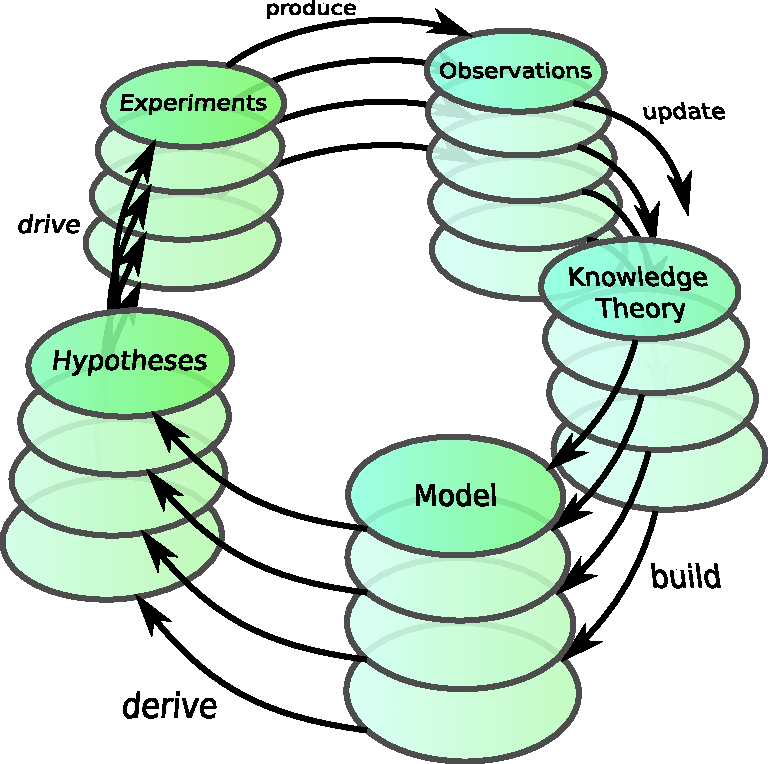
\includegraphics[width=0.35\textwidth]{images/empirical_spiral4}
 \caption{The empirical spiral: applying the empirical cycle in successive
rounds leads to a gradual build-up of knowledge.}\label{fig:empirical-spiral}
\end{figure}


As models are a formalization of knowledge or theories, an underlying formalism is needed to express
this knowledge. Different formal methods have been successfully applied to construct representations
of biological systems. Among these methods are Boolean logic~\citep{boolean-networks-flower,boolean-networks2},
ordinary differential equations (ODEs, reviewed by~\citealp[]{hidde-review}),
interacting state machines~\citep{interacting-sm1,interacting-sm2},
process calculi~\citep{blenx,bio-pepa}, Timed Automata~\citep{ta-siebert,bartocci-oscillators,
oded-ode-ta-discretization} and Petri nets~\citep{petri-nets,petri-nets2}.
Most of these formal methods have been implemented into software tools to aid the process
of modelling. Due to the lack of such a supporting tool, \tas\ have remained a less 
frequently applied method.

\tas\ have been developed to model the dynamic behaviour of systems with processes running in parallel~\citep{timed-automata-alur-dill}. 
As such, \tas\ have been applied in communication protocols and industrial control engineering~\citep{ta-audio-protocol,ta-wap-gateway,ta-ws-bap}. The 
parallels between these application areas and regulatory processes in cells have triggered the step towards 
their use in biology.
\cite{ta-siebert} use \tas\ to extend a classical modelling paradigm
~\citep{thomas-formalism}, allowing to add temporal dynamics to gene network models.
\cite{bartocci-oscillators} describe a model of biological oscillators and test 
synchronization properties in this dynamic system.
A discretization of ODEs to \tas\ is proposed by~\citet{oded-ode-ta-discretization}, applying
a translation between the two formalisms to an example gene regulatory network. Two 
different approaches to transforming
a Petri net model into \tas\ are presented by~\citet{ta-giapponesi},
who also address the important issue of state space explosion in their paper.
Finally, \cite{ta-radiazioni} propose an \emph{ad hoc} \tas\ model of a radiation treatment
system, which is then validated through UPPAAL.\\
Each of these approaches has been successfully validated, demonstrating the potential of \tas\
in biological applications. However, these approaches were all limited to simple
or specific examples and none of these modelling methods
has led to a tool implementation of the proposed method to encourage a broader use
of \tas\ in molecular biology.

Mastery of most existing modelling tools requires training and experience in mathematical modelling. 
In this respect, a lack of tradition in quantitative
reasoning and formal methods within the biological community at large is still a stumbling block for
widespread application of modelling of biological systems. Here, we present an intuitive method for the
construction of formal in silico models of the dynamics of molecular networks, supported by a novel,
user friendly modelling tool, ANIMO (Analysis of Networks with Interactive 
MOdelling,~\citealp[]{animo-bibe}). \tas\ are used as the underlying mathematical formalism.

In the Methods section, we will explain how choosing a suitable abstraction level can make the construction
of models more intuitive. We will then show how ANIMO is designed to support the modelling process following
this approach. Construction of a small model based on experimental data will exemplify the method that we
propose. In the Results section, we first show an ANIMO model of the genes and proteins that constitute
the circadian clock network in \emph{Drosophila Melanogaster}. The remainder of that section is dedicated to
illustrate how a single modelling iteration in the empirical cycle is used to compile prior knowledge and
experimental data into a model, perform \emph{in silico} simulations and derive meaningful testable 
hypotheses. These hypotheses are supported by literature on interactions in different cell types.



\begin{methods}
\section{Methods}
\subsection{Modelling abstractions}\label{subsec:abstractions}

In molecular networks in the cell, cascades of chemical and physical interactions enable propagation of 
signals through the network. In this process, the activity of upstream molecules induces a change in the 
concentration or activity of downstream molecules. For many reactions, the values of the kinetic parameters 
are unknown or difficult to collect. This lack of knowledge hampers the feasibility 
of computational models that describe molecular networks in fine mechanistic detail, especially for larger networks.
As a solution to this problem, we propose the construction of models at a higher level of abstraction, 
thereby reducing the number of parameters involved. In choosing a suitable abstraction level, it is important to 
retain enough descriptive power to give a meaningful formal description of the topology and the 
associated dynamic behavior of biological networks.

As a first abstraction in ANIMO models, the active and inactive forms of each network component 
are represented together by a single node in the network.
Each of these nodes is characterized by its \emph{activity level}, which
represents the fraction of active molecules of that molecular species. When a molecule is known to be 
constitutively active, changes in concentrations of that molecule are treated as changes in its activity level.
Activity levels are discretized into integer variables with a user-defined granularity, ranging from 
Boolean (2 levels) to near-continuous (100 levels).

Detailed biochemical reaction mechanisms are abstracted to \emph{interactions}, which can 
represent either activations ($\rightarrow$) or inhibitions ($\dashv$\,). 
This aggregation of elementary reactions into single interaction steps reduces the number of kinetic 
parameters involved, while preserving cause-and-effect relationships.
For example, consider a reaction in which enzyme $E$ phosphorylates and activates substrate $S$, 
transferring a phosphate group from a molecule of ATP to a molecule of $S$. Biochemically, this reaction 
can be represented as
$$
\mbox{\it E} + \mbox{\it S} + \mbox{\it ATP} \rightleftarrows \mbox{\it ES} + \mbox{\it ATP} \rightarrow \mbox{\it ES}^{\mbox{\scriptsize \it P}} + \mbox{\it ADP} \rightleftarrows \mbox{\it E} + \mbox{\it S}^{\mbox{\scriptsize\it P}} + \mbox{\it ADP},
$$
with conservation condition $\mbox{\it S}_{\mbox{\scriptsize\it tot}} = \mbox{\it S} + \mbox{\it S}^{\mbox{\scriptsize\it P}}$.\\
In an ANIMO model this reaction is abstracted to the corresponding interaction
$$
\mbox{\it E} \rightarrow \mbox{\it S}.
$$
Each occurrence of the interaction $E \rightarrow S$ will increase the activity level of $S$ by one discrete step. 
Since the activity level is defined as the active fraction of a molecular species, an increase in the active fraction
automatically implies a decrease in the inactive fraction. Hence, the original conservation condition is always 
satisfied.
The interaction rate $R$, depends on the activity levels of the reactants involved and on a single kinetic
parameter $k$ that is set by the user. 
The three available interaction scenarios can be interpreted as abstracted kinetic rate laws:
\begin{enumerate}
  \item $R = k \times [E]$: the interaction rate depends only on the activity level of the upstream node.
  \item $R = k \times [E] \times [1 - S]$: the rate depends on the activity levels of both participants. This formula
  gives the rate for an activating interaction, which depends on the presence of inactive substrate, 
  $[1 -S]$. Instead, inhibitionsdepend on the level of active substrate, $[S]$.
  \item $R = k \times [E_1] \times [E_2]$: This scenario can be used when the activition or inhibition
  of a downstream node depends on the simultaneous activity of two upstream nodes. This scenario is comparable to an
  \emph{AND-gate} in Boolean logic.
\end{enumerate}
We will show in Section~\ref{sec:results} that the abstraction proposed here preserves ample
expressivity to capture the dynamic behavior of a biological network. 


\subsection{Modelling interactions with Timed Automata}\label{subsec:timed-automata}
\def\ta{TA}
\def\tas{TA}

The formal model we propose here is based on Timed Automata~(\tas, \citealt{timed-automata-alur-dill}), which is a
formalism developed for modelling dynamic concurrent systems in computer science where timing plays a central role.
Being compositional in nature, \tas\ have been shown to be a suitable solution for
modelling biological processes~\citep{ta-siebert,bartocci-oscillators,oded-ode-ta-discretization}.
Our model is based on the abstraction presented in Sect.~\ref{subsec:abstractions}
and uses the clock mechanism of \tas\ to represent interaction rates:
a faster interaction will take less time than a slower interaction to perform one activation/inhibition step.

Figure~\ref{fig:abstraction-mek-erk} contains a simplified \tas\ model of the activation of extracellular
regulated kinase (ERK) by MAPK ERK kinase (MEK) that illustrates the basic properties of \tas.



\def\mekTA{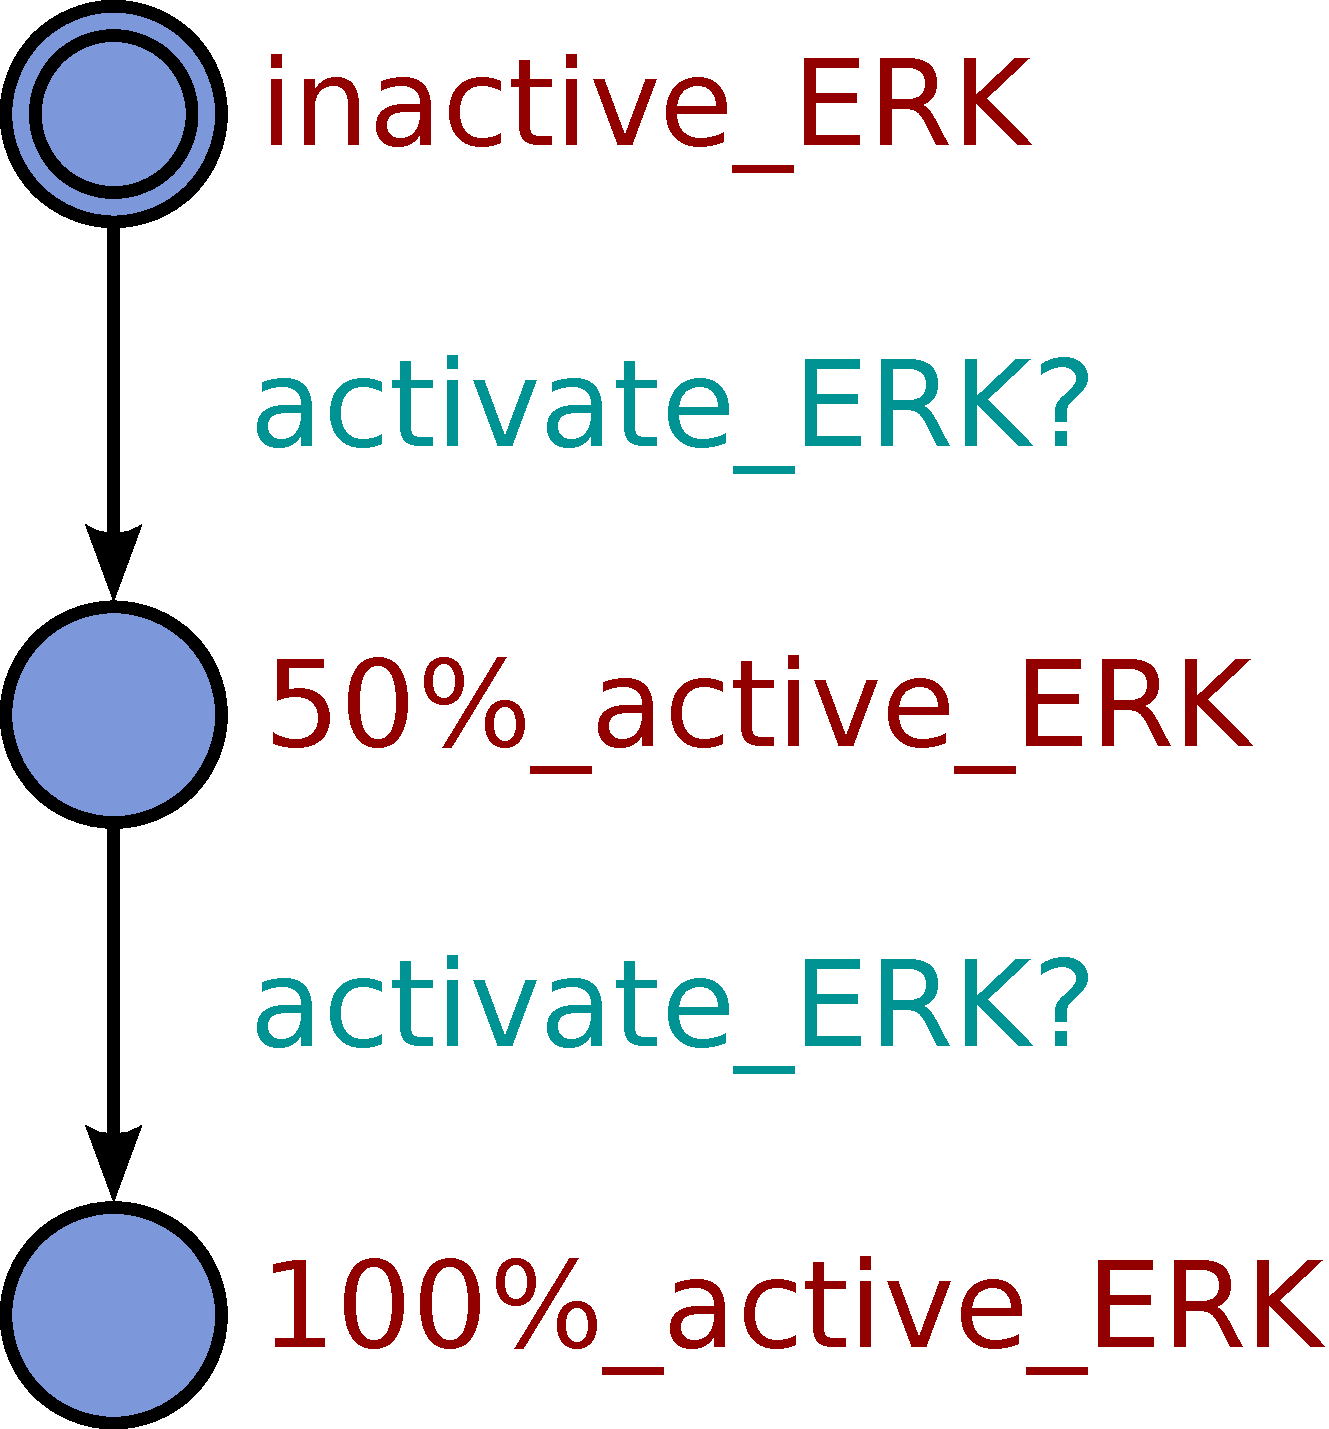
\includegraphics[scale=.098]{images/abstraction_ta_erk3}}
\newlength\mekTAheight
\setlength\mekTAheight{\heightof{\mekTA}}
\begin{figure}[!hb]
%\begin{minipage}{\textwidth}
\begin{center}
\subfloat[\label{subfig:mek-erk}]{\begin{minipage}[c][\mekTAheight]{0.13\textwidth}\begin{center}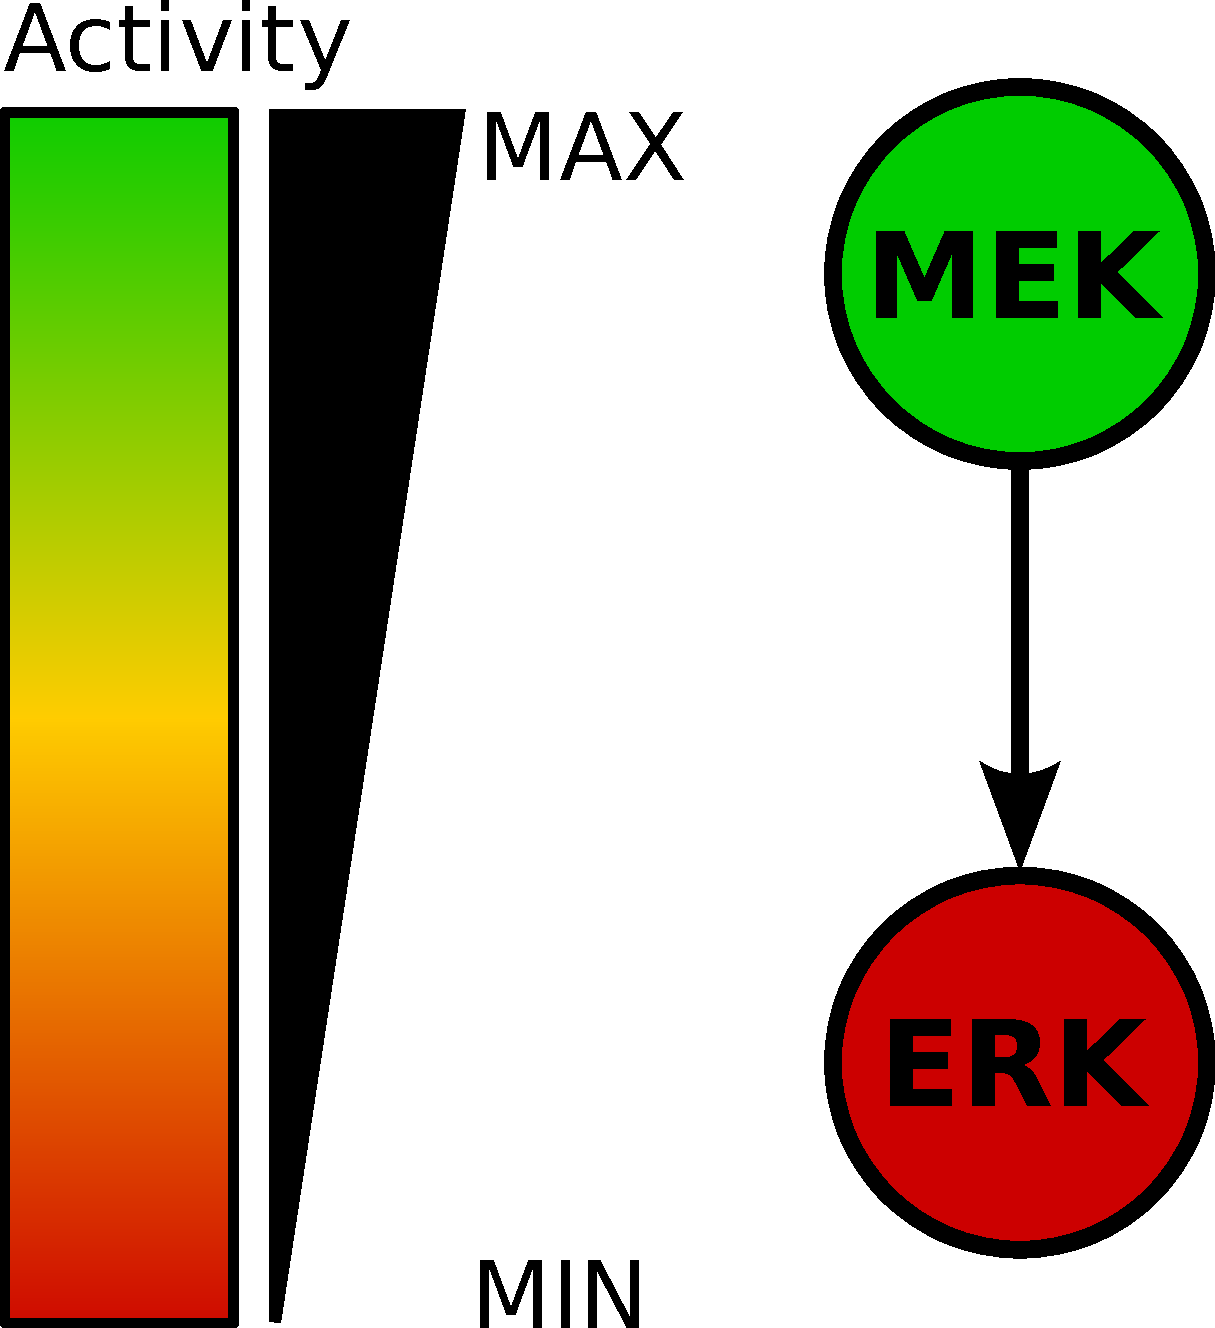
\includegraphics[scale=.098]{images/abstraction_ta_mek-erk3}\end{center}\end{minipage}}
\qquad
\subfloat[\label{subfig:mek}]{\begin{minipage}[c][\mekTAheight]{0.13\textwidth}\begin{center}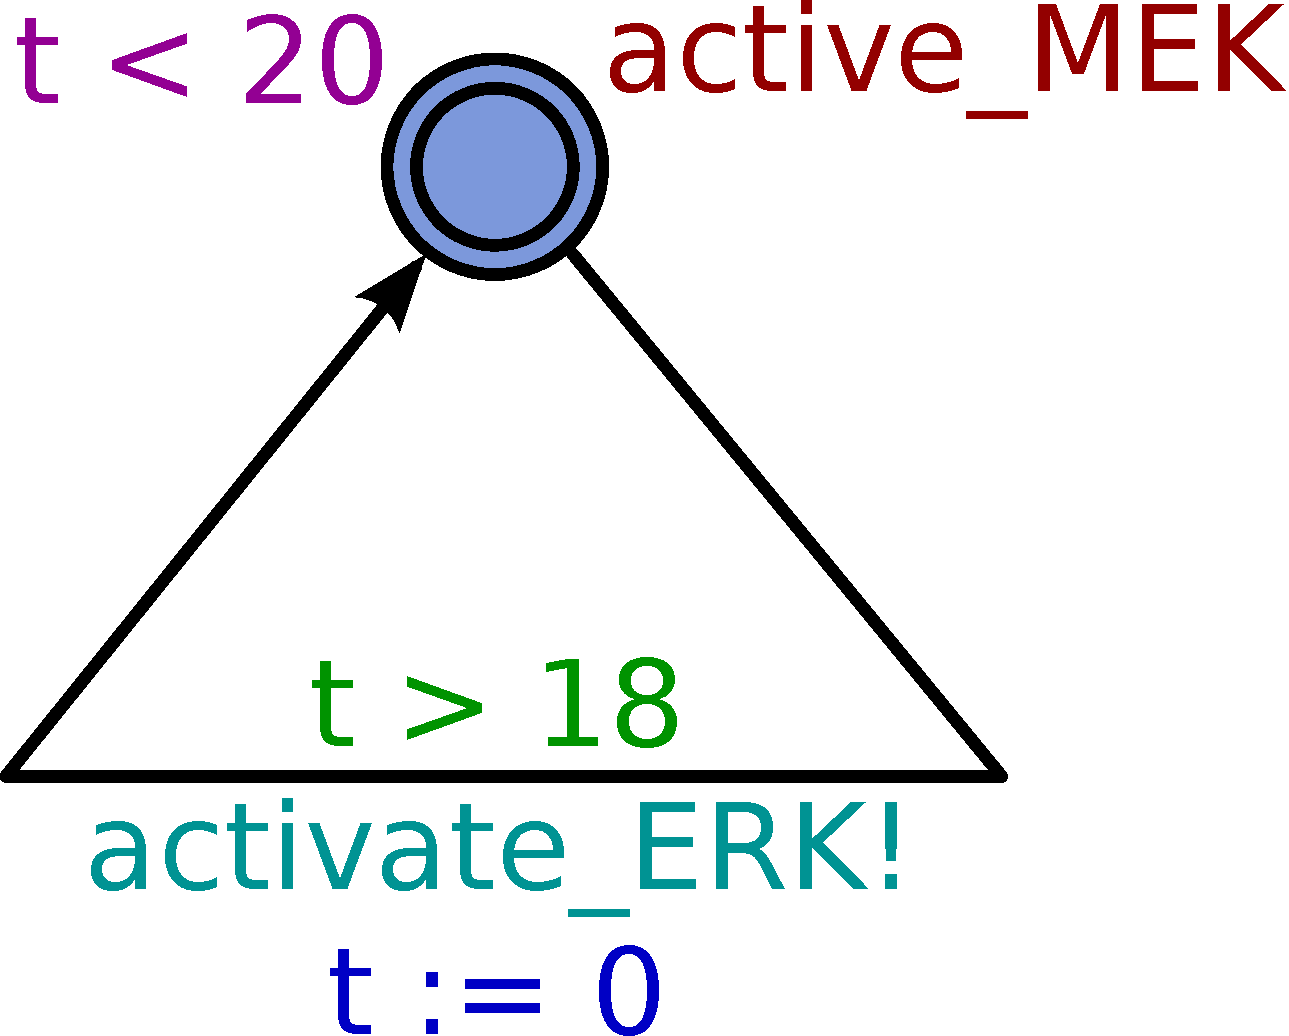
\includegraphics[scale=.098]{images/abstraction_ta_mek}\end{center}\end{minipage}}
\qquad
\subfloat[\label{subfig:erk}]{\begin{minipage}[c][\mekTAheight]{0.14\textwidth}\begin{center}\mekTA\end{center}\end{minipage}}
\end{center}
\caption{Parallel between an abstract activation interaction and its \tas\ model.
{\bf \protect\subref{subfig:mek-erk}}~Classical depiction of a well-studied intracellular signal transduction interaction: protein
MAPK-ERK kinase (MEK, active) activates downstream protein extracellular-regulated kinase (ERK, initially inactive).
In this example, MEK activity is not regulated and ERK has three activity levels,
completely inactive, halfway active and completely active.
{\bf \protect\subref{subfig:mek}}~A \ta\ model of active MEK, consisting of one location (circle) and one
transition (arrow). ${\sf t} < 20$ is termed an invariant on the location, allowing residence in this location as long as local
clock time {\sf t} is smaller than $20$ units. ${\sf t} > 18$ is termed a guard on the transition, allowing the
transition to take place when local clock {\sf t} is greater than $18$ units. Together, the invariant and guard in this
example ensure that the transition must take place within the (continuous) time interval $18 < {\sf t} < 20$. When the
transition takes place, the action {\sf activate\_Erk!} is performed (thus allowing the ERK automaton to reach the {\sf
50\%\_active\_ERK} location) and the local clock coupled to this automaton is reset, ${\sf t} := 0$.
This allows the reaction to occur another time, fully activating ERK.
{\bf \protect\subref{subfig:erk}}~A \ta\ model of ERK, consisting of three locations, {\sf inactive\_ERK}
(the starting location), {\sf 50\%\_active\_ERK} and {\sf 100\%\_active\_ERK},
and two transitions between the locations. A transition will take place when it is possible to synchronize with
the corresponding action {\sf activate\_ERK!} in the MEK automaton.
Each synchronization on channel {\sf activate\_ERK} represents the occurrence of the activating
interaction between MEK and ERK, and allows ERK to eventually become completely active.}\label{fig:abstraction-mek-erk}
%\end{minipage}
\end{figure}





\subsection{ANIMO}
The modelling approach described in Section~\ref{subsec:abstractions} is implemented in the
software tool ANIMO (Analysis of Networks with Interactive MOdelling, \citealt{animo-bibe}),
a plug-in to the network visualization tool Cytoscape~\citep{cytoscape}. The visual interface of ANIMO
is designed to allow the user to intuitively construct activity-based models, making the expansion
and rewiring of a network a fast and user-friendly process (see Suppl. Video 1). An ANIMO model can
be analysed through simulation, with the results automatically plotted as a graph.
The dynamic behaviour of a model can then be interactively explored by
acting on a slider to highlight time points in a simulation. The selected simulation
point defines the appearance of the network: each node will be coloured depending on its activity level
at the selected simulation instant. Moreover, experimental data can be matched against
the predictions of a model, superposing time-based activity series to a graph produced from the model.


Each network built with ANIMO is automatically translated to
a \tas\ model, which is then simulated with the model checking tool UPPAAL~\citep{uppaal},
translating back the results in the proper user-friendly format
(all parts of Figure~\ref{fig:small-model}, as well as similar figures
in the rest of the paper, were taken from ANIMO's user interface).
No training
or prior knowledge on the use of \tas\ or UPPAAL is needed in order to benefit from ANIMO.
Nevertheless, the translation process can be followed in a transparent manner if
desired by the user.

The technical foundations of ANIMO have been described by us elsewhere~\citep{animo-bibe}. 
An abstract overview on the \tas\ model can be found in Supplementary Section~\ref{suppl-sec:animo-ta}.


\subsection{Using ANIMO to build a model based on data}\label{subsec:case-study}
To illustrate the process of model building in ANIMO, we consider now an example based on a literature compendium of
signal transduction events in HT-29 human colon carcinoma cells~\citep{pathway-compendium}. This data set comprises triplicate
measurements of 11 different protein activities or post-translational modification states at 13 time points after
treatment with different combinations of tumour necrosis factor-$\alpha$ (TNF$\alpha$), epidermal growth factor (EGF) and insulin.
The data set contains relative protein levels and activities, and no absolute quantities, which is the typical situation in biochemistry.

As a first step, we normalized measurements for each protein to the
maximum value in the complete experiment, resulting in a nondimensionalized data set that is suitable for use with ANIMO.


In Figure~\ref{fig:small-model}, we show the stepwise construction of a model of a small part of the network that is
able to account for measured variations in activity of inhibitor of nuclear factor kappa-B kinase (IKK), c-Jun N-terminal kinase-1 (JNK1),
mitogen-activated protein kinase-activated protein kinase 2 (MK2), Caspase 8 (Casp8) and Caspase 3 (Casp3) upon stimulation with 100
ng/ml TNF$\alpha$. In this example we aimed for inclusion of a minimum number of nodes in the network, while preserving biological relationships.
Multi-step cascades were aggregated into a single step when possible. Parameters for all reactions were set manually, resulting in a close
match between the model and the patterns observed in the dataset.

A more comprehensive version of this model is presented in Section~\ref{subsec:case-study-larger}.

\def\modelGraphScale{0.2}%0.148}%0.215}
\def\legendGraphScale{0.23}%0.16}
\def\halfGraphScale{0.09}%0.067}%0.1075}
\begin{figure}[!bhtp]
\centering
\begin{tabular}{ll}
\subfloat{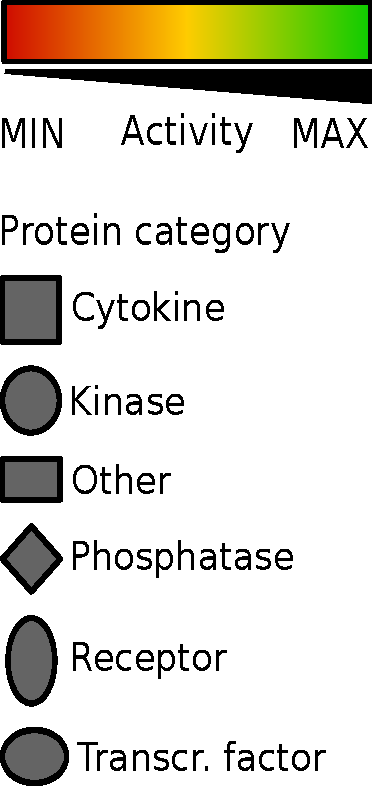
\includegraphics[scale=\legendGraphScale]{images/small-model-1g_legenda}}\addtocounter{subfigure}{-1}\subfloat[\label{fig:small-model-first}]{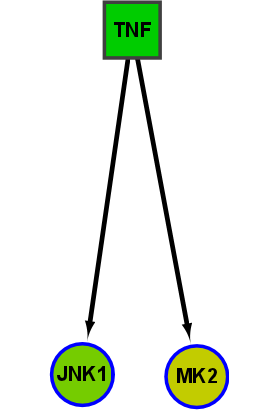
\includegraphics[scale=\modelGraphScale]{images/00-paper-model1f}}
& \subfloat[\label{fig:small-model-first-graph}]{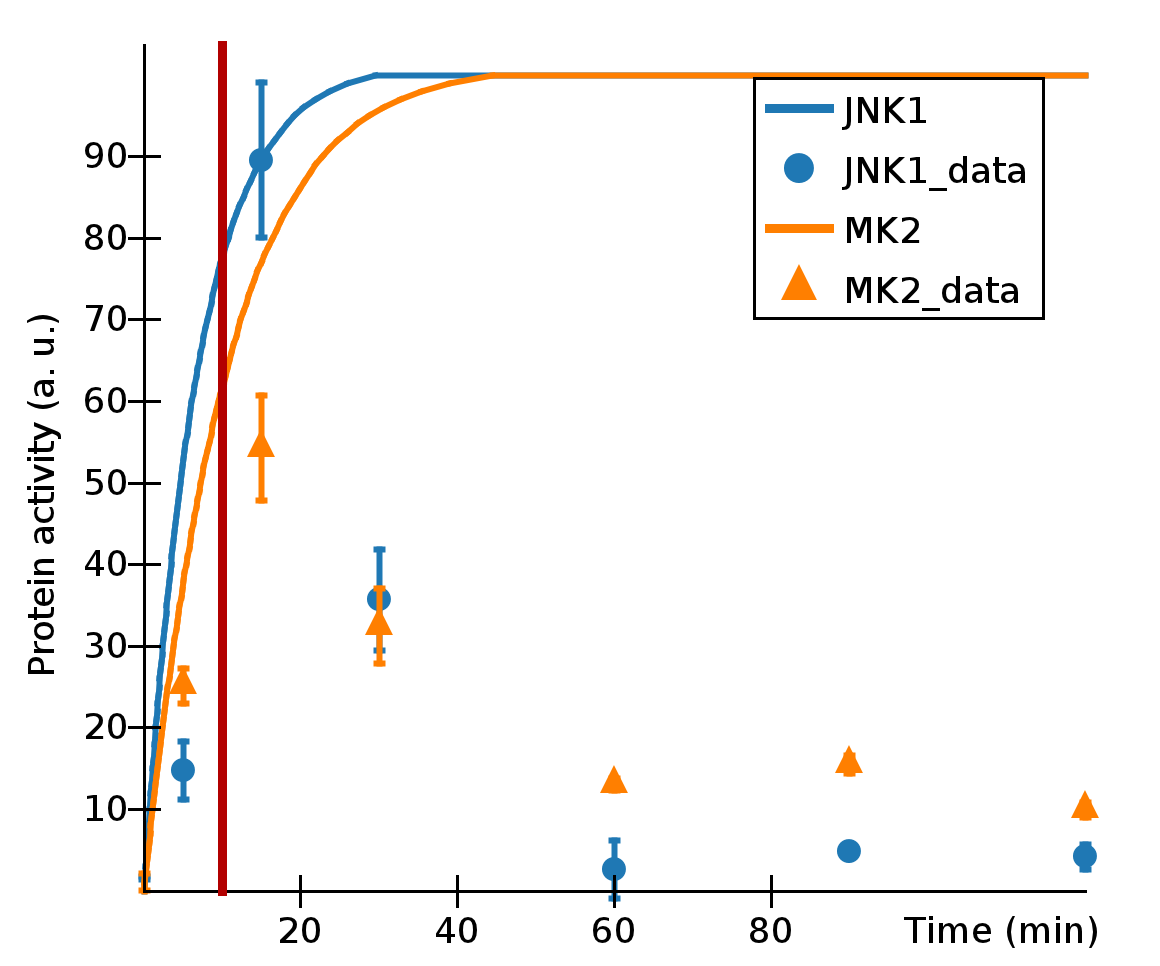
\includegraphics[scale=\halfGraphScale]{images/00-paper-graph1m_riga}} \\[5ex]
\subfloat[\label{fig:small-model-third}]{\qquad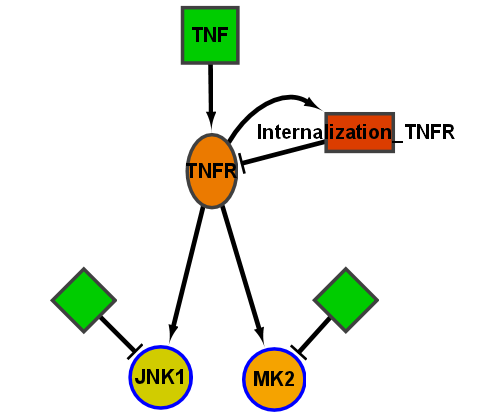
\includegraphics[scale=\modelGraphScale]{images/00-paper-model3f}}
& \subfloat[\label{fig:small-model-third-graph}]{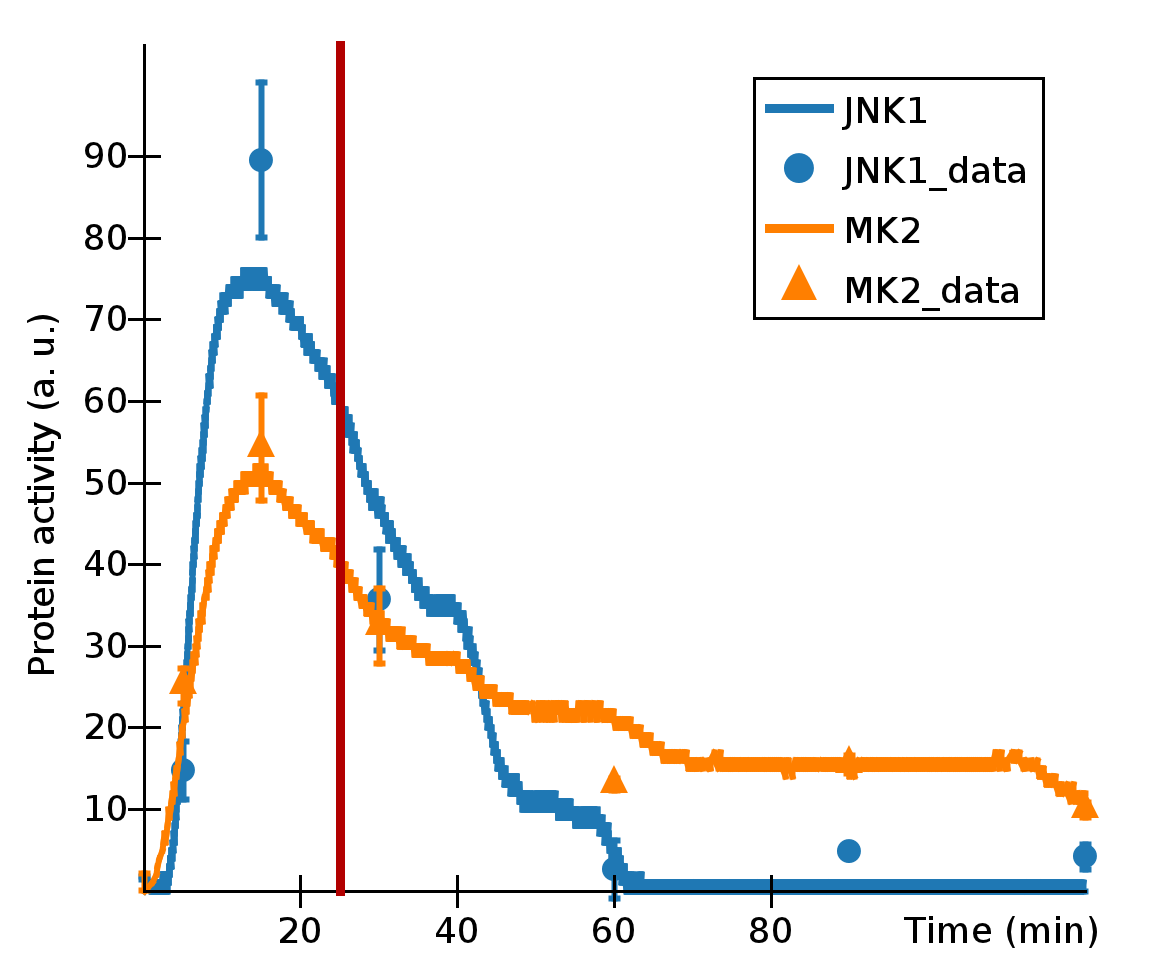
\includegraphics[scale=\halfGraphScale]{images/00-paper-graph3n_riga}} \\[5ex]
\subfloat[\label{fig:small-model-fourth}]{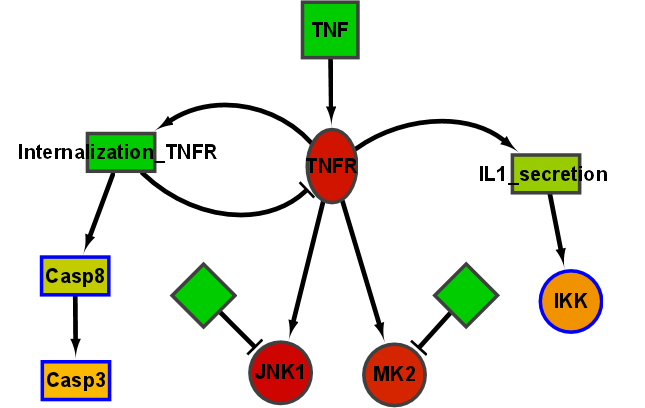
\includegraphics[scale=\modelGraphScale]{images/00-paper-model4g}}
& \subfloat[\label{fig:small-model-fourth-graph}]{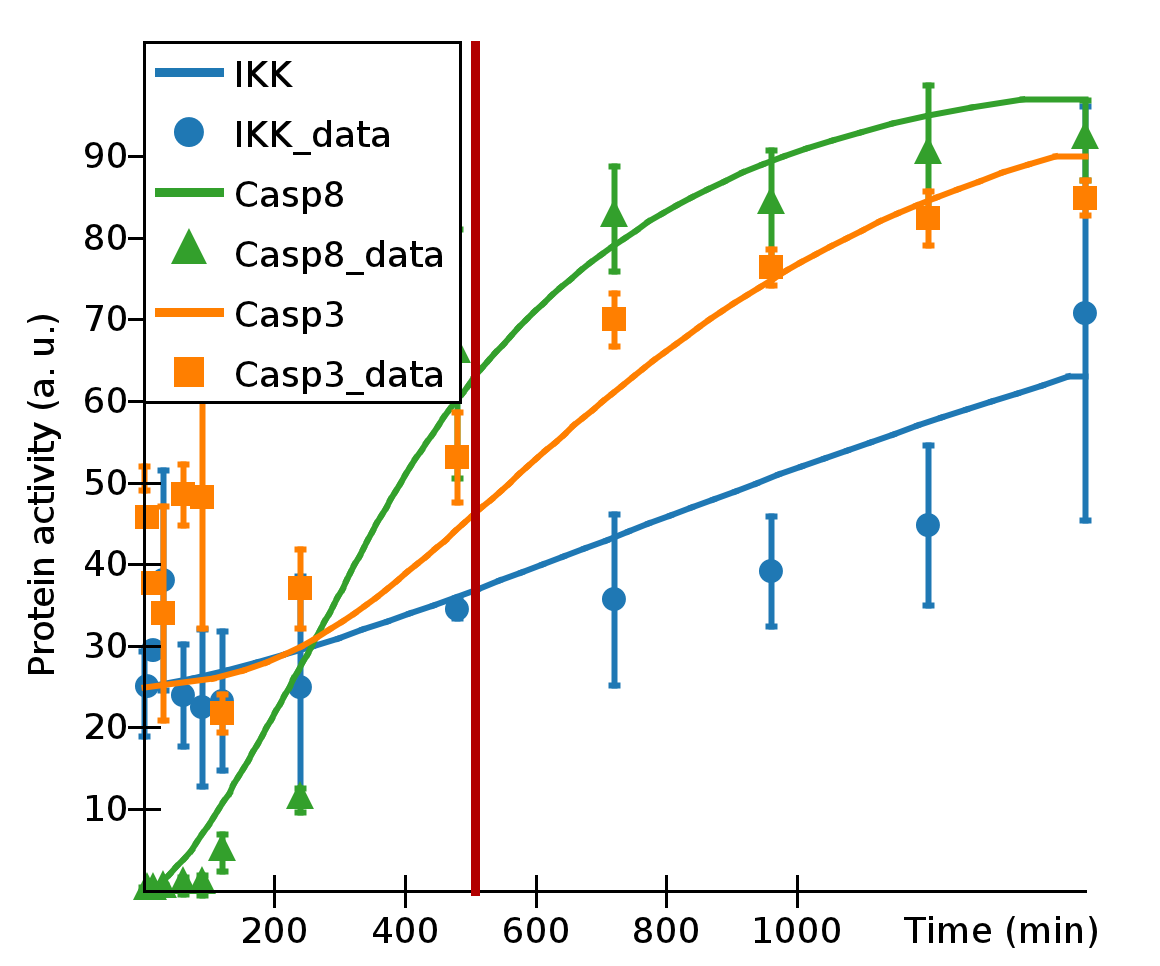
\includegraphics[scale=\halfGraphScale]{images/00-paper-graph4o_riga}}
\end{tabular}
  \caption{
Incremental construction of an ANIMO model of signal transduction
events in human colon carcinoma cells upon stimulation with 100 ng/ml TNF$\alpha$.
Each construction step (top to bottom) is simulated in ANIMO, giving intermediate feedback
useful for the piecewise refinement of the model.
The graphs on the right show the dynamic behaviour of the corresponding models on the left, comparing it to the measured
activity values by~\cite{pathway-compendium} (error bars represent the standard deviation).
On the vertical axis, ``100'' represents the maximum protein activity in the complete experiment.
A red vertical line in each graph highlights a selected time point in the time course:
nodes in the corresponding model are coloured according to their activity at that time point.
{\bf (\protect\subref*{fig:small-model-first}, \protect\subref*{fig:small-model-first-graph})}~Basic model showing direct activation of JNK1 and MK2 by TNF$\alpha$.
No peak dynamics are observed because no inactivating processes are present.
{\bf (\protect\subref*{fig:small-model-third}, \protect\subref*{fig:small-model-third-graph})}~The model after addition of inactivating phosphatases and a
negative feedback loop that down-regulates TNFR (TNF receptor). Note that adding TNFR internalization or phosphatases alone would not be enough to reproduce activity peaks.
{\bf (\protect\subref*{fig:small-model-fourth}, \protect\subref*{fig:small-model-fourth-graph})}~The model after addition of IKK, IL1-secretion (abstracting
the autocrine IL-1 signalling described by~\citealp{pathway-autocrine}), Casp8 and Casp3, showing the late response to TNF$\alpha$ signalling.
As the data set did not contain values for cleaved caspase-3, but only for its non-cleaved precursor pro-caspase-3,
we computed the {\sf Casp3\_{}data} series as $100\% - [\mbox{\sf pro-Casp3}]$.}\label{fig:small-model}
\end{figure}

\end{methods}




\section{Results}\label{sec:results}
\subsection{Expressivity of ANIMO models}\label{sec:animo-drosophila}
While allowing for a low degree of freedom in setting the parameters of models,
ANIMO is still precise enough to describe the behavior of complex networks.
The results obtained with ANIMO are comparable to the ones obtainable with other modeling
approaches, but the modeling process in ANIMO requires considerably less expertise about the formal foundations.
To demonstrate this, Figure~\ref{subfig:drosophila-model}
represents an ANIMO model of the drosophila circadian clock based on the work by~\cite{drosophila-ode-model}, where ordinary
differential equations (ODEs) were used.
The cyclic behavior of the circadian clock is based on the alternating formation and destruction of the CYC/CLK (cycle/clock) protein complex.
This is in turn regulated by a series of proteins which are produced as a consequence of CYC/CLK formation. The CWO (clockwork orange) protein
is central to the network working, as it degrades the mRNA for most of the involved proteins, thus acting as an inhibitor counterbalancing
the action of CYC/CLK.
The positive influence of the light-regulated cryptochrome CRY on the degradation of TIM is a consequence of the passage between light and dark, allowing
the circadian clock to synchronize to a time zone (see Suppl. Sect.~\ref{suppl:repressilator}).


\def\drosophilaGraphScale{0.069}%0.123}

\begin{figure}[!htpb]
\begin{center}
\subfloat[\label{subfig:drosophila-model}]{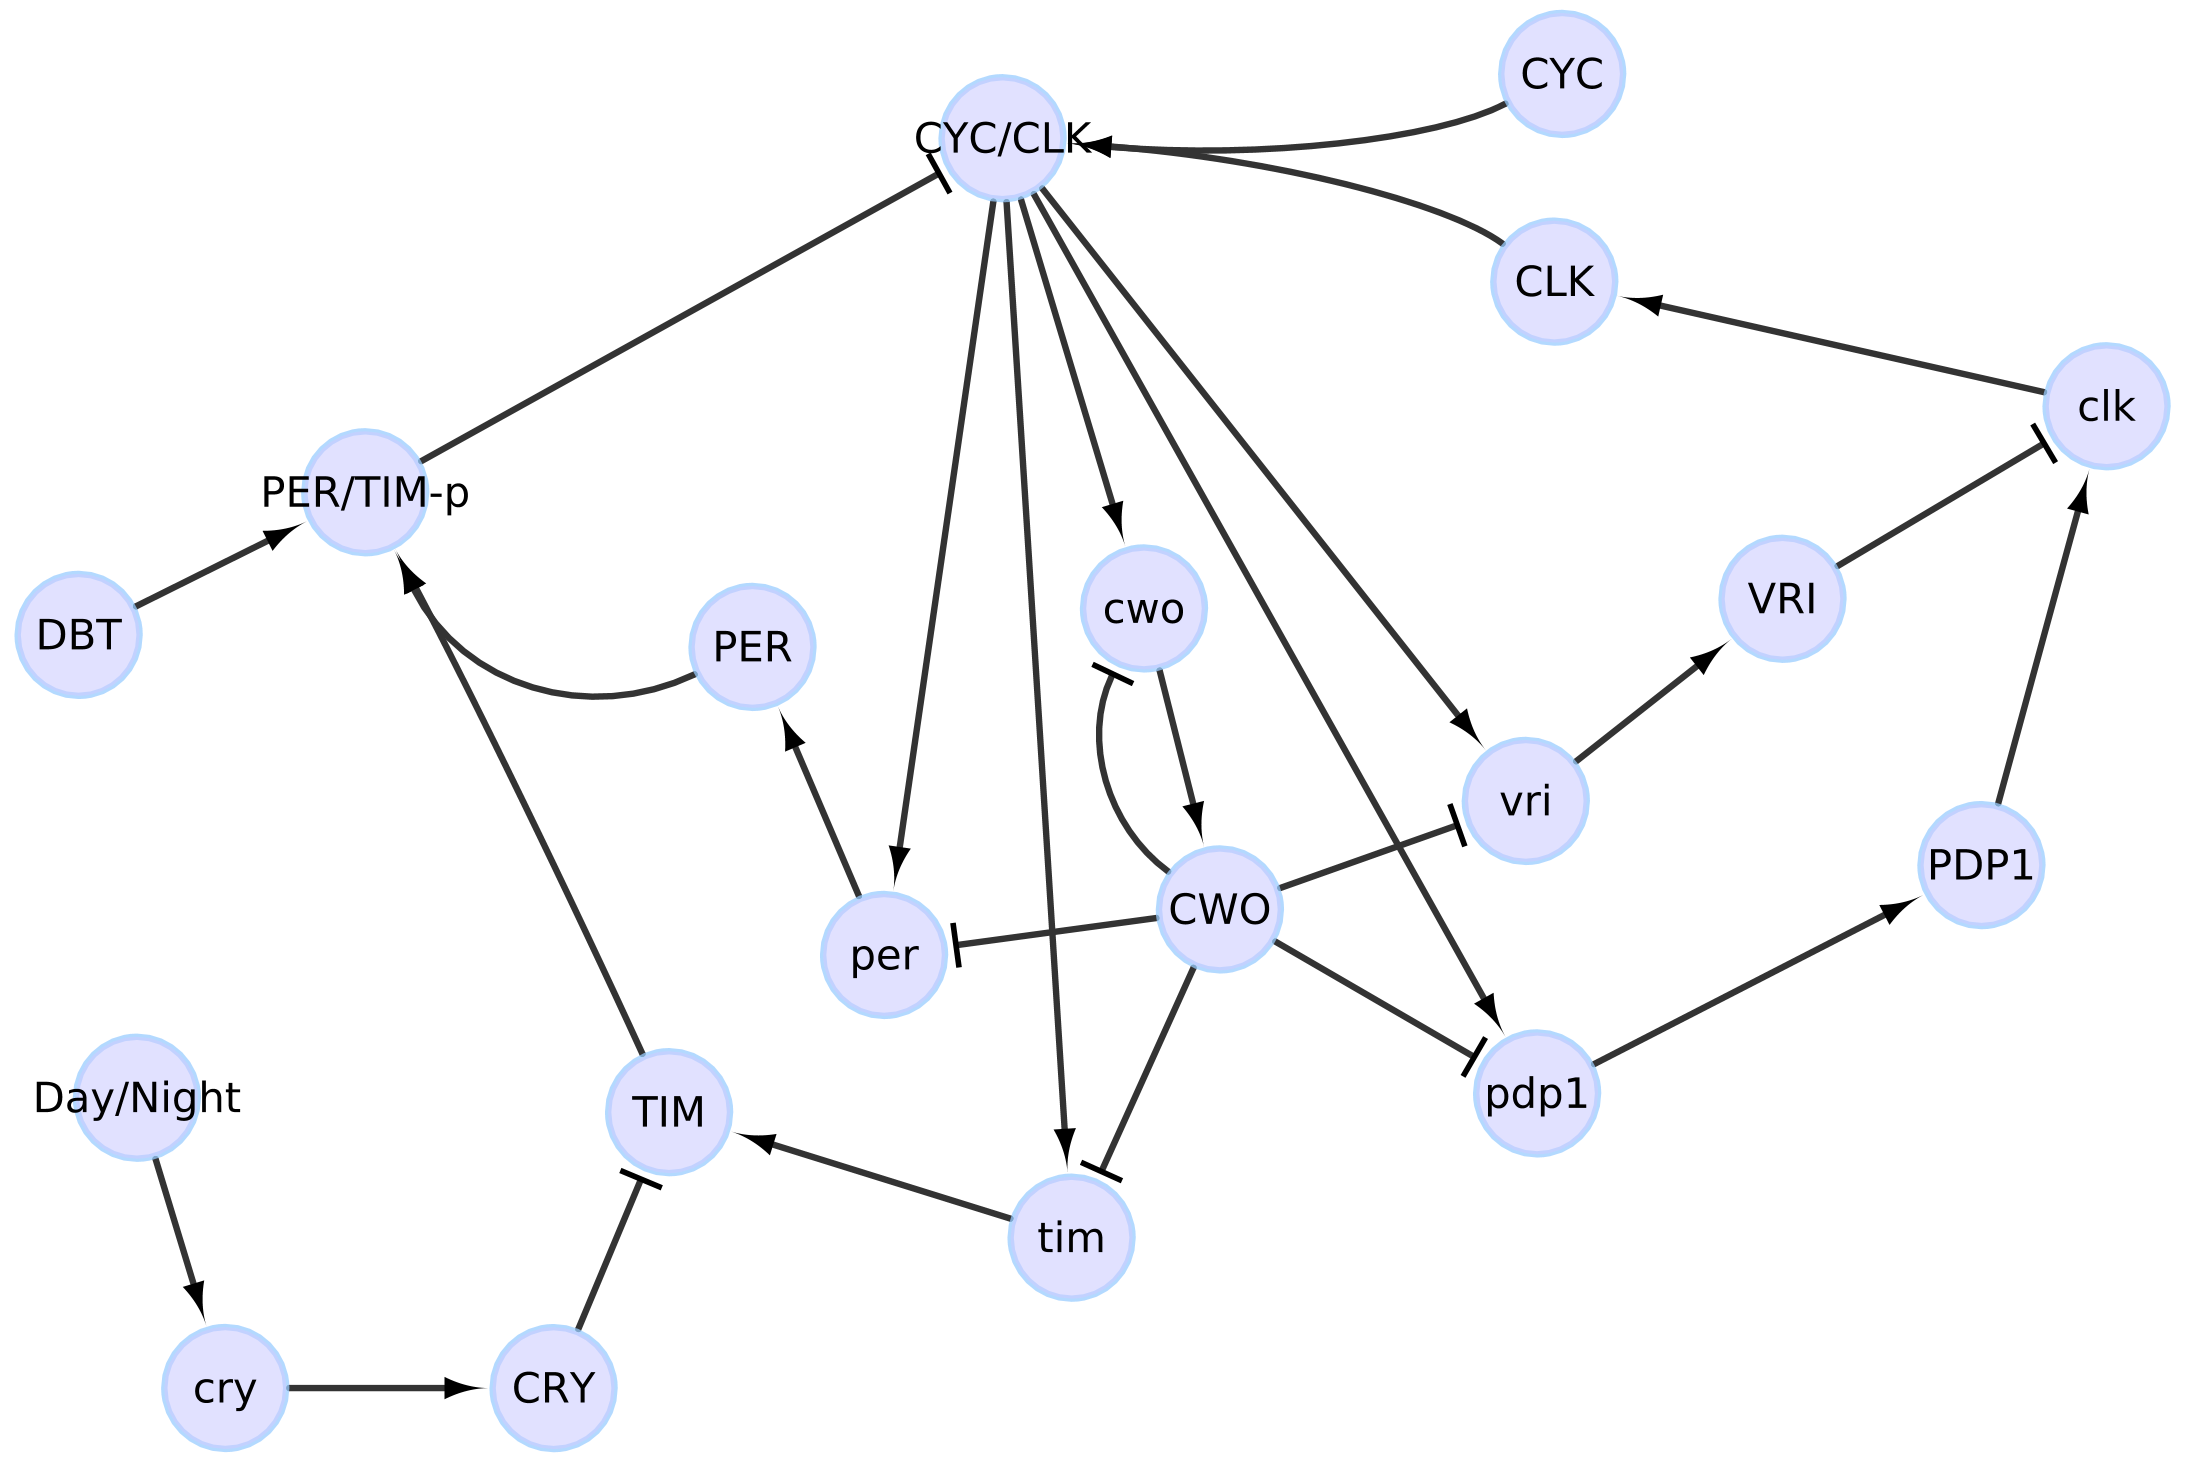
\includegraphics[width=0.49\textwidth]{images/drosophila_model5}}\ %0.85\textwidth
\subfloat[\label{subfig:drosophila-mrna}]{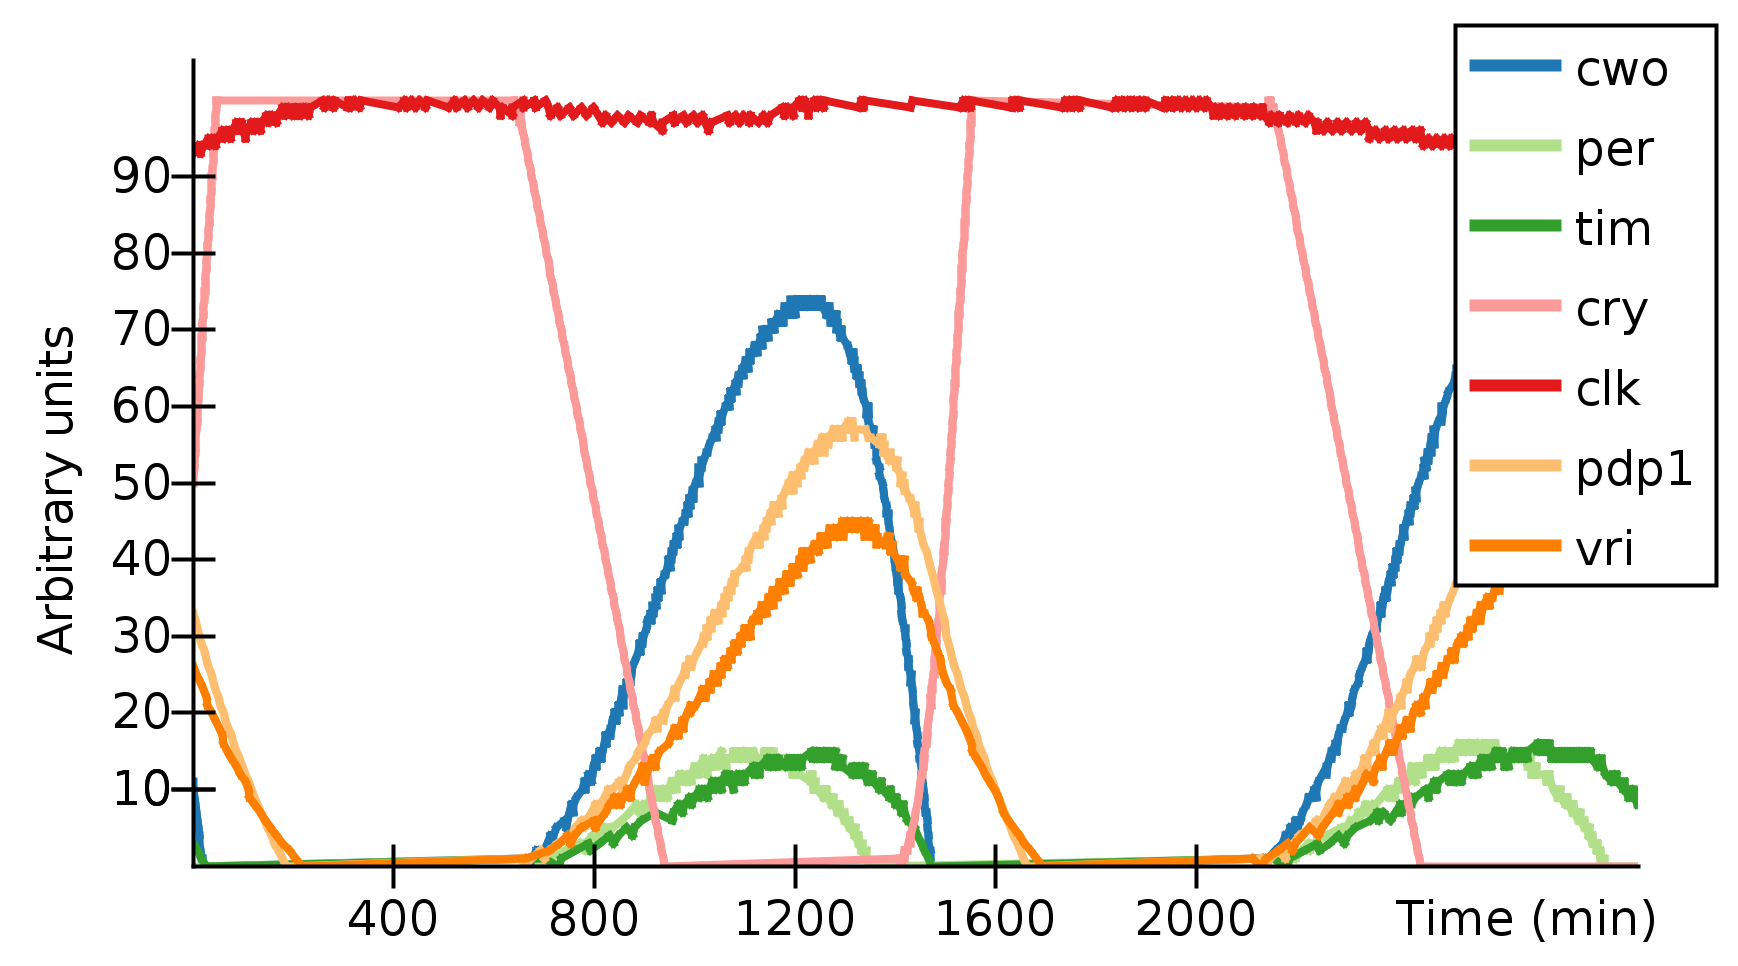
\includegraphics[scale=\drosophilaGraphScale]{images/drosophila_graph2}}\ 
\subfloat[\label{subfig:drosophila-proteins}]{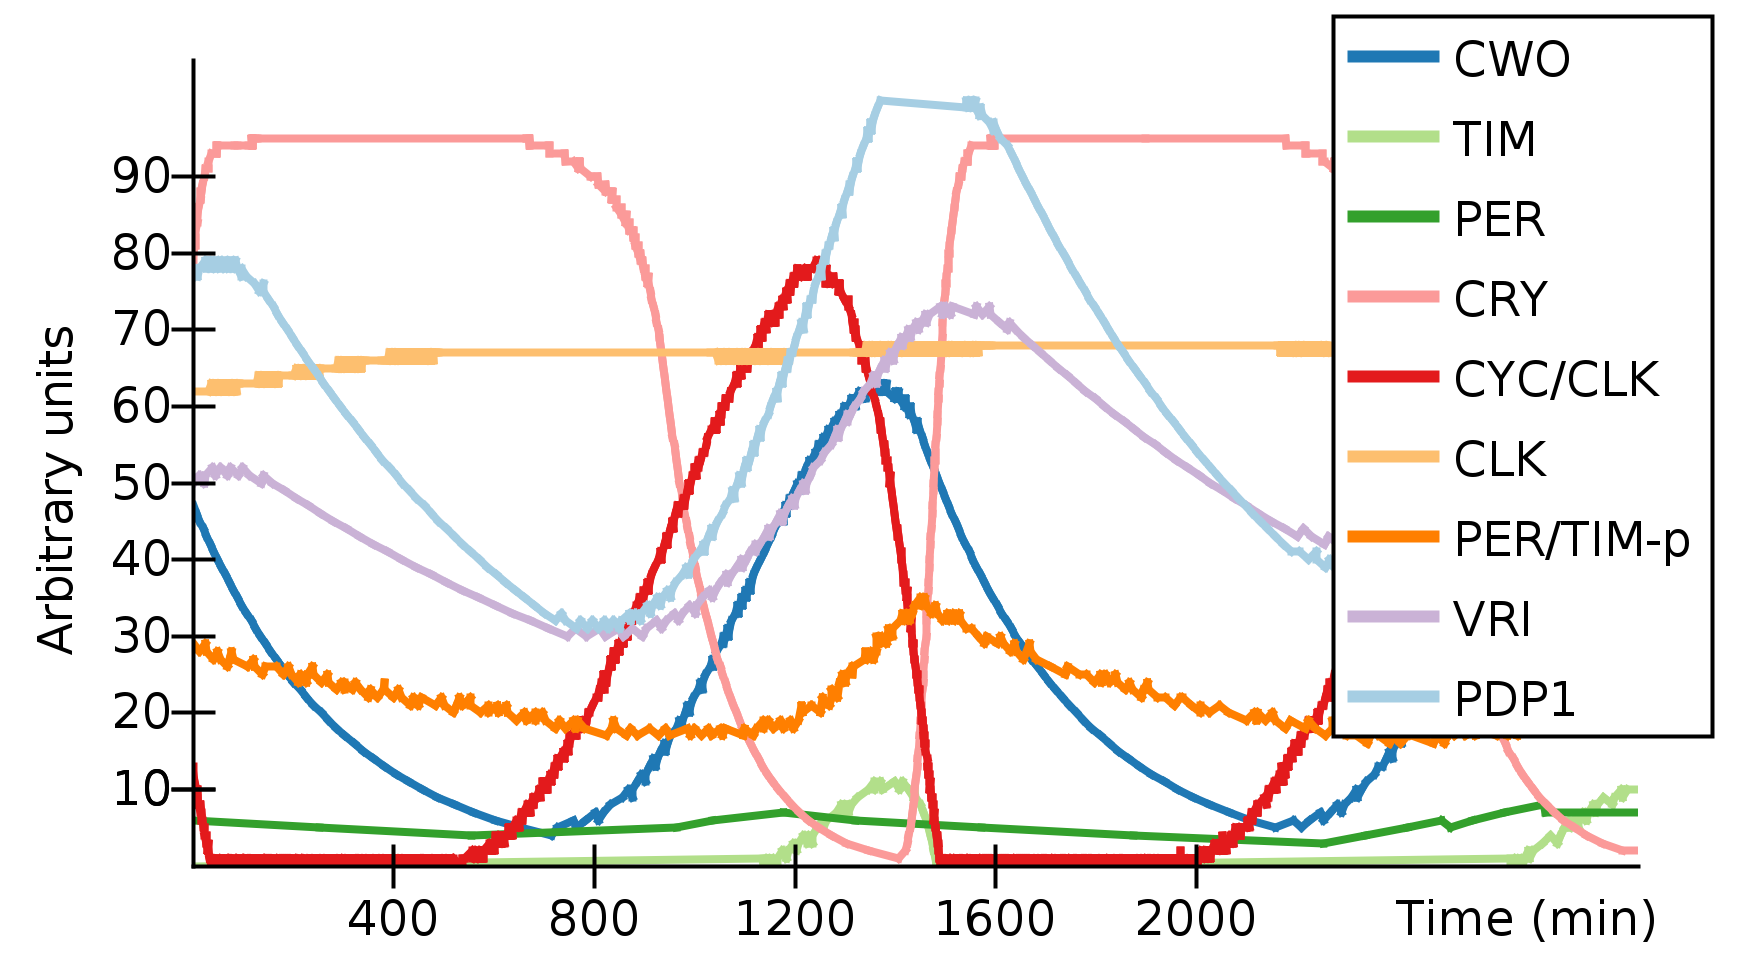
\includegraphics[scale=\drosophilaGraphScale]{images/drosophila_graph1}}
\end{center}
\caption{ANIMO model of the drosophila circadian clock {\bfseries \protect\subref{subfig:drosophila-model}}.
Negative auto-loops on the nodes of the circadian clock network
are also present in the model, following the example of the model by~\cite{drosophila-ode-model}, but are not
represented here only for cosmetic purposes. Naming conventions follow the same rule
as in the original model, with lower-case names representing mRNA, and upper-case names indicating proteins.\\
ANIMO plots of the concentration of
mRNA~{\bfseries \protect\subref{subfig:drosophila-mrna}}
and proteins~{\bfseries \protect\subref{subfig:drosophila-proteins}} over a period of 48~hours.
Oscillations are shown here on an absolute scale, while the graphs in~\citep{drosophila-ode-model}
are based on relative scales, where each series was normalized considering
local minimum and maximum values.}\label{fig:drosophila}
\end{figure}


We see in Figures~\ref{subfig:drosophila-mrna} and~\ref{subfig:drosophila-proteins} that the modeling
power of ANIMO is sufficient to reproduce the cyclic behavior of the model.
In particular, the oscillations exhibited by the two models show the same periods and phases.
Moreover, the ANIMO user interface allows for intuitive \emph{in silico} knock-out experiments,
by manually disabling a node in the model. Such experiments have been done before~\citep{drosophila-ode-model} and
give similar results in our model.
% The model we present here is to be intended only as an example of how a rapidly sketched ANIMO model can help
% in reasoning over existing network models, and not as a complete explanation of the circadian clock network.
% Producing a model that closely fits all experimental conditions for the studied network would be outside the scope of this paper.



\subsection{Case study: using ANIMO to generate hypotheses}\label{subsec:case-study-larger}
In order to validate our modeling approach,
we construct a larger model of the signaling network downstream of TNF$\alpha$ and EGF, and formalize crosstalk between the pathways.
 We first modeled the two pathways in isolation~(Figs.~\ref{fig:large-model-tnf}, \ref{fig:large-model-egf}),
using information on protein interactions from
the KEGG~\citep{kegg} and phosphosite~\citep{phosphosite} databases. These models were fitted to the data
from the works by~\citet{pathway-compendium,pathway-autocrine}.
We then merged the two pathways into a single model and added autocrine crosstalk between the pathways that has been
reported previously~\citep{pathway-autocrine}.
Briefly, stimulation with TNF$\alpha$ leads to a rapid release of TGF$\alpha$ ({\sf TGFa} in the model), which activates the EGF receptor ({\sf EGFR}).
This activation causes secretion of IL-1$\alpha$ ({\sf IL-1a}) at later time points.
The effect of IL-1$\alpha$ is down-regulated by the secretion of IL-1 receptor antagonist ({\sf IL-1ra}) downstream of TNF$\alpha$.
The resulting model (Fig.~\ref{fig:large-model-tnf-egf-merged}) was compared to the experimental data for treatments with 100 ng/ml TNF alone
and 100 ng/ml EGF alone (data not shown)~\citep{pathway-compendium}.

At this point, the behavior of the model deviated from the data for some of the nodes.
This is an interesting situation, as it requires
modifications to the model, that can be interpreted as new hypotheses. Below we give two examples and show how
adaptation of the model can be used to generate novel testable hypotheses.



\def\largeModelScale{0.18}%0.15}%0.155}%0.27}
\def\legendScalaColori{0.21}%0.18}%0.21}
\def\legendScalaForme{0.21}%0.18}%0.21}
\def\scalaGrafici{0.0709}%0.13}
\begin{figure}[!htpb]
\centering
 \subfloat[\label{fig:large-model-hypotheses}]{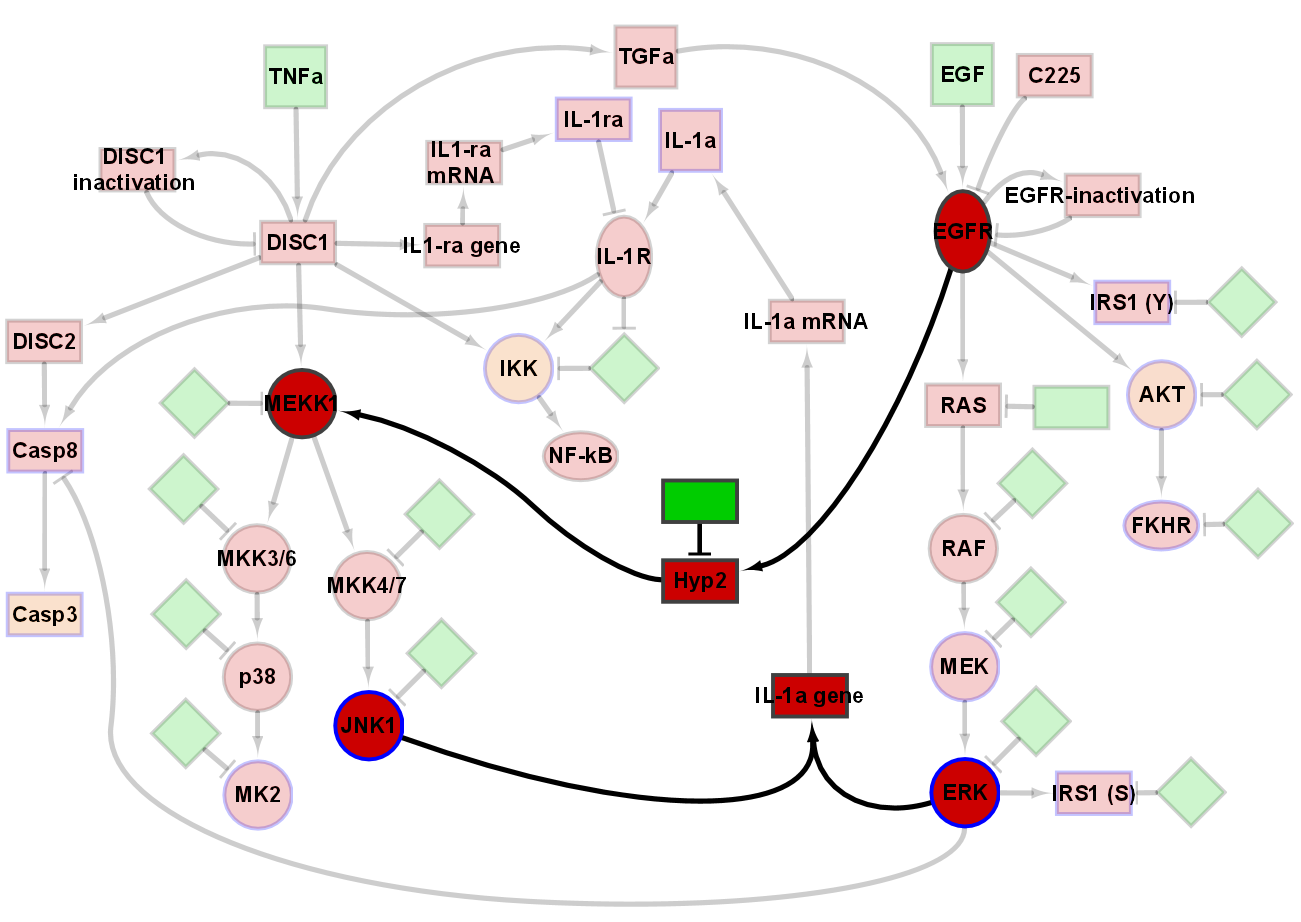
\includegraphics[scale=\largeModelScale]{images/large_network_hypotheses6}}\\
\subfloat[\label{fig:large-model-complete}]{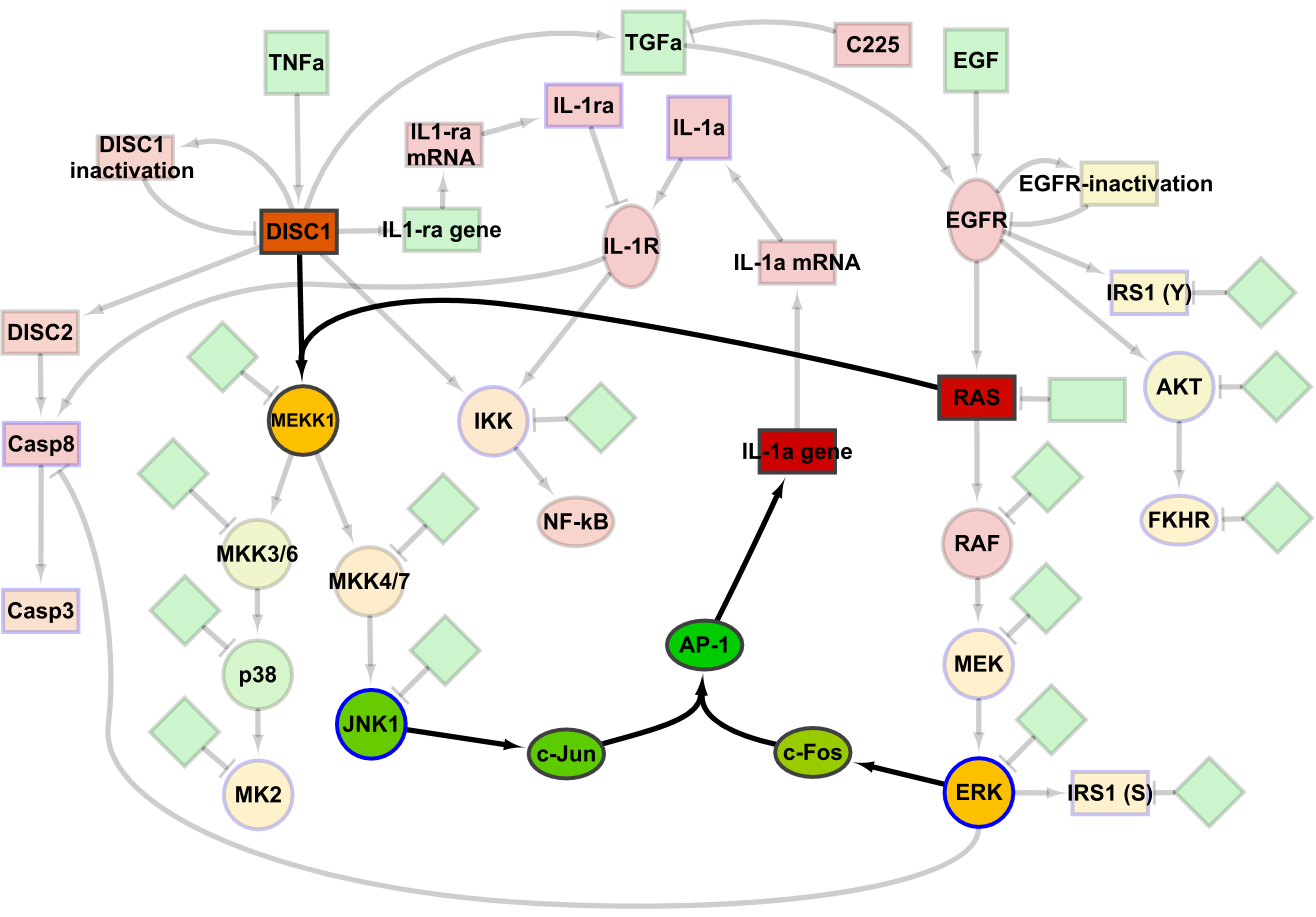
\includegraphics[scale=\largeModelScale]{images/large_network_legendg}}
\\
 \subfloat{
\includegraphics[scale=\legendScalaColori]{images/legenda_forme}}\\ \subfloat{
\includegraphics[scale=\legendScalaForme]{images/legenda_colori}}
\caption{Signaling network downstream of TNF$\alpha$ and EGF in human colon carcinoma cells.
{\bf \protect\subref{fig:large-model-hypotheses}} The merged model for the TNF$\alpha$-EGF pathway in which the two hypotheses are highlighted. Node colors represent initial activity levels.
{\bf \protect\subref{fig:large-model-complete}} The TNF$\alpha$-EGF model with the modified hypotheses. Node colors represent the activity levels $15$ minutes
after stimulation of 100 ng/ml TNF$\alpha$ + 100 ng/ml EGF.}\label{fig:large-model-all}
\end{figure}


Experimentally,
treatment with only TGF$\alpha$ does not lead to secretion of IL-1$\alpha$, for which
 TNF$\alpha$ is also required~\citep{pathway-autocrine}.
However, in the first version of the model TGF$\alpha$ treatment was sufficient for
 IL-1$\alpha$ expression (Fig.~\ref{fig:large-model-graph1}). Given the time delay until secretion of IL-1$\alpha$, it can be
 expected that \emph{de novo} synthesis of IL-1$\alpha$ is required and that both
 TNF$\alpha$ and TGF$\alpha$ are needed to activate transcription of the IL-1$\alpha$ gene.
 JNK1 and ERK signal downstream of TNF$\alpha$ and TGF$\alpha$, respectively, and are known
to affect the activity of many transcription factors. We altered the model to make
 activation of IL-1$\alpha$ expression dependent on both JNK1 activity and ERK activity
(Fig.~\ref{fig:large-model-hypotheses}, arrows linking {\sf JNK1} and {\sf ERK} to {\sf IL-1a gene}).
 After this modification to the model, IL-1$\alpha$ was no longer secreted
upon stimulation with TGF$\alpha$ alone, which greatly improved the fit between the measured IL-1$\alpha$ levels and the model (see
 Fig.~\ref{fig:large-model-graph2}). This hypothesis of IL-1$\alpha$ as a target of combined JNK1 activity and
 ERK activity is supported in literature. Transcription factors c-Jun and c-Fos together
 form a heterodimer known as AP-1 and are activated by JNK1 and ERK,
respectively~\citep{jnk-signaling,cfos-cjun}. AP-1 has been reported to bind to the
 promoter of IL-1$\alpha$, supporting its role in the regulation of IL-1$\alpha$
 expression~\citep{ap1-il1a}. Based on these findings in literature we included c-Jun and
c-Fos in our model as transcriptional activators of IL-1$\alpha$ (Fig.\ref{fig:large-model-complete}).


\begin{figure}[!tpb]
\begin{center}
 \subfloat[\label{fig:large-model-graph1}]{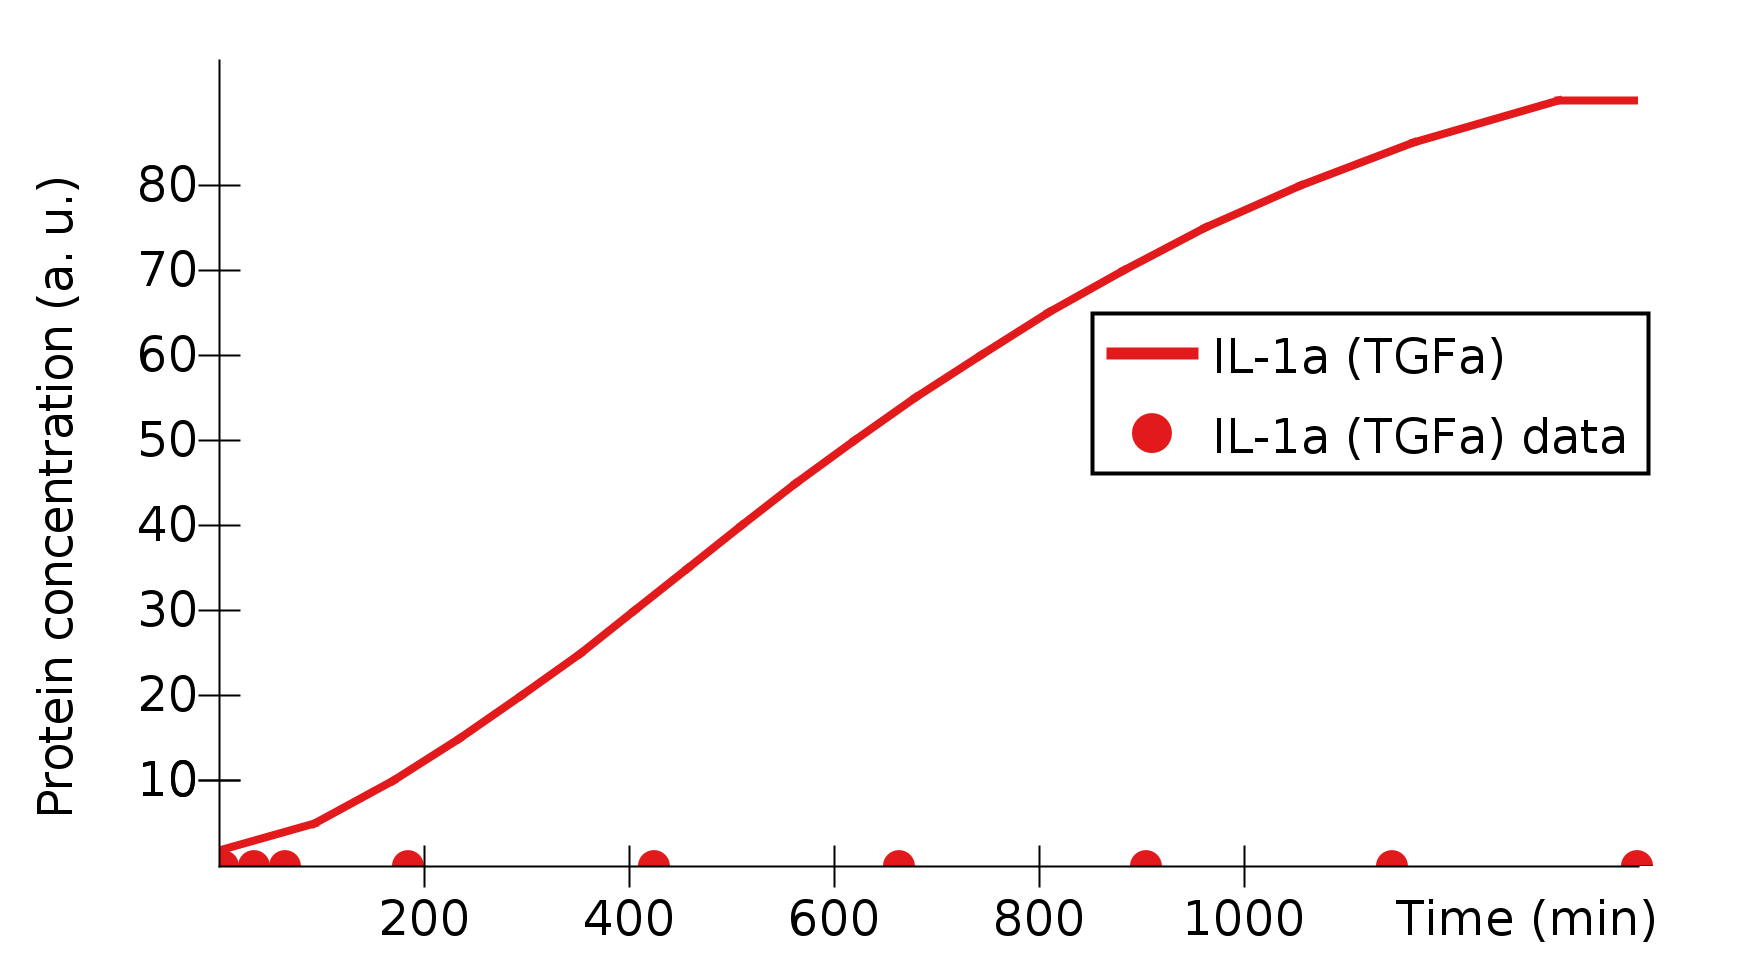
\includegraphics[scale=\scalaGrafici]{images/TGF100_TNF0_ho_hyp_IL-1a3}}
 \subfloat[\label{fig:large-model-graph2}]{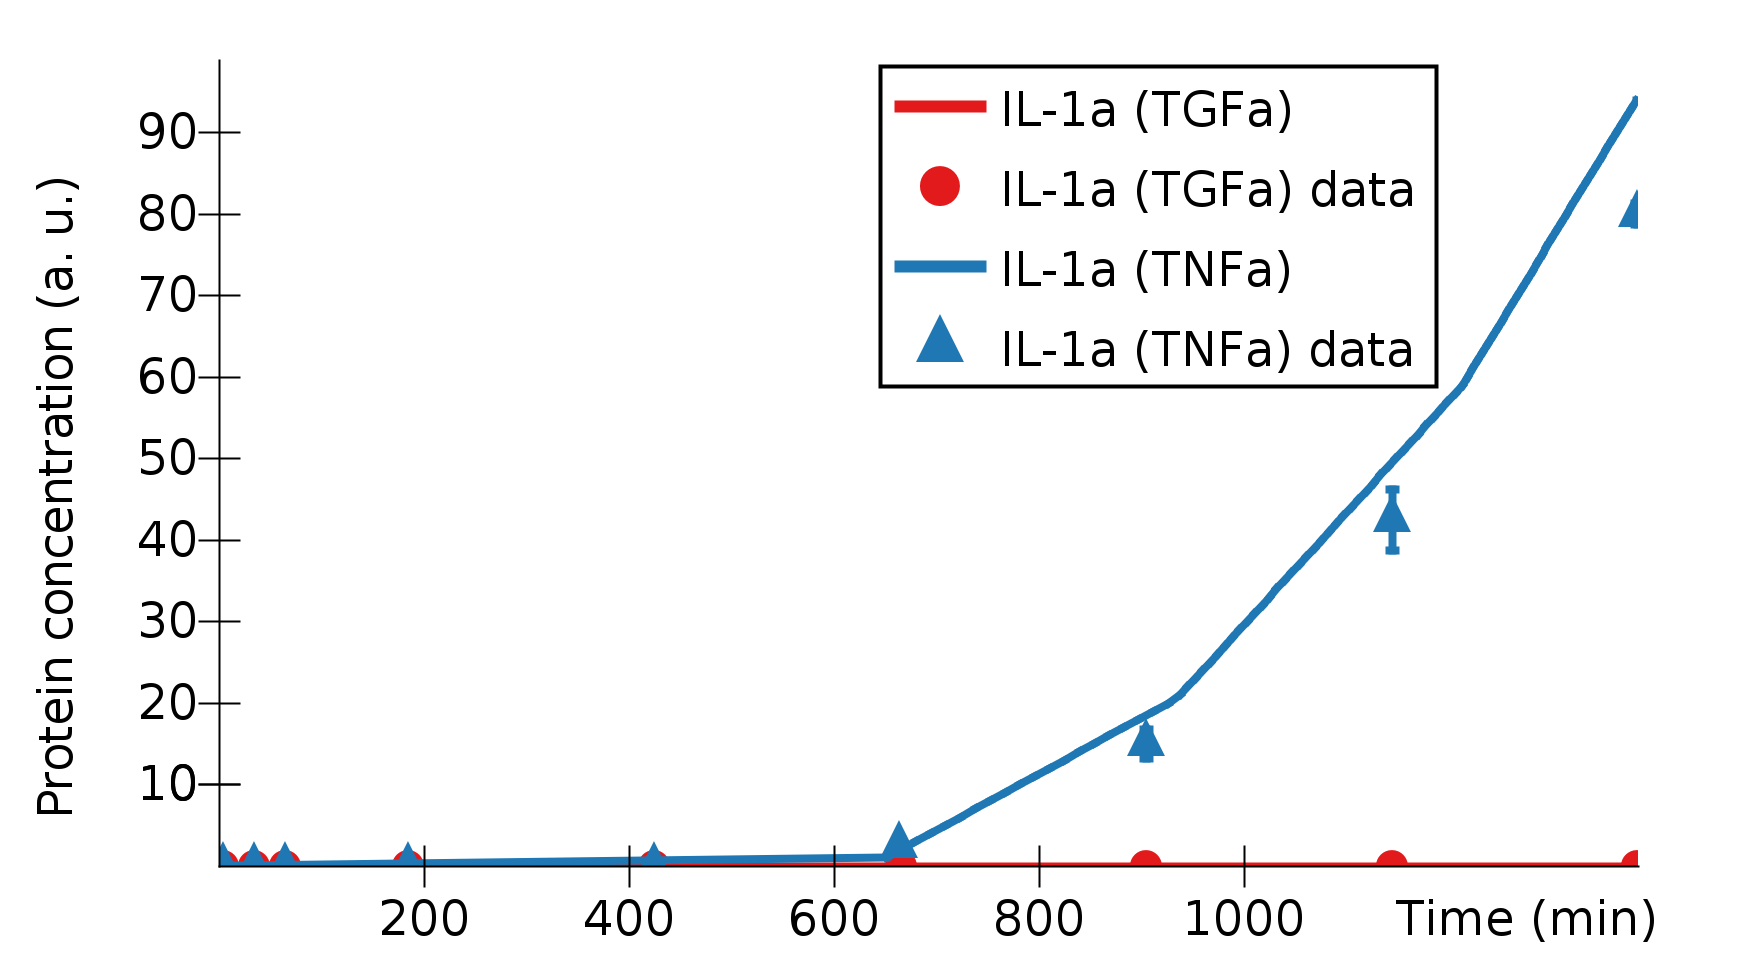
\includegraphics[scale=\scalaGrafici]{images/TGF100_vs_TNF100_hyp1_IL-1a4}}\\
 \subfloat[\label{fig:large-model-graph3}]{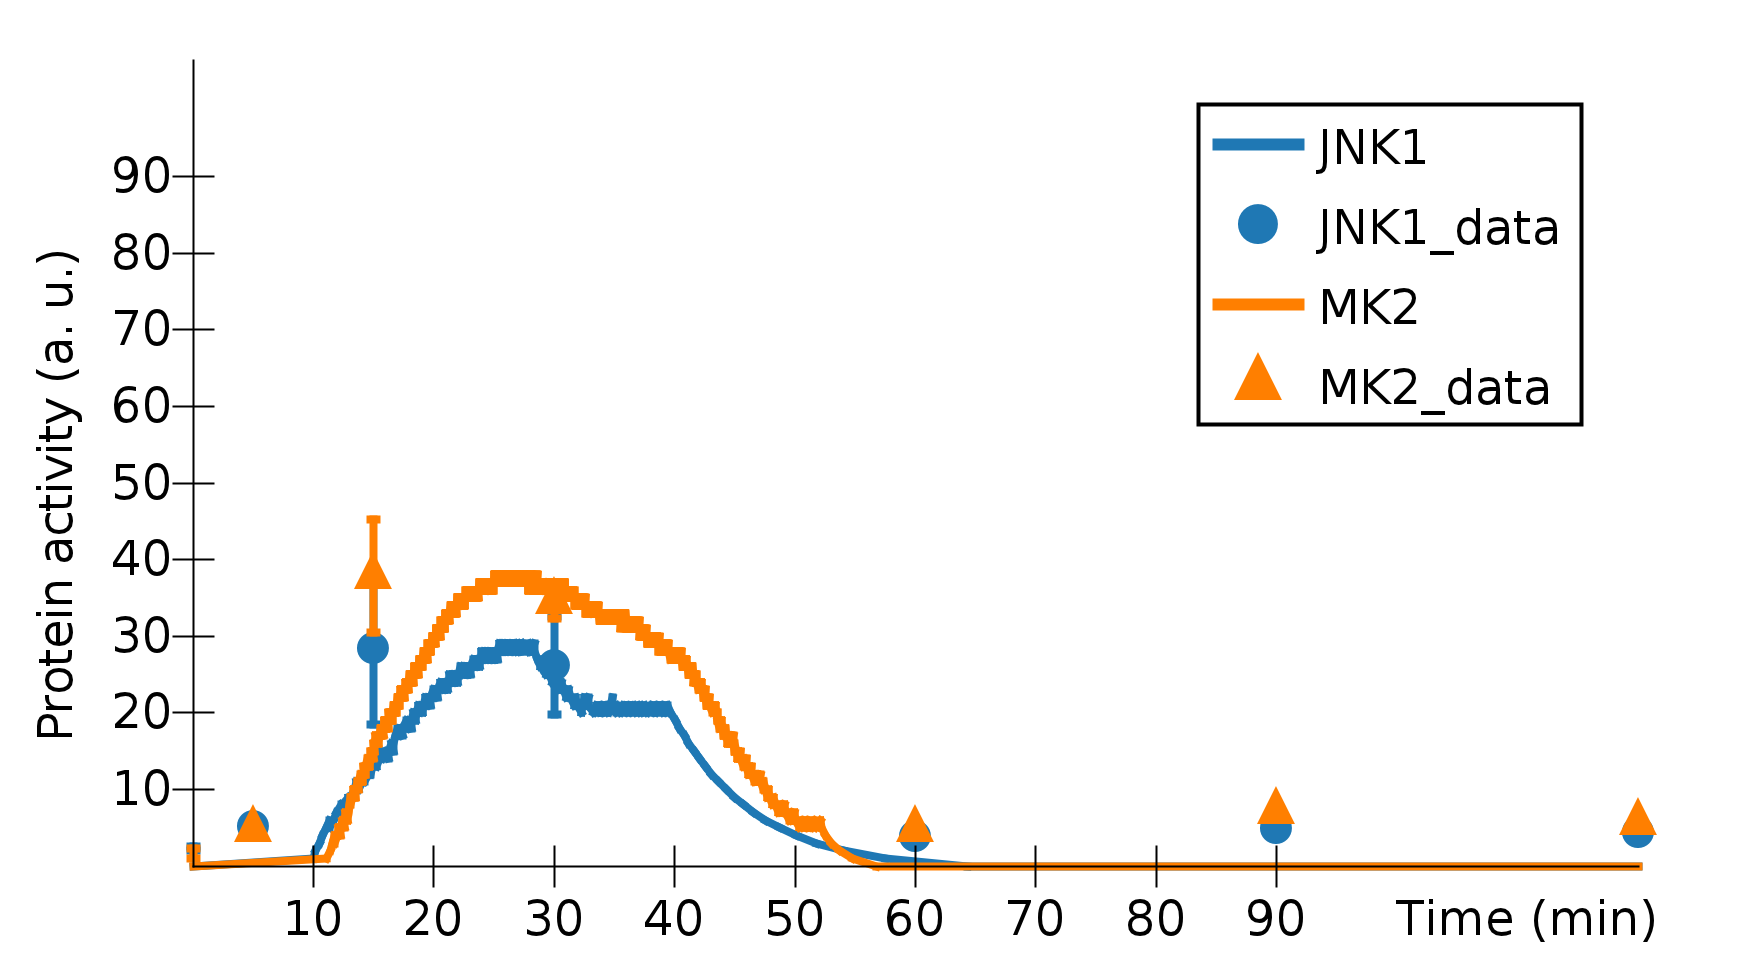
\includegraphics[scale=\scalaGrafici]{images/TNF5_hyp2_JNk1_MK2_3}}
 \subfloat[\label{fig:large-model-graph4}]{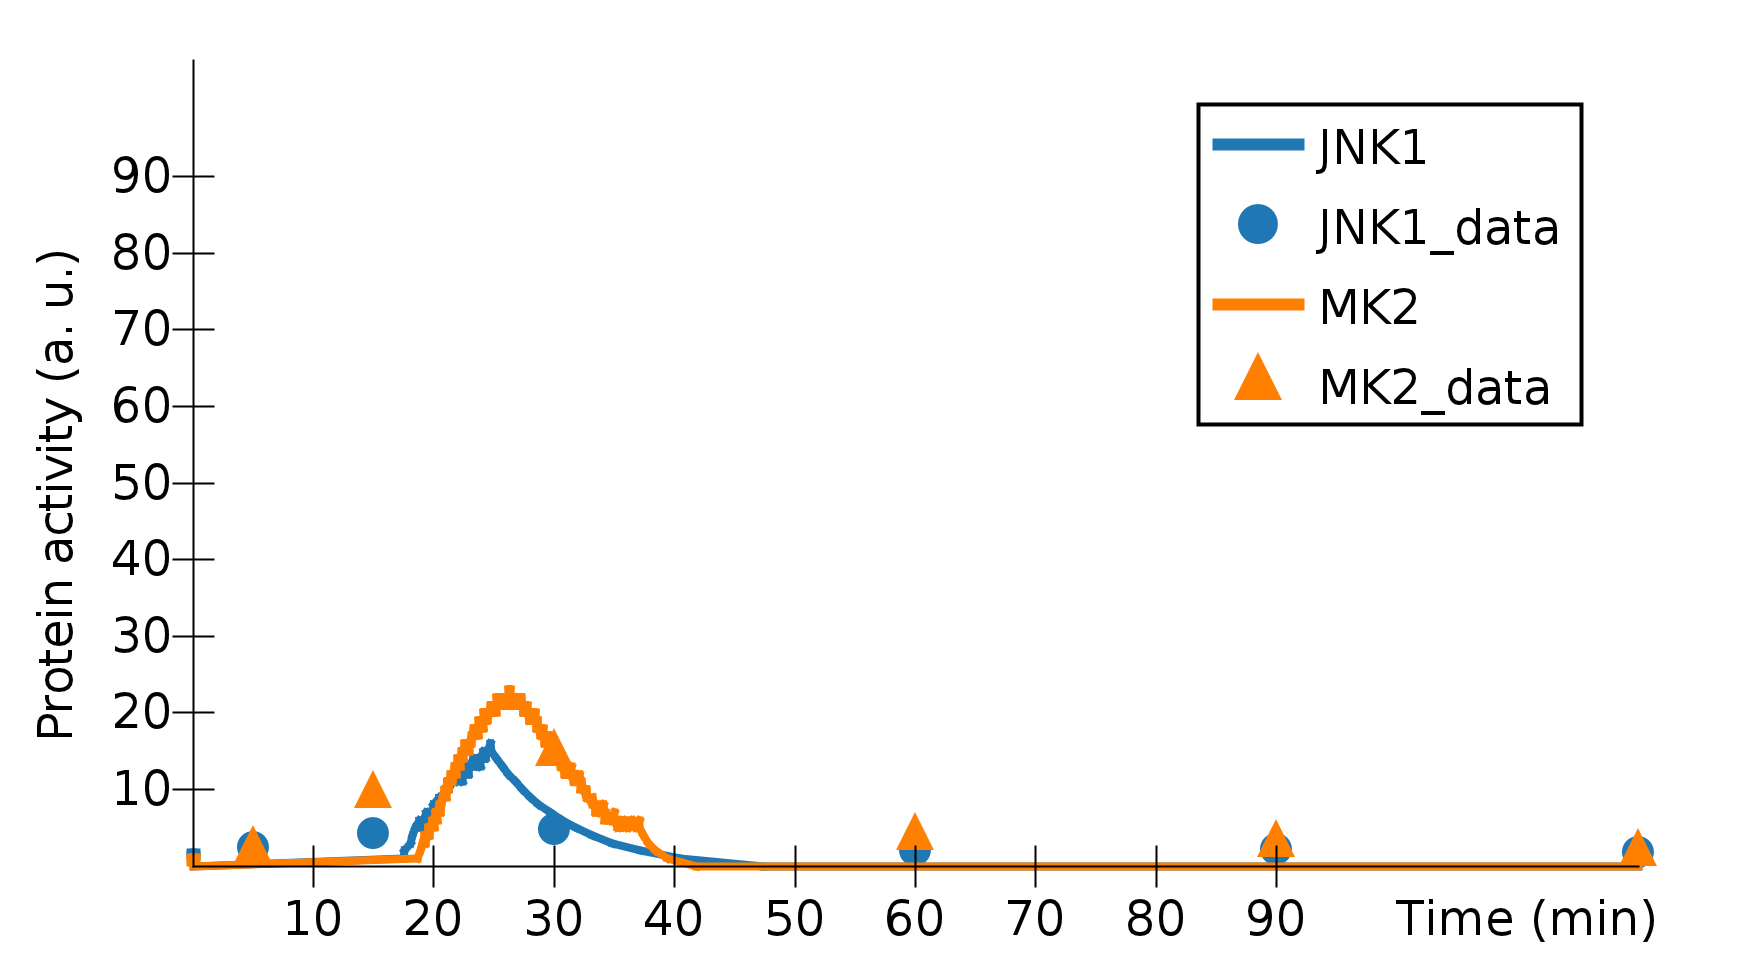
\includegraphics[scale=\scalaGrafici]{images/TNF5_C225_hyp2_JNk1_MK2_3}}
\end{center}
\caption{\scriptsize
Comparison of simulation data obtained from the ANIMO model with experimental data.
{\bf \protect\subref{fig:large-model-graph1}}~Modeled production of IL-1$\alpha$ after stimulation with 100 ng/ml TGF$\alpha$ (24 hours).
{\bf \protect\subref{fig:large-model-graph2}}~After the addition of the first hypothesis (activation of IL-1$\alpha$ production depending both
on JNK1 and ERK): production of IL-1$\alpha$ after stimulation with 100 ng/ml TNF$\alpha$ (series {\sf IL-1a~(TNFa)})
compared with stimulation with 100 ng/ml TGF$\alpha$ (series {\sf IL-1a~(TGFa)}) (24 hours).\\
After the addition of the second hypothesis (activation of MEKK1 downstream of EGFR): {\bf \protect\subref{fig:large-model-graph3}}~stimulation with 5 ng/ml TNF$\alpha$ (2 hours),
{\bf \protect\subref{fig:large-model-graph4}}~stimulation with 5 ng/ml TNF$\alpha$ + 10 $\mu$g/ml C225 (2 hours).
Suppl. Sect.~\ref{suppl:parameters-tnf-egf} explains how the dosage of 5 ng/ml TNF$\alpha$ was represented in the model.}\label{fig:large-model-graph}
\end{figure}


As a second example we considered the behavior of JNK1 and MK2. In the model, both
 proteins were located downstream of TNF$\alpha$ but not TGF$\alpha$ or EGF. Hence, the
 model did not show an effect of C225, a pharmacological inhibitor of ligand-EGFR
 binding, on activation of JNK1 or MK2 after stimulation with TNF$\alpha$. However, experimental
data show that C225 strongly reduces activation of JNK1 and MK2 upon stimulation with TNF$\alpha$~\citep{pathway-autocrine}.
This fact is indicative of a role for EGFR in activation of JNK1 and MK2. Since both JNK1 and MK2
 are located downstream of MAPK/ERK kinase kinase 1 (MEKK1), we hypothesized that activation
 of MEKK1 is dependent on
 both TNF$\alpha$-signaling and TGF$\alpha$-signaling. In the model we added a new
 hypothetical node {\sf Hyp~2} (hypothesis~2) to link EGFR to MEKK1 (Fig~\ref{fig:large-model-hypotheses}).
This addition led to an improved fit of the model to the data upon treatment with TNF$\alpha$ + C225, while preserving the fit
for the other conditions~(Figs.~\ref{fig:large-model-graph3}, \ref{fig:large-model-graph4}). Activation of both MK2 and JNK1
was then strongly suppressed by C225 (Fig.~\ref{fig:large-model-graph4}).
 Stimulation with EGF alone did not lead to activation of JNK1 and MK2.
These data support the validity of the modification to the model.
 Further support for a link between EGFR and MEKK1 was found in literature. Specifically,
Ras GTPase-activating protein (Ras) has been reported as a direct activator of
 MEKK1~\citep{ras-mekk1}. EGFR is a well-known and potent activator of Ras,
 which is why it was already in our network~\citep{kegg}.
Other studies also report activation of JNK1 and phosphorylation of c-Jun downstream of Ras, which is consistent with
 an interaction between Ras and MEKK1~\citep{cfos-cjun,ras-jnk1}.
Based on these findings, we adapted
 our model by removing the {\sf Hyp~2} node and creating a direct interaction between Ras
 and MEKK1 (Fig.~\ref{fig:large-model-complete}). Together, our model suggests that EGFR activity is required but not sufficient for
 activation of JNK1 and MK2 in HT-29 cells.


There are other nodes for which the experimental data deviates from the model in one or more of the experimental conditions.
A comparison between model and experimental data can be found in Figures~\ref{fig:differences1}, \ref{fig:differences2} and~\ref{fig:differences3}.
A complete deciphering of the signaling events
in this biological system is outside the scope of this paper. Instead, we illustrated how interactive modeling of the dynamic behavior
of a signal transduction network can be used to extend previous pathway topologies and can lead to the generation of novel hypotheses.





\section{Discussion}
In research projects, the ultimate aim is to solve a problem or get
the answer to a scientific question. An in-depth understanding of
the biological system is often an important step towards this goal.
In this process, the role of modelling is not to produce a model, but
to assist in gaining more insight in the system. We developed a new
modelling approach and show here how ANIMO allows effective use of
this approach in the intuitive construction of formal models.

The novelty of ANIMO is not limited to providing an interface
for a modelling formalism: that is already successfully done in many other tools.
ANIMO is made to make modelling easier for the biology experts
without requiring them to acquire additional training. This
is done by providing a visual interface that represents a network
similarly to the networks normally found in biology books.
Moreover, the lack of precise knowledge on biochemical parameters
is tackled by modelling reactions in a less detailed way,
while keeping enough precision to provide useful feedback on the
evolutions of a modelled network.
In Supplementary Section~\ref{suppl:comparison-table} we show a
comparison between ANIMO and other tools for modelling biological networks.

In Section~\ref{sec:animo-drosophila}, we described the construction of an ANIMO
model with a behaviour similar to an ODE model that had been
published previously~\citep{drosophila-ode-model}. The biggest
difference between the construction of these models is that the latter
is constructed by writing a system of mathematical equations, together
with an algorithm for simulation. Drawing a number of network
nodes for the molecules involved and linking these nodes with directed
cause-and-effect relationships is a more intuitive way of model
construction. A single parameter then defines the strength of each
interaction. Further contributing to an interactive modelling process
is the compositionality of the model. Each node in the network
can be disabled at any time by the user, or extra nodes can be added,
without having to change any of the existing interactions.

In Section~\ref{subsec:case-study-larger}, we showed the construction of an executable model
of signalling events downstream of
TNF$\alpha$ and EGF in human colon carcinoma cells. The same data set has been used for
previous modelling studies, based on partial least-squares regression and fuzzy logic~\citep{pathway-leastsquare,pathway-fuzzy}.
The partial least-squares regression model describes an abstract data-driven model that uses statistical correlations
to relate signal transduction events to various cellular decisions. This type of modelling is
very useful in uncovering new and unexpected relations. It is also successful in making
predictions, but gives little direct insight in dynamic behaviour. Fuzzy
logic analysis led to a model that gave a better fit to the dynamic network behaviour than
discrete logic (Boolean) models. Inspection of the inputs to the logical gates that were used
to model protein behaviour led to the prediction of novel interactions between proteins,
showing the usefulness of this approach. For most of the proteins, such as JNK1, time was
used as an input parameter. For example, the logical gates ``if TNF$\alpha$ is high
\emph{AND} time is low, then JNK1 is high'' and ``if TNF$\alpha$ is high \emph{AND} time is
high, then JNK1 is low'' were used to
describe the dynamic behaviour of JNK1. Although this leads to a useful and representative
description of the dynamic behaviour of JNK1, it gives no insight in the dynamics
of activation and inactivation. Furthermore, in many cases peaks in protein activity were
not reproduced by the fuzzy logic model.

In contrast with the two approaches described above, ANIMO is aimed at the construction of
more mechanistic models, mimicking biochemical interactions \emph{in silico}. This way of modelling
gives a different type of insight. In the process of model construction, we extended a
prior-knowledge network with time-dependent extracellular crosstalk that has been reported
previously~\citep{pathway-autocrine}. We then introduced two additional layers of
crosstalk, at the signal transduction and transcriptional level, to
improve the fit of the model to the data. These modifications can be interpreted as novel testable hypotheses,
and are supported in literature.
Together, our model sheds more light on the intricate
entanglement between the TNF$\alpha$ and EGF pathways at multiple cellular levels and will
provide a starting point for further investigation.

ANIMO is leading to a new paradigm for interactive
representation of biological networks. Networks in digital textbooks and articles can be
displayed as animations amenable to modifications by readers. Repositories of formal
descriptions of signalling modules could be used to put together executable signalling
networks. A more user-friendly way of interacting with dynamic network models will lead to a
more thorough understanding of biological networks and will accelerate hypothesis-driven
research.


\subsection*{Acknowledgements}
\paragraph*{Funding\textcolon} we acknowledge support from Netherlands Organization for Scientific Research (NWO) CASIMIR to J.S.
\paragraph*{Conflict of interest\textcolon} none declared.



\bibliographystyle{apalike}
{\scriptsize
\bibliography{Paper}
}
% \begin{thebibliography}{}
% ...
% \end{thebibliography}




% \end{document}

\appendix
\clearpage
\setcounter{figure}{0}
\setcounter{table}{0}
\setcounter{page}{1}
\onecolumn


% \setlength{\oddsidemargin}{1.875in}
% \setlength{\evensidemargin}{1.875in}
% \addtolength{\textwidth}{-3.75in}

\newlength\addedmarginsingle
\setlength\addedmarginsingle{0.875in}
\newlength\addedmargintotal
\setlength\addedmargintotal{2\addedmarginsingle}

\addtolength{\oddsidemargin}{\addedmarginsingle}
\addtolength{\evensidemargin}{\addedmarginsingle}
\addtolength{\textwidth}{-\addedmargintotal}
\addtolength{\linewidth}{-\addedmargintotal}
\addtolength{\hsize}{-\addedmargintotal}
\addtolength{\topmargin}{\addedmarginsingle}
\addtolength{\textheight}{-\addedmargintotal}
\addtolength{\vsize}{-\addedmargintotal}

\pagestyle{plain}

\clearpage
% \thispagestyle{empty}\ \

\thispagestyle{empty}
\ \\ \ \\ \ \\ \ \\ \ \\
\begin{center}
 {\Huge Bringing biological networks}\\ \ \\ {\Huge to life with ANIMO}\\ \ \\ \ \\
 {\huge Additional Materials}
\end{center}
\clearpage






\makeatletter

% Copied from the LaTeX sources
\def\addcontentsline#1#2#3{%
  \addtocontents{#1}{\protect\contentsline{#2}{#3}{\thepage}}}
\long\def\addtocontents#1#2{%
  \protected@write\@auxout
    {\let\label\@gobble \let\index\@gobble \let\glossary\@gobble}%
    {\string\@writefile{#1}{#2}}}
\titlecontents{section} % set formatting for \section -
                        % \subsection must be formatted separately
[2.em]                 % adjust left margin
{\bf}             % font formatting
{\contentslabel{2.em}} % section label and offset
{\hspace*{-2.em}}
{\titlerule*[1pc]{}\contentspage}
\titlecontents{subsection} % set formatting for \section -
                        % \subsection must be formatted separately
[4.5em]                 % adjust left margin
{\rmfamily}             % font formatting
{\contentslabel{2.5em}} % section label and offset
{\hspace*{2.5em}}
{\titlerule*[1pc]{.}\contentspage}
% Copied from article.cls
%\setcounter{tocdepth}{5}
\newcommand\tableofcontents{%
\begin{spacing}{1.3}
    \section*{\contentsname
        \@mkboth{%
           \MakeUppercase\contentsname}{\MakeUppercase\contentsname}}%
    \@starttoc{toc}%
\end{spacing}
}
% \newcommand*\l@paragraph{\@dottedtocline{4}{7.0em}{4.1em}}
% \newcommand*\l@subparagraph{\@dottedtocline{5}{10em}{5em}}
% \newcommand\listoffigures{%
%     \section*{\listfigurename}%
%       \@mkboth{\MakeUppercase\listfigurename}%
%               {\MakeUppercase\listfigurename}%
%     \@starttoc{lof}%
%     }
% \newcommand*\l@figure{\@dottedtocline{1}{1.5em}{2.3em}}
% \newcommand\listoftables{%
%     \section*{\listtablename}%
%       \@mkboth{%
%           \MakeUppercase\listtablename}%
%          {\MakeUppercase\listtablename}%
%     \@starttoc{lot}%
%     }
% \let\l@table\l@figure

\makeatother




\addtocontents{toc}{\protect\setcounter{tocdepth}{5}}
\thispagestyle{empty}
\tableofcontents
\clearpage

\setcounter{page}{1}
\setcounter{section}{0}

\renewcommand\figurename{Figure}
\renewcommand*\thefigure{S\arabic{figure}}
\renewcommand*\thetable{S\arabic{table}}

\def\ta{TA}
\def\tas{TA}




\section{Requirements and installation}\label{sec:animo-installation}
In order to run ANIMO, a desktop or laptop computer is needed with the following software installed:
\begin{itemize}
  \item Java: see Section~\ref{sec:install-java}
  \item Cytoscape~\citep{cytoscape}: see Section~\ref{sec:install-cytoscape}
  \item UPPAAL~\citep{uppaal}: see Section~\ref{sec:install-uppaal}
\end{itemize}
Each works under Windows~(\winsymbol), Mac-OS~(\macsymbol) and all most common GNU/Linux~(\linuxsymbol) distributions.
If the requirements are already met, ANIMO can be directly installed following the instructions in Section~\ref{sec:install-animo}.\\
\emph{Note}: when required to type something, the text to input will be represented ``{\tt like this}'': the quotation marks
are not intended to be typed.

\subsection{Java}\label{sec:install-java}
\begin{enumerate}
\item\label{step:open-console} In order to check that Java is installed, open a console
\winmaclinux{Windows 7: press Windows button and type ``{\tt cmd}'', then press Return. Previous versions: in the Start
menu find \emph{All programs} $\rightarrow$ \emph{Accessories} $\rightarrow$ \emph{Command Prompt}.}%
{Go to \emph{Applications} $\rightarrow$ \emph{Utilities} $\rightarrow$ \emph{Terminal}.}%
{Under Gnome, press Alt-F2, type ``{\tt gnome-terminal}'', then press Return. Under KDE, press the KMenu button, type
``{\tt konsole}'' and click Konsole. Under Unity, press the home button (the one with the Ubuntu
logo:~\ubuntusymbol), type ``{\tt terminal}'' and click the Terminal icon.}
\item Type ``{\tt java}'' and press Return. If a brief error message like ``{\tt unknown command}'' is shown, Java needs to be
installed: please proceed to step~\ref{step:install-java}. Otherwise, please continue to Section~\ref{sec:install-cytoscape}.
\item\label{step:install-java}
\winmaclinux{Point your web browser to \url{java.sun.com}.\\
Click \emph{Downloads}, then on \emph{Java SE} (can be usually found under \emph{Popular Downloads}, or by performing
a search inside the text of the web page).\\
Choose \emph{Java Platform (JDK)}, and select \emph{Accept License Agreement}.\\
Choose the correct package to download, based on your platform: if you have a 32 bit installation, choose the version
named \emph{Windows x86}, otherwise
choose the \emph{Windows x64} package.\\
After the download, double click the installer and install Java. You don't need to register with Oracle, so you can
close the browser when it opens at the end of the installation.\\
To check that Java has been correctly installed, open the console (see the instructions of
step~\ref{step:open-console} in Section~\ref{sec:install-java})
and type ``{\tt java}'', followed by Return. If you get the message ``{\tt unknown command}'', read on.
Otherwise, skip the rest of this
section and continue with the installation of Cytoscape (Sec.~\ref{sec:install-cytoscape}).\\
Open \emph{My Computer}, and enter the local disc (C). Usually, Java is installed in ``{\tt Program
Files$\backslash{}$Java}''. In that directory,
there should be a directory named {\tt jdk1.6.nnnn} with {\tt nnnn} = some numbers.
Inside this directory, there is a {\tt bin} directory. Copy the complete path to that {\tt bin} directory (it should be
something similar to
``{\tt C:$\backslash{}$Program Files$\backslash{}$Java$\backslash{}$jdk1.6.0\_{}26$\backslash{}$bin}'').
Go to Control Panel (Start $\rightarrow$ Settings $\rightarrow$ Control Panel) and look for the \emph{System} icon.
In the System properties window, select the \emph{Advanced} tab, and then click the \emph{Environment variables}
button.
In the upper part of the new window, look for a property named \emph{PATH}. If present, double click it,
otherwise click the button \emph{New} (pay attention that you focus on the {\bfseries upper} part of the window).
Check that \emph{Variable name} says \emph{PATH}. If you have clicked \emph{New}, you must insert the word ``{\tt PATH}''
yourself.
\emph{Variable value} can correspond to an empty field, and in that case you have to paste the path you copied at
the previous step.
If there is something else in that field, go to the end of the field, add a ``{\tt ;}'' and paste the path after the ``{\tt ;}''.\\
Click \emph{OK} in both the \emph{Environment variables} and \emph{System properties} windows.\\
Open a {\bfseries new} console (using one that is already open will not update the PATH variable), and try again to type
``{\tt java}'' and press Return. This time, a longer
message should be shown instead of the ``{\tt unknown command}'' message. Java has been successfully installed.}%
{Go to \emph{Applications} $\rightarrow$ \emph{Utilities} $\rightarrow$ \emph{Java Preferences}.\\
If the Java Preferences window is shown, Java is already installed, otherwise the system will prompt you to install
it. Follow the instructions and Java will be correctly installed at the end of the procedure.}%
{If you run Ubuntu, open the Software center, search for ``java'' and select \emph{OpenJDK Java 6 Runtime}. An
\emph{Install} button
will appear next to the name of the package: click that button and Java will be correctly installed.\\
If you run another distribution, use your package manager in a similar way. If you cannot find OpenJDK, there may be
the possibility to install \emph{Sun Java Development Kit (JDK)} instead.}
\end{enumerate}


\subsection{Cytoscape}\label{sec:install-cytoscape}
Cytoscape can be found at the address \url{www.cytoscape.org/download.html}: an automatic installer
program can be downloaded. Please note that you need to accept Cytoscape's terms of use before being able to start the download.
Choose the latest version (at least 2.8.3), possibly using a platform specific installer. For Windows, you can choose \emph{64bit} only
if you know that your computer can run 64bit programs, otherwise it is safe to choose \emph{32bit}.
% \begin{enumerate}
% \item Point your browser to \url{www.cytoscape.org/download.html}.
% \item Insert the required data and accept the terms of use.
% \item Download the installer for the latest version, choosing the correct platform.
% \item Once the download is finished, find the downloaded file and double click to start the installation.
% \item Once the installation is complete, you should find a \emph{Cytoscape} menu item in your
% \emph{Applications}/\emph{Programs} menu.
% \end{enumerate}

\subsection{UPPAAL}\label{sec:install-uppaal}
\begin{enumerate}
\item Point your browser to \url{www.uppaal.org}.\\
\emph{Note}: UPPAAL is free only for
academic use. Information and contacts for commercial licenses can be found on the web site.
\item Click the \emph{Download} link, and choose the latest \emph{development} version (at least 4.1) for your operating system.
\item Fill in the required contact information and click the \emph{Accept and download} button to download UPPAAL.\\
\emph{Note}: problems with the registration on UPPAAL website have been reported when using some versions of Internet Explorer.
If the registration is unsuccessful, please consider changing your web browser.
\item Unzip the downloaded file to a known location: UPPAAL will be installed there.
\item\label{step:mac-install-uppaal} Complete UPPAAL installation. \macpc{Open the UPPAAL installation location in Finder,
drop the \emph{UPPAAL.App} icon in your \emph{Applications} folder,
and copy the \emph{verifyta} executable file to a known location. The installation of UPPAAL is complete:
go to Section~\ref{sec:install-animo}.}{Open a console (this was done in Sec.~\ref{sec:install-java}, step
number~\ref{step:open-console}), type ``\url{cd} \url{PATH_TO_THE_UPPAAL_DIRECTORY}'' and press Return;
\url{PATH_TO_THE_UPPAAL_DIRECTORY} is the path to the directory where you installed UPPAAL. It can be for example
``\url{c:\Users\myuser\Desktop\uppaal-4.1.7}'',
 or
``\url{/home/myuser/programs/uppaal-4.1.7}''.\\
\winsymbol\ \emph{Note}: some Windows users may have access only to specific partitions (D:, Z:,\dots): in that case,
please first change to the corresponding
drive letter where the downloaded file was extracted. For example: if UPPAAL is located in \url{d:\myuser\Programs\uppaal-4.1.7},
the two commands to be entered are\\
``\url{d:}''\\
``\url{cd} \url{\user\Programs\uppaal-4.1.7}''}
\item Type ``{\tt java -jar uppaal.jar}'' and press Return.
\item The license for UPPAAL will be automatically acquired, and the main window of UPPAAL user interface will appear:
you may now close that window.
\end{enumerate}

\subsection{Installing ANIMO}\label{sec:install-animo}
\begin{enumerate}
\item ANIMO is {\bfseries free only for academic use}. For commercial licenses, please contact us.
\item Run Cytoscape.
\item Click the menu command \emph{Plugins} $\rightarrow$ \emph{Manage Plugins}: the \emph{Manage Plugins}
window will open.
\item Select the \emph{Settings tab} and press the \emph{Add} button.
\item Insert this \emph{Name}: ``{\tt ANIMO}'', and this \emph{URL}:
``\url{http://fmt.cs.utwente.nl/tools/animo/plugins.xml}''
(please note: the ``\url{http://}'' is required), then confirm with \emph{OK}.
\item From the \emph{Download Sites} list in the upper part of the \emph{Manage Plugins} window, select \emph{ANIMO}
(you may need to scroll down: it should appear after \emph{Cytoscape}).
\item The panel on the left shows a smaller list of plugins: under \emph{Available for Install} $\rightarrow$
\emph{Analysis},
select \emph{ANIMO v1.28}.
\item Click the \emph{Install} button. The ANIMO tool will be automatically downloaded and installed.
\item The tool will ask you to indicate the position of the \emph{verifyta} executable, which is the tool to verify Timed Automata models.
You can find it in the \emph{bin} (\emph{bin-Linux}, \emph{bin-Win32}, \dots\ depending on your operating system) directory inside the
UPPAAL installation directory, or where it was copied at step~\ref{step:mac-install-uppaal} for \macsymbol\ in Section~\ref{sec:install-uppaal}.
\item Click the \emph{Close} button to close the \emph{Manage Plugins} window.
\item ANIMO is correctly installed and ready to be used.
\end{enumerate}

\clearpage
\section{ANIMO user's manual}\label{sec:animo-manual}
We will now present a step-by-step sequence to obtain an example model
with ANIMO, which will allow us to illustrate the main features of the tool.

\subsection{Modeling a small network}\label{sec:modeling-network-example}
\begin{enumerate}
\item Run Cytoscape.
\item If Cytoscape is already running and there are open documents, please make sure that the current work is saved before proceeding.
\item From the \emph{File} menu, select \emph{New} $\rightarrow$ \emph{Session}. Answer positively to the question
``\emph{Current session (all networks/attributes) will be lost. Do you want to continue?}''.
\item From the \emph{File} menu, select \emph{New} $\rightarrow$ \emph{Network} $\rightarrow$ \emph{Empty Network}.
\item In the \emph{Control Panel} find the \emph{Editor} tab. If you cannot find it,
click the black arrows on the top right of the panel to search through the available tabs. Click the name of the tab to activate it.
\item\label{step:add-nodes} Add $5$ nodes to the empty network by Ctrl-clicking
on empty areas of the \emph{Network} window.\\
\emph{Note}: \emph{Ctrl-clicks} are obtained as follows. While
holding the {\tt Ctrl} key down, click with the left mouse button, then release the {\tt Ctrl} key.
The {\tt Ctrl} key is usually located in the lower left or lower right corner of the keyboard. Apple keyboards
may have the \maccmd\ symbol instead of {\tt Ctrl}.
\item The \emph{Edit reactant} dialog window is opened when a new node is added,
or when you right click an existing node and then select the \emph{[ANIMO] Edit reactant\dots}
item from the menu. Use that window to set the properties of the nodes as indicated in Table~\ref{tab:setting-nodes},
taking the setting in Figure~\ref{fig:edit-reactant} for node A as reference. When
the properties of a node have been inserted, confirm the choice with the \emph{Save} button.
\newcounter{miocounterperenumerate}
\setcounter{miocounterperenumerate}{\value{enumi}}
\end{enumerate}\vspace{-2ex}

\begin{table}[htbp]
\begin{minipage}{\textwidth}
\processtable{The settings for the nodes (signaling network components) in the example.\label{tab:setting-nodes}}
{\begin{tabular}{llllll}%|c|c|c|c|c|c|}
\ \\
\hline\noalign{\vskip 2mm}
  \multirow{2}{*}{{\bfseries Name}} & {\bfseries Total act.} & {\bfseries Initial act.} & \multirow{2}{*}{{\bfseries Molecule type}} &
\multirow{2}{*}{{\bfseries Enabled?}} & \multirow{2}{*}{{\bfseries Plotted?}}\\
& {\bfseries levels} & {\bfseries level} & & & \\[2mm]
\hline\noalign{\vskip 2mm}
  A & 15 & 15 & Cytokine & Yes & No\\[5mm]
  B & 15 & 0 & Receptor & Yes & No\\[5mm]
  C & 15 & 0 & Phosphatase & Yes & No\\[5mm]
  D & 100 & 0 & Kinase & Yes & Yes\\[5mm]
  E & 1 & 1 & Phosphatase & Yes & No\\[2mm]
\hline
\end{tabular}
}{}
\end{minipage}
\end{table}

\begin{figure}[htpb]
\begin{minipage}{\textwidth}
\begin{center}
 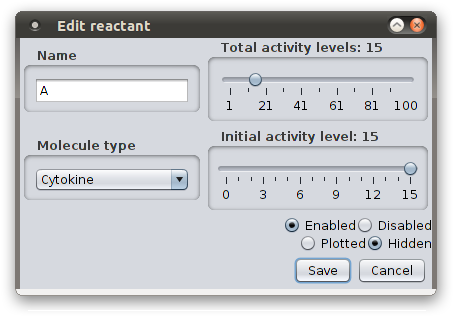
\includegraphics[width=.5\textwidth]{images/edit_reactantA}\\
 \caption{The \emph{Edit reactant} window: modifying the properties of node A.}\label{fig:edit-reactant}
\end{center}
\end{minipage}
\end{figure}


\begin{enumerate}
\setcounter{enumi}{\value{miocounterperenumerate}}
\item\label{step:add-edges} In order to add edges to the network, make sure that the \emph{Editor} tab is still active
in the \emph{Control Panel}, and
add the following edges by Ctrl-clicking the source and then clicking the target: A~$\rightarrow$~B, B~$\rightarrow$~C,
C~$\rightarrow$~B, B~$\rightarrow$~D, E~$\rightarrow$~D.
\item The \emph{Edit reaction} dialog window is opened when you add a new edge,
or when you right click an existing edge and then select the \emph{[ANIMO] Edit reaction\dots} item
from the menu. Use that window to set the parameters of the edges as indicated in Table~\ref{tab:setting-edges}. The settings
for the edge A $\rightarrow$ B should reflect the ones shown in the \emph{Edit reaction} window in Figure~\ref{fig:edit-reaction}.\\
\emph{Note}: In order to insert a qualitative parameter like the ones required by the example network,
click once the slider in the \emph{parameter} box to activate it, and then move the slider to match the requested value.
\setcounter{miocounterperenumerate}{\value{enumi}}
\end{enumerate}

\begin{table}[!ht]
\begin{minipage}{\textwidth}
\processtable{The settings for the edges (reactions) in the example.\label{tab:setting-edges}}
{\begin{tabular}{llll}%|c|c|c|c|}
\hline\noalign{\vskip 2mm}
  {\bfseries Reaction} & {\bfseries Scenario} & {\bfseries Parameter value} & {\bfseries Influence}\\[2mm]
\hline
\noalign{\vskip 2mm}  A $\rightarrow$ B & 1 & Fast & Activation\\[5mm]
\noalign{\vskip 2mm}  B $\rightarrow$ C & 1 & Medium & Activation\\[5mm]
\noalign{\vskip 2mm}  C $\rightarrow$ B & 1 & V. Fast & Inhibition\\[5mm]
\noalign{\vskip 2mm}  B $\rightarrow$ D & 1 & Medium & Activation\\[5mm]
\noalign{\vskip 2mm}  E $\rightarrow$ D & 2 & 0.00015 & Inhibition\\[2mm]
\hline
\end{tabular}}{}
\end{minipage}
\end{table}\vspace{-2ex}

\begin{figure}[!tpb]
\begin{minipage}{\textwidth}
\begin{center}
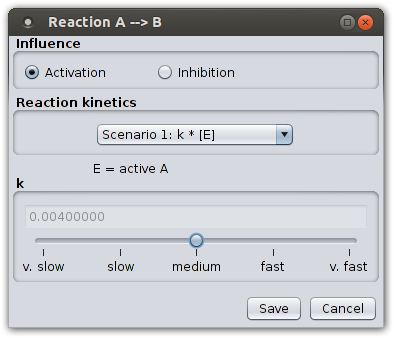
\includegraphics[width=.5\textwidth]{images/edit_reactionAB}\\
\caption{The \emph{Edit reaction} window: modifying the properties of edge A $\rightarrow$ B.}\label{fig:edit-reaction}
\end{center}
\end{minipage}
\end{figure}

\begin{enumerate}
\setcounter{enumi}{\value{miocounterperenumerate}}
\item In the \emph{Control Panel} activate the \emph{ANIMO} tab by clicking its title.
\item Click the \emph{Choose seconds/step} button. A new dialog window will appear: you can
%just click \emph{OK} to confirm that you request a time resolution of 12 seconds.
safely choose a time resolution of 12 seconds per step and click \emph{OK}.
\item Click the \emph{Analyze network} button.
\item After a few seconds the \emph{Results Panel} should appear on the right,
showing a plot of the activity level of reactant D over a time course of 240 minutes.
Figure~\ref{fig:rete-esempio} shows the resulting network and graph plot.
\end{enumerate}

\begin{figure}[!tpb]
\begin{minipage}{\textwidth}
\begin{center}
  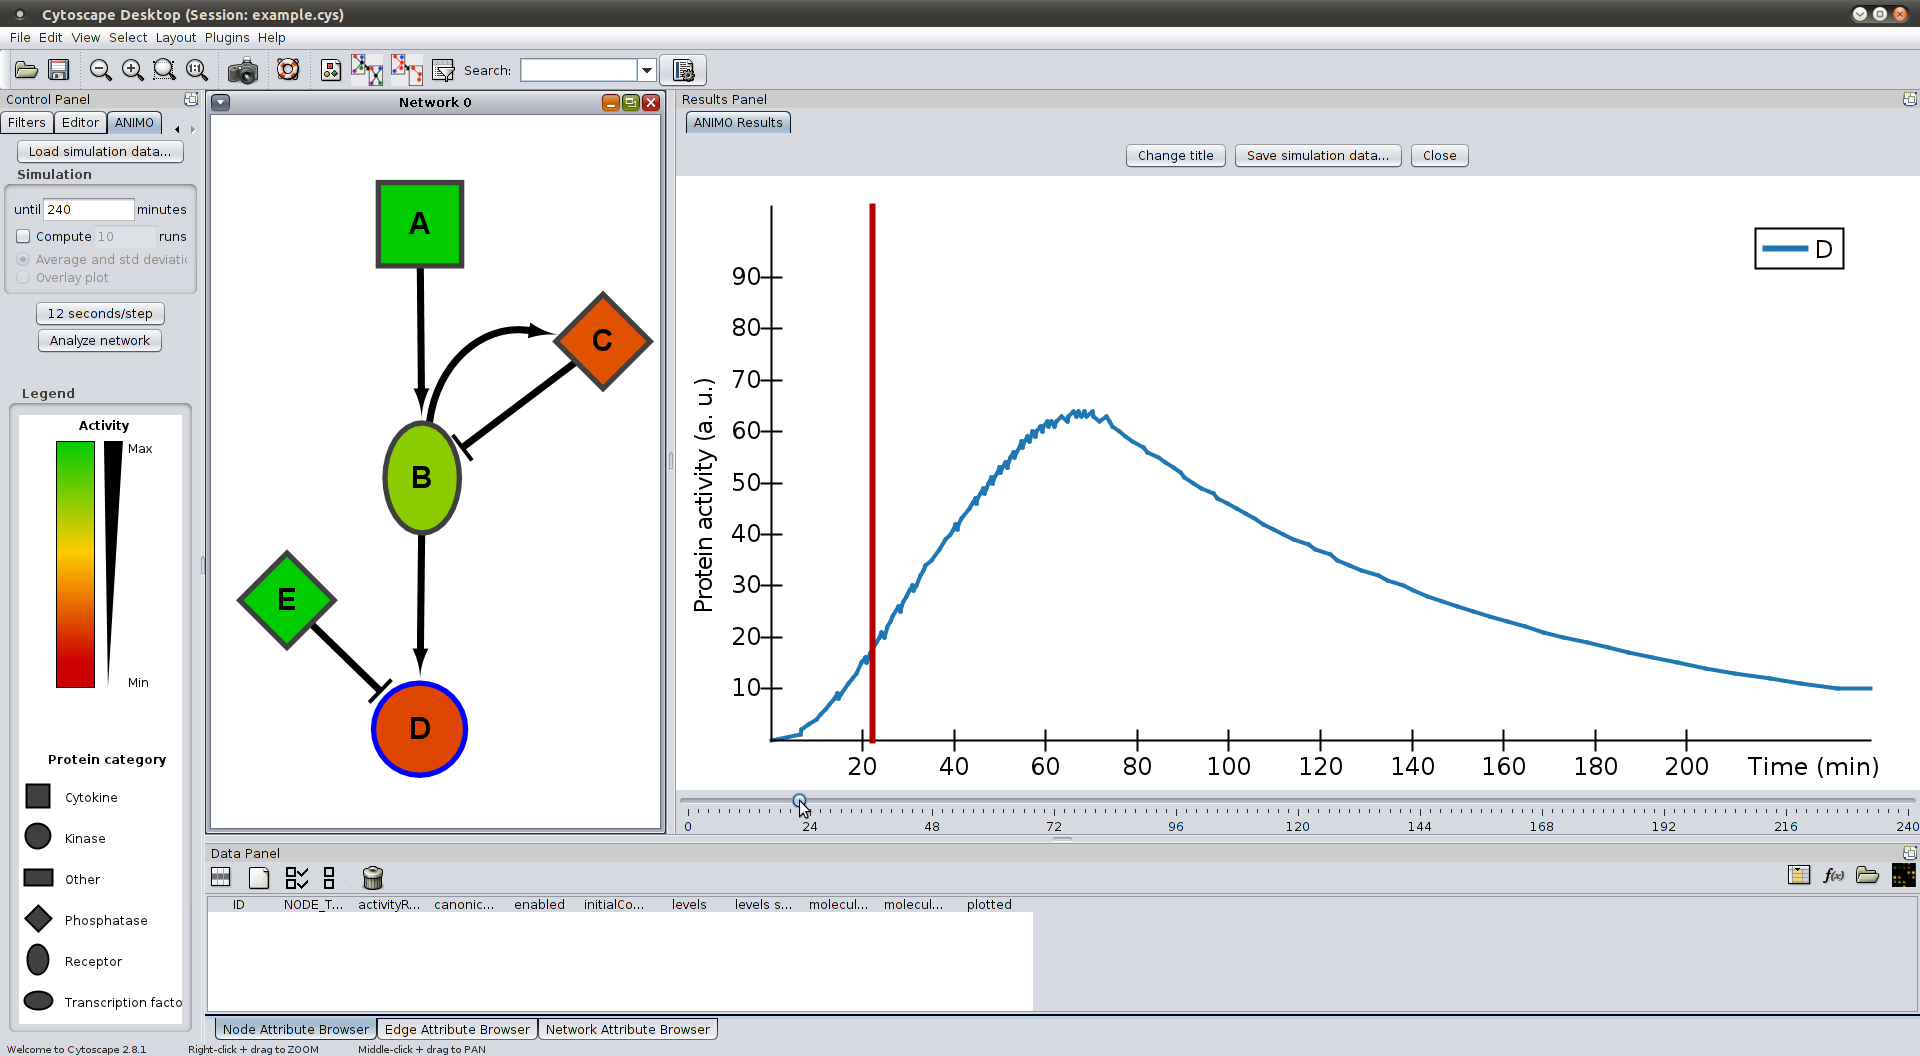
\includegraphics[width=.9\textheight, angle=90]{images/esempio_uso_ANIMO3}
\end{center}
\caption{The completed example, where also the feature that allows to view the activity levels
of reactants at chosen simulation times is demonstrated: the vertical red bar in the graph on the
right can be moved through the slider under the graph, and indicates the point in the time series
on which the coloring of the nodes in the \emph{Network} window is based.
The legends for colors and shapes can be found in the \emph{Legend} panel.}\label{fig:rete-esempio}
\end{minipage}
\end{figure}


\subsubsection{Managing simulation data and activity levels plots}
Each time a simulation result is obtained, a new tab is added to the \emph{Results Panel} (see the right part of Fig.~\ref{fig:rete-esempio})
in which we identify three buttons, a plot of the activity levels of the selected reactants and a time slider.

Clicking on the button \emph{Change title} allows to select a new title for the tab: this can be useful e.g. when comparing different
simulations made on similar configurations of the same network. Button \emph{Save simulation data\dots} allows to save
the simulation data of the current tab on a \emph{.sim} file, which can then be loaded and inspected in the future.
The \emph{Load simulation data\dots} button in the \emph{Control Panel} above the \emph{Simulation} box can be used for this purpose.
Please note that the best results are obtained only when loading a \emph{.sim} file when the \emph{Network} window contains the same network
on which the simulation data are based. If no network is currently opened, a network will \emph{not} be opened by loading a \emph{.sim} file.
The \emph{Close} button is used to close the currently displayed results tab.

Right clicking inside the graph area will bring up a menu that allows to perform some basic operations with the graph
and its data:
\begin{itemize}
  \item \emph{Add data from CSV}: superpose the graph with other data series found in a \emph{.csv} (comma separated values) file. This file type can be
obtained for example by exporting data from the default Excel format. If you want the data in the \emph{.csv} file to be rescaled so
that its maximum Y value coincides with the maximum in the plot, the data file needs to contain a column named (exactly)
\emph{Number\_{}of\_{}levels}, on the first row of which the maximum of the scale for the \emph{.csv} data needs to be put. For example,
if the data in the \emph{.csv} file are on a 0-100 scale, the value for \emph{Number\_{}of\_{}levels} will be 100.
  \item \emph{Save as PNG}: save the graph as it is shown in a \emph{.png} image file. This file format can be opened by most
image editors.
  \item \emph{Export visible as CSV}: export to a \emph{.csv} file all the series that are currently visible (i.e., not hidden)
in the graph.
  \item \emph{Clear Data}: clear the contents of the graph, removing all series. This can be useful for plotting
a \emph{.csv} file without superposing it to the current graph, or for loading a file in which all hidden data where removed
(exporting the visible graph to a \emph{.csv} with the previous command).
  \item \emph{Graph interval}: change the lower and upper bounds for X and Y axes.
  \item \emph{Zoom rectangle}: zoom the graph around a user-chosen rectangular area.
    After selecting this command the shape of the mouse cursor changes into a cross. The area of the plot to be
    zoomed can then be selected by dragging a rectangular selection around it (see the definition of \emph{rectangular
    selection} on page~\pageref{nota:rectangular-selection}).
  \item \emph{Zoom extents}: bring the zoom level back to default, canceling the effects of any \emph{Zoom rectangle}
command.
\end{itemize}

Whenever the result of one or more simulations is shown as a graph, it is possible to use the slider under the graph to
move through the entire simulation, showing the activity levels of all reactants represented with different node coloring in
the \emph{Network} window on the left. For an example, see Figure~\ref{fig:rete-esempio}: the vertical red line in the
graph represents the time instant on which the colors of the nodes in the \emph{Network} window are based, and can
be moved with the slider over which the mouse cursor is drawn.




\subsection{Additional tips}
\subsubsection{Editing a network in Cytoscape}
Nodes and arcs can be placed in the network as shown previously: with the \emph{Editor} tab selected in the
\emph{Control Panel},
Ctrl-click (click while holding the {\tt Ctrl} or \maccmd\ key) in an empty place to add a node; Ctrl-click the source
node and click the target node to add an arc. It is also possible to drag and drop the node/arc icons from the \emph{Control Panel}
into the \emph{Network} window.\\
\emph{Note}: to perform \emph{drag and drop} move the mouse cursor over the icon in the \emph{Control Panel}, click with the left mouse
button and, without releasing the button, drag the mouse cursor on the \emph{Network} window where you want to
place the symbol; then release the left mouse button.

In order to delete a node/edge, select it by clicking
or grouping them in a larger rectangular selection, and then press the \emph{Delete} key on the keyboard
or select the \emph{Edit} $\rightarrow$ \emph{Delete Selected Nodes and Edges} menu command.\\
\emph{Note}: in order to obtain a \emph{rectangular selection}\label{nota:rectangular-selection},
left click in the \emph{Network} window where the upper-left corner of the rectangle should be and,
without releasing the left mouse button, drag the mouse cursor to where the lower-right corner of the
rectangular selection should be; then release the left mouse button. All the entities which were
\emph{even partially} touched by the rectangle are now selected.

Navigation inside the \emph{Network} window can be performed by clicking and dragging the center mouse button,
while zooming can be done by either rotating the mouse wheel or clicking and holding the right mouse button
while moving the mouse in a vertical direction.

Finally, note that the colors used to represent node activity can be changed using the \emph{VizMapper}
interface provided by Cytoscape, changing the setting for \emph{Node color}, shown in Figure~\ref{fig:change-gradient}.
To change the node colors, activate the \emph{VizMapper\texttrademark} tab in the \emph{Control Panel}, and
find the entry named \emph{Node Color} in the \emph{Visual Mapping Browser} box. Click the arrow-shaped
icon directly to the left of \emph{Node Color}: the current setting for the node colors should appear:
click the colored bar to open the window shown in Figure~\ref{fig:change-gradient}.
The \emph{activityRatio} on which the node coloring is based is the ratio between the current activity level
of a node and its number of activity levels.
The colored arrows pointing downward on the upper border of the colored rectangle can be dragged along the length of the $[0, 1]$
interval, thus changing the point at which a particular color appears. New arrows can be added with the \emph{Add} button, while
clicking an arrow and pressing the \emph{Delete} button will remove one. To change the color of a point in the interval,
double click the corresponding arrow, and a new window will open, allowing you to choose a new color: clicking \emph{OK} will
accept the new color. The modifications made in the \emph{Gradient Editor for Node Color} window should be automatically reflected in
the model: when the gradient is as wanted, simply close the window. If the node colors seem not to have been updated, please move the
slider under an existing graph in the \emph{Results Panel}.

\begin{figure}[!tpb]
\begin{minipage}{\textwidth}
\centering
  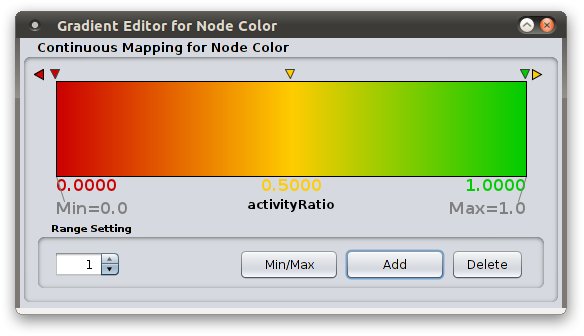
\includegraphics[width=.6\textwidth]{images/editing-gradient2}
  \caption{Changing the colors used to represent node activity in an ANIMO model.}\label{fig:change-gradient}
\end{minipage}
\end{figure}


\subsubsection{ANIMO features}
Nodes and edges (and groups of nodes/edges highlighted via a rectangular selection)
can be disabled by choosing \emph{[ANIMO] Enable/disable} from
the right-click menu: they will be represented with less saturated colors and can be re-enabled by performing
the same action. Moreover, a node can be enabled/disabled directly in its properties window, where it is
also possible to add/remove the node from the list of series appearing in the graph resulting from a simulation
of the network by selecting \emph{Plotted} or \emph{Hidden} (see also Figure~\ref{fig:edit-reactant}):
nodes that will be plotted are circled in blue.
Every enabled node will be taken into account when computing the evolution of the system,
but only nodes marked as \emph{Plotted} will appear in a graph.

Each plot in an \emph{ANIMO Results} tab contains by default a legend, which can be used to modify which series are
displayed and how they are displayed. Clicking with the central mouse button on a series name will hide it from the
graph, while the same center-click the colored line beside the series name will change the color of that series,
cycling through a predefined set of available colors. The entire legend can be hidden by clicking with the
central mouse button anywhere on the graph (not inside the legend), or it can be dragged around by clicking and holding the left
mouse button, releasing it when the preferred position is reached. Rotating the mouse wheel will allow the thickness of all
the graph lines, and the size of the text, to grow or decrease: this feature can be useful when the window containing
the graph is very large.

As the model is non-deterministic, i.e. its
evolution will not be exactly the same for every single simulation run, it is possible to ask ANIMO to perform
a number of simulation runs in a batch, plotting the averages of the activity levels over the runs together with a standard
deviation value, or showing a so-called \emph{overlay plot} where all runs are plotted over each other. The controls
that allow to ask for multiple simulation runs can be found in the \emph{Control Panel}, inside the \emph{Simulation} box.

Standard deviation may be represented in the graph: it is normally shown as vertical bars, but its aspect can be
cycled through five possibilities (vertical bars, shading, both bars and shading, bars and symbols, none) by right-clicking the
corresponding line in the legend. Symbols associated to a representation of standard deviation can be changed by Shift-right-clicking
(holding down the \emph{Shift} key, right click) on the corresponding line in the legend.
Standard deviation values can be obtained when asking for multiple simulations in the network
analysis, but they can also be present in a \emph{.csv} file, e.g. when the file contains averages of experimental data.
In a \emph{.csv} file, the column containing the standard deviation values for column \emph{A}
should be named \emph{A\_{}StdDev} for the program to recognize it and properly display the data series
with the associated error values.



\subsubsection{Parameter settings}
The application of some basic strategies when setting the parameters for a network allows
the less experienced users to considerably shorten the modeling time.
First of all, it is important to proceed in a \emph{top-to-bottom} order, trying to match
a component to the corresponding data before inserting the components downstream thereof.
Second, when choosing the kinetic parameter for a reaction, we advise to first use the qualitative settings (very slow, slow, medium, fast, very fast):
this allows to define the relative speeds of the reactions as soon as possible,
leaving the more precise parameter setting procedure as a follow-up step. Finally, as can be seen from
the parameter settings of Section~\ref{sec:modeling-network-example}, in order to obtain a peak
behavior it is particularly important that
a negative feedback is present (as an example, see the reactions involving B and C in Tab.~\ref{tab:setting-edges}),
and that the inactivating reaction in the loop is faster than the ones activating the target node.

A final note on the \emph{seconds/step} button. This button allows to define the time granularity
of the simulations, but it is not strictly necessary to choose a very precise value.
% As the time bounds in the \tas\ model are integers, rounding errors can make the model
% behave differently from what the parameters define.
If the current value for \emph{seconds/step}
is too high (or too low) to allow the network to be properly simulated, ANIMO will automatically choose (respectively)
the highest (lowest) value that still allows to avoid rounding problems. It will be possible to notice
such a change in the value of time scale when the number on the \emph{seconds/step} button changes.


\subsubsection{Updating ANIMO}
To check whether a new version of ANIMO has been published, run Cytoscape and ask for an update of all
plug-ins via the menu command \emph{Plugins} $\rightarrow$ \emph{Update Plugins}. After some seconds
during which Cytoscape will contact all the providers of the installed plug-ins,
the system should report the list of updatable plug-ins.\\
\emph{Note}: a window with the message \emph{Attempting to connect to XYZ\dots} may appear and disappear multiple times:
it is the normal behavior.

If an updated version of ANIMO is available, it will appear
under the category \emph{Updatable Plugins} $\rightarrow$
\emph{Analysis} $\rightarrow$ \emph{ANIMO v1.28}. If no plug-in can be updated, a message stating \emph{No
updates available for currently installed plug-ins.} will be shown.








\clearpage
\section{Additional notes}

\subsection{Simulating the day-night cycle}\label{suppl:repressilator}
The model presented in Figure~\ref{subfig:drosophila-model} contains a node
labelled {\sf Day/Night}. That node abstracts our representation
of the cyclic alternance of day and night, which causes the variations
in cryptochrome ({\sf cry}): these oscillations allow the network
to synchronize to a time zone. Note that the network oscillates
also when the node {\sf cry} is not included in the model.

The alternance between day and night is represented in our model with a
repressilator-like~\citep{repressilator} subnetwork, as can be seen in Figure~\ref{fig:repressilator}.
In the model by~\cite{drosophila-ode-model} a specific function
was introduced in the equations to approximate the experimental data from~\cite{drosophila-cry-data}.

\begin{figure}[!htb]
\begin{minipage}{\textwidth}
  \centering
  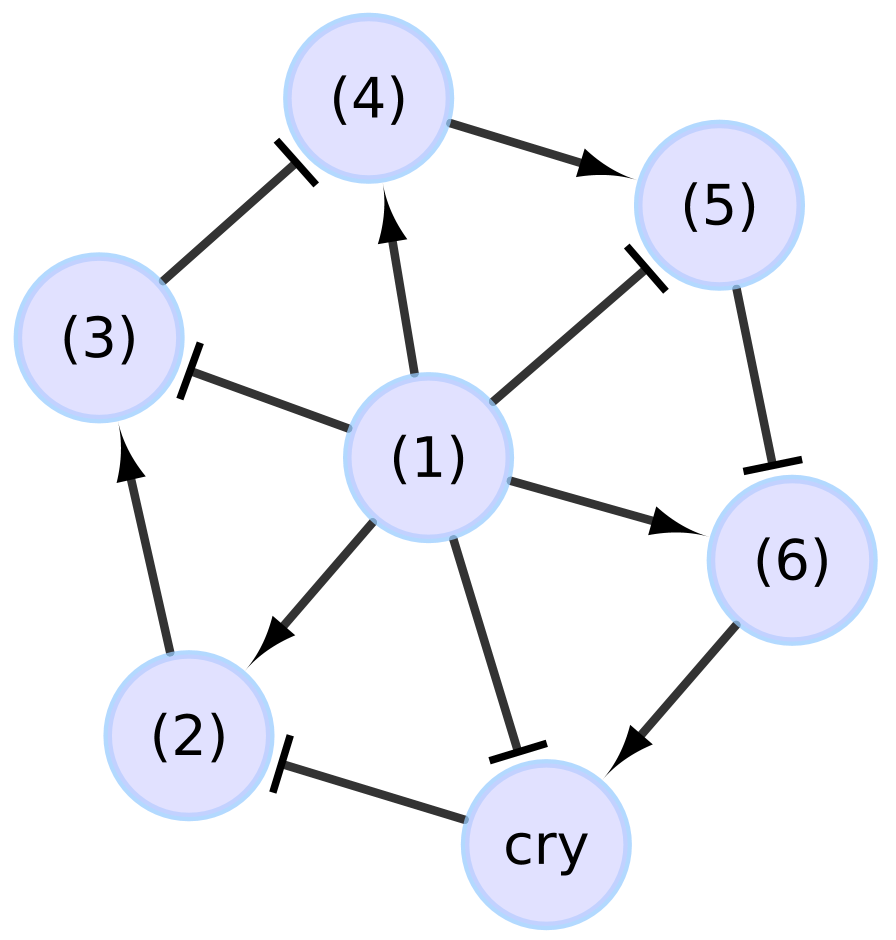
\includegraphics[width=0.35\textwidth]{images/drosophila_model_repressilator}
\caption{The repressilator-like subnetwork used to represent the alternance
between day and night that cause the oscillations in {\sf cry} concentrations in the
network modelled in Section~\ref{sec:animo-drosophila}.}\label{fig:repressilator}
\end{minipage}
\end{figure}



\subsection{Note on the parameters in the TNF$\alpha$-EGF model}\label{suppl:parameters-tnf-egf}
The parameters in the model in Figure~\ref{fig:large-model-complete}
have been set by fitting the model to the experimental data for conditions with 100 ng/ml TNF$\alpha$.
In the model we have set the starting level of TNF$\alpha$ at 100 out of 100 for these conditions.
This level is a dimensionless quantity that indicates the maximum activity level in the data set.
We found that setting the initial level of TNF$\alpha$ at level 8 out of 100 gave slightly better results for the
condition with 5 ng/ml TNF$\alpha$ than level 5 out of 100. We believe that this has to do with the fact that
100 ng/ml is a highly supra-physiological concentration of TNF$\alpha$, that will rapidly cause activation of all
receptors present. Fitting the model to this experimental condition may have resulted in slight deviations
in the parameter values. Nevertheless, the modeling results illustrate that building a model with basic
kinetic rate laws can give useful predictions over a range of concentrations. Figures~\ref{fig:large-model-graph3} and~\ref{fig:large-model-graph4}
show the modeling results with TNF set at 8 out of 100.

\clearpage
\section{How ANIMO uses Timed Automata to model pathway dynamics}\label{suppl-sec:animo-ta}


% \subsection{From biochemical reactions to activity-based interactions}
% ANIMO models are based on the concept of \emph{activity level},
% which is a discrete representation of the active fraction of a molecular species.
% We consider a molecule to be \emph{active} when it has undergone a modification
% that entails a new function: e.g. a phosphorylated kinase is usually considered
% active. Each node in an ANIMO model represents a molecular species,
% and its color is determined by the current activity level of the species.
% Biochemical reactions are represented as
% abstract interactions similarly to the traditional representation of signaling networks.



% \subsection{From interactions to Timed Automata}\label{subsec:timed-automata}
% \def\ta{TA}
% \def\tas{TA}
% A Timed Automaton (\ta) consists of states and transitions between these states (Figs.~\ref{subfig:erk}, \ref{subfig:mek}).
% Each automaton has local clocks associated to it that allow to control residence in its states, and transitions between states.
% Communication channels enable synchronization of transitions in different automata. The synchronization between two
% automata on channel $c$ requires one automaton to send a message: $c!$ while the other automaton performs the
% corresponding action: $c?$ to receive the message. A simplified \tas\ model of the activation of extracellular
% regulated kinase (ERK) by MAPK ERK kinase (MEK) illustrates these basic properties of \tas\
% (Fig.~\ref{fig:abstraction-mek-erk}). In this example, MEK activity is not regulated and ERK has only two activity levels,
% completely inactive or completely active. In the network visualization, each molecular species (e.g. ERK) is depicted as a single node,
% colored according to its activity (Fig.~\ref{subfig:mek-erk}).
%
%
%
%
% \def\mekTA{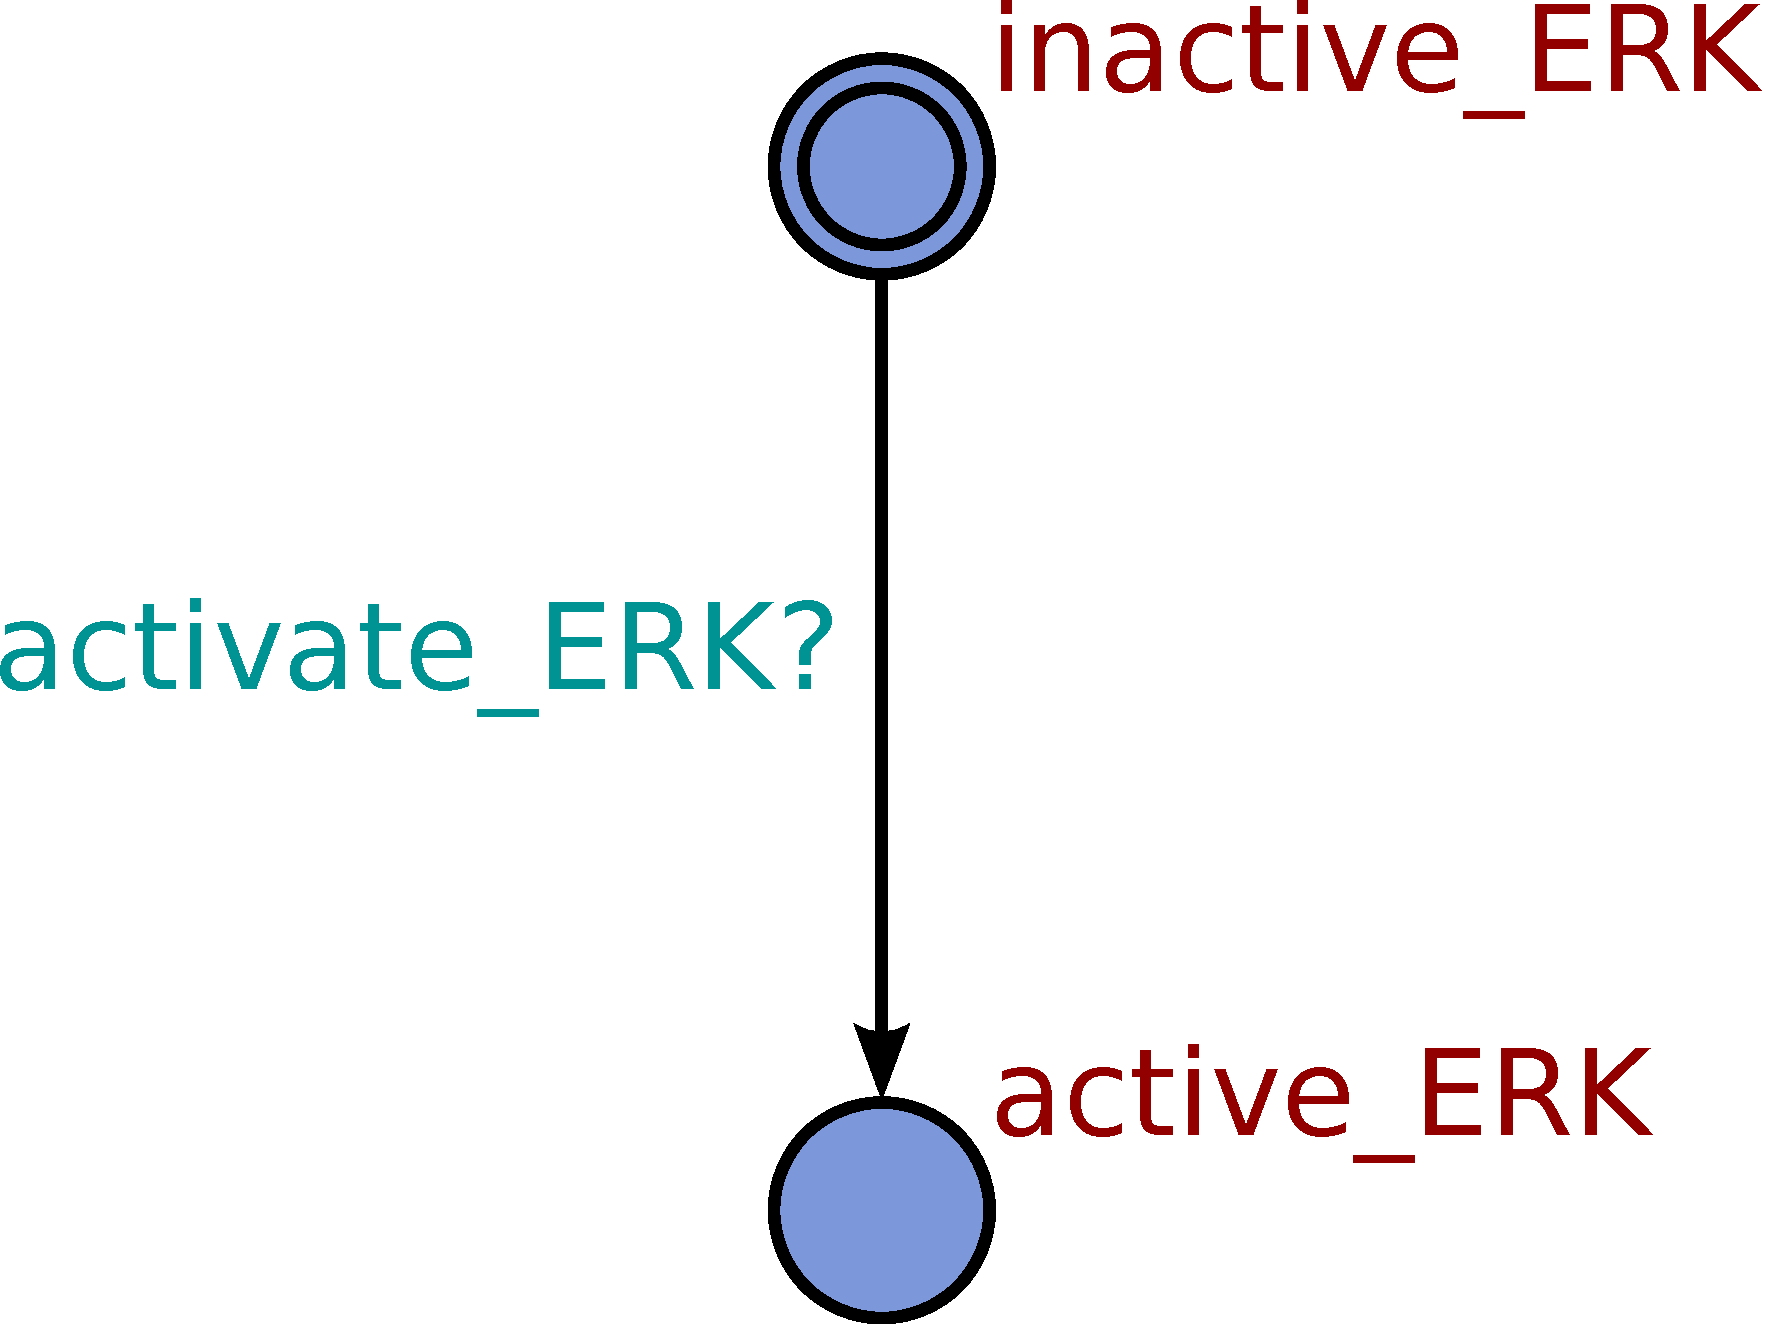
\includegraphics[scale=.098]{images/abstraction_ta_erk}}
% \newlength\mekTAheight
% \setlength\mekTAheight{\heightof{\mekTA}}
% \begin{figure}[!hb]
% \begin{minipage}{\textwidth}
% \begin{center}
% \subfloat[\label{subfig:mek-erk}]{\begin{minipage}[c][\mekTAheight]{0.13\textwidth}\begin{center}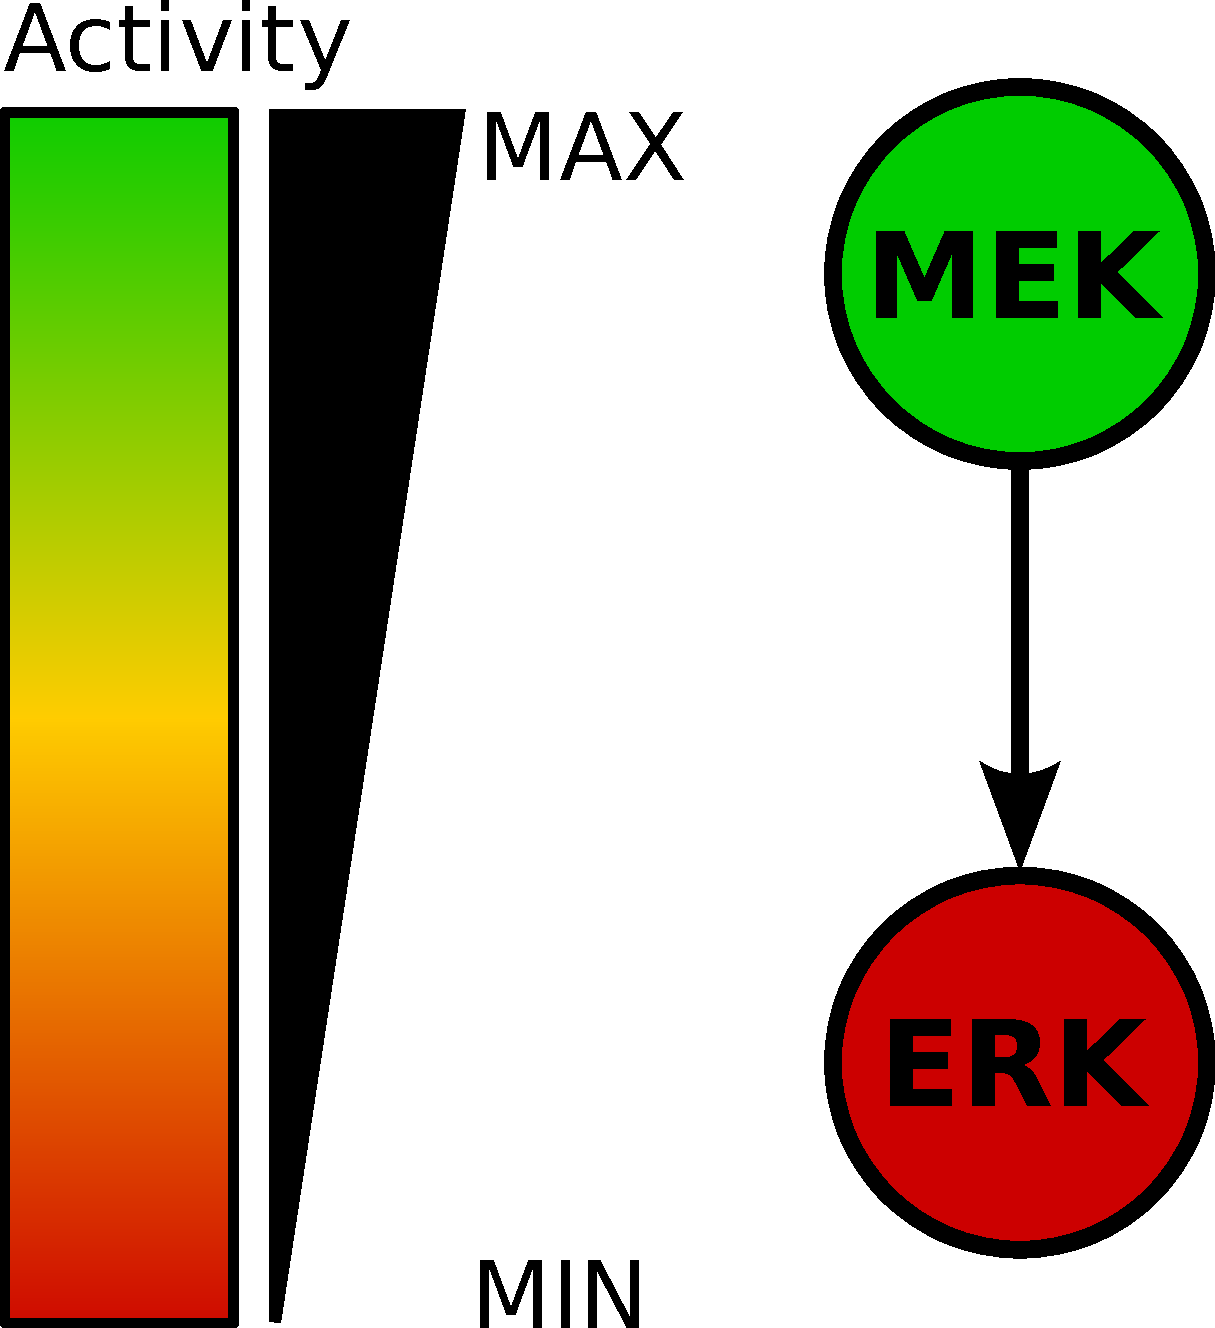
\includegraphics[scale=.098]{images/abstraction_ta_mek-erk3}\end{center}\end{minipage}}
% \ \
% \subfloat[\label{subfig:erk}]{\begin{minipage}[c][\mekTAheight]{0.18\textwidth}\begin{center}\mekTA\end{center}\end{minipage}}
% \ \
% \subfloat[\label{subfig:mek}]{\begin{minipage}[c][\mekTAheight]{0.14\textwidth}\begin{center}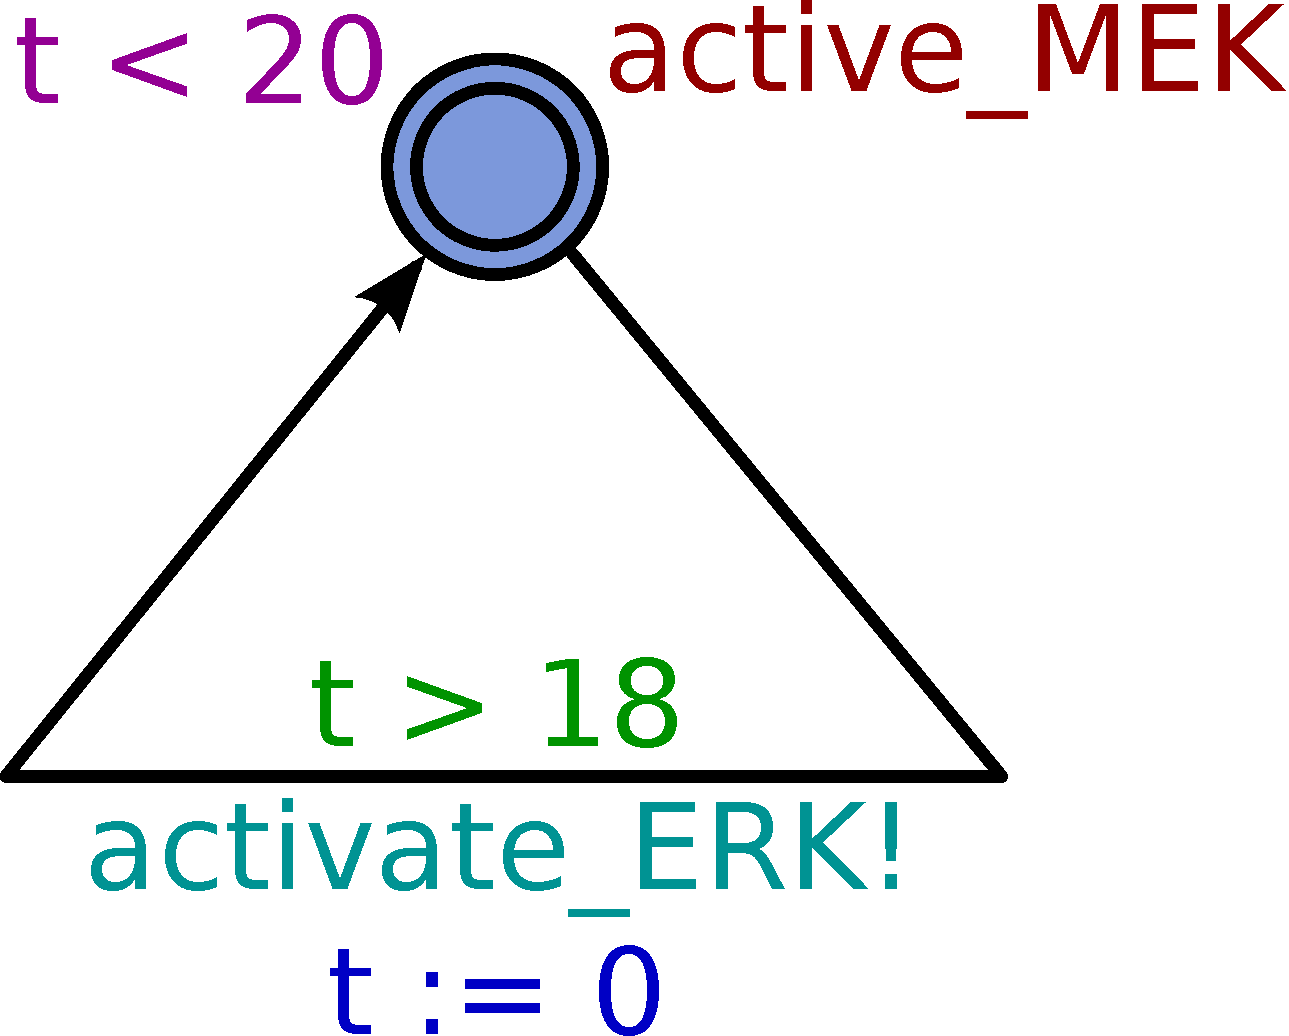
\includegraphics[scale=.098]{images/abstraction_ta_mek}\end{center}\end{minipage}}
% \end{center}
% \caption{Abstraction of a biochemical reaction to a \tas\ model.
% {\bf \protect\subref{subfig:mek-erk}}~Classical depiction of a well-studied intracellular signal transduction reaction: protein
% MAPK-ERK kinase (MEK) activates downstream protein extracellular-regulated kinase (ERK).
% {\bf \protect\subref{subfig:erk}}~A \ta\ model of ERK, consisting of two states (circles), {\sf inactive\_ERK} and {\sf active\_ERK},
% and one transition (arrow) between the states. This transition will take place when it is possible to synchronize with
% the corresponding action {\sf activate\_ERK!} in the MEK automaton.
% {\bf \protect\subref{subfig:mek}}~A \ta\ model of active MEK, consisting of one state and one
% transition. ${\sf t} < 20$ is termed an invariant on the state, allowing residence in this state as long as local
% clock time {\sf t} is smaller than $20$ units. ${\sf t} > 18$ is termed a guard on the transition, allowing the
% transition to take place when local clock {\sf t} is greater than $18$ units. Together, the invariant and guard in this
% example ensure that the transition must take place in the (continuous) time interval $18 < {\sf t} < 20$. When the
% transition takes place, the action {\sf activate\_Erk!} is performed (thus allowing the ERK automaton to reach the {\sf
% active\_ERK} state) and the local clock coupled to this automaton is reset, ${\sf t} := 0$.}\label{fig:abstraction-mek-erk}
% \end{minipage}
% \end{figure}
%
%
% When building an ANIMO model, the user can choose the number of discrete activity levels for each node, ranging
% between 2 and 100, depending for example on the quality of experimental data.
% Coarse-grained models have a low number of activity levels and are less precise,
% whereas fine-grained models have a higher number of activity levels and behave more like continuous models (see Fig.~\ref{fig:levels}).
%
% Variable reaction rates are accounted for by having variable time constraints to transitions, fast
% reactions being reflected by small time values. These values depend on the current activity level of the involved reactants.
% Using basic kinetic rate laws, time constraints are pre-computed for all possible activity levels and stored in a pair of tables.
% When the activity level of one of the input variables to a reaction changes, the tables are used to
% update the reaction rates for all reactions involving this reactant (see Fig.~\ref{fig:ta-diagram}).
% A more detailed account on the \tas\ model underlying ANIMO can be found in Suppl. Sect.~\ref{suppl-sec:animo-ta}.






\subsection{Timed Automata model}
The Timed Automata (\tas) model underlying an ANIMO network is generated whenever an analysis is requested by the user.
Starting from the network represented in the Cytoscape-based user interface, ANIMO automatically generates a \tas\ model
to be used with UPPAAL. The analysis result is then parsed and properly represented to the user, for example
as a graph of reactant activity levels.

The behavior of all reactions in an ANIMO model is based on the same \ta\ template: Figure~\ref{fig:ta-model-simpler}
shows UPPAAL's graphical representation of such template. An instance of the reaction template is generated for each
of the reactions present in the ANIMO model, and is equipped with a local clock {\sf c} to measure the time until
the next reaction step. Moreover, a global clock is defined for the whole model, to keep track of the current experiment time
in a simulation. To represent the activity level of the molecular species included in the ANIMO model, each
reactant R is associated to an integer variable {\sf R}.
The automaton in Figure~\ref{fig:ta-model-simpler} uses {\sf MEK} to refer to the activity level of MEK, from which the reaction speed depends.
The initial activity level of each node is chosen by the user when modifying the node
in the ANIMO model: these settings define the starting state for the \tas\ model.
Each reactant R is also associated to a channel named {\sf R\_reacting}, which is
used to communicate between automata when the activity level of a reactant is changed.



\tikzstyle{decision} = [rectangle, draw, fill=yellow!20, text width=.45\textwidth, text badly centered]
\tikzstyle{block} = [rectangle, draw, fill=blue!20,
    text width=.45\textwidth, text centered, rounded corners, minimum height=4em]
\tikzstyle{line} = [draw, thick, -latex']
\tikzstyle{cloud} = [draw, ellipse,fill=blue!20, minimum height=2em]
\def\svgwidth{.8\textwidth}
\definecolor{lowActivity}{rgb}{0.8,0,0}
\definecolor{highActivity}{rgb}{0,0.8,0}%{1,0.8,0}
\newsavebox{\mysquareLow}
\savebox{\mysquareLow}{%
  \raisebox{-0.08em}{%
    \textcolor{black}{%
      \rule{.7em}{.7em}%
    }%
    \hspace{-.65em}%
    \raisebox{.05em}{%
      \textcolor{lowActivity}{%
	\rule{.6em}{.6em}%
      }%
    }%
  }%
}
\newsavebox{\mysquareHigh}
\savebox{\mysquareHigh}{%
  \raisebox{-0.08em}{%
    \textcolor{black}{%
      \rule{.7em}{.7em}%
    }%
    \hspace{-.65em}%
    \raisebox{.05em}{%
      \textcolor{highActivity}{%
	\rule{.6em}{.6em}%
      }%
    }%
  }%
}

\begin{figure}[!ht]
\begin{minipage}{\textwidth}
\centering

\begin{tikzpicture}[node distance = 2cm, auto, scale=0.8, every node/.style={scale=0.8}]
    % Place nodes
    \node [block] (init) {
\begingroup
  \makeatletter
  \providecommand\color[2][]{%
    \errmessage{(Inkscape) Color is used for the text in Inkscape, but the package 'color.sty' is not loaded}
    \renewcommand\color[2][]{}%
  }
  \providecommand\transparent[1]{%
    \errmessage{(Inkscape) Transparency is used (non-zero) for the text in Inkscape, but the package 'transparent.sty'
is not loaded}
    \renewcommand\transparent[1]{}%
  }
  \providecommand\rotatebox[2]{#2}
  \ifx\svgwidth\undefined
    \setlength{\unitlength}{1974.66679688pt}
  \else
    \setlength{\unitlength}{\svgwidth}
  \fi
  \global\let\svgwidth\undefined
  \makeatother
  \begin{picture}(1,0.37)%26031697)%
    \put(0,0){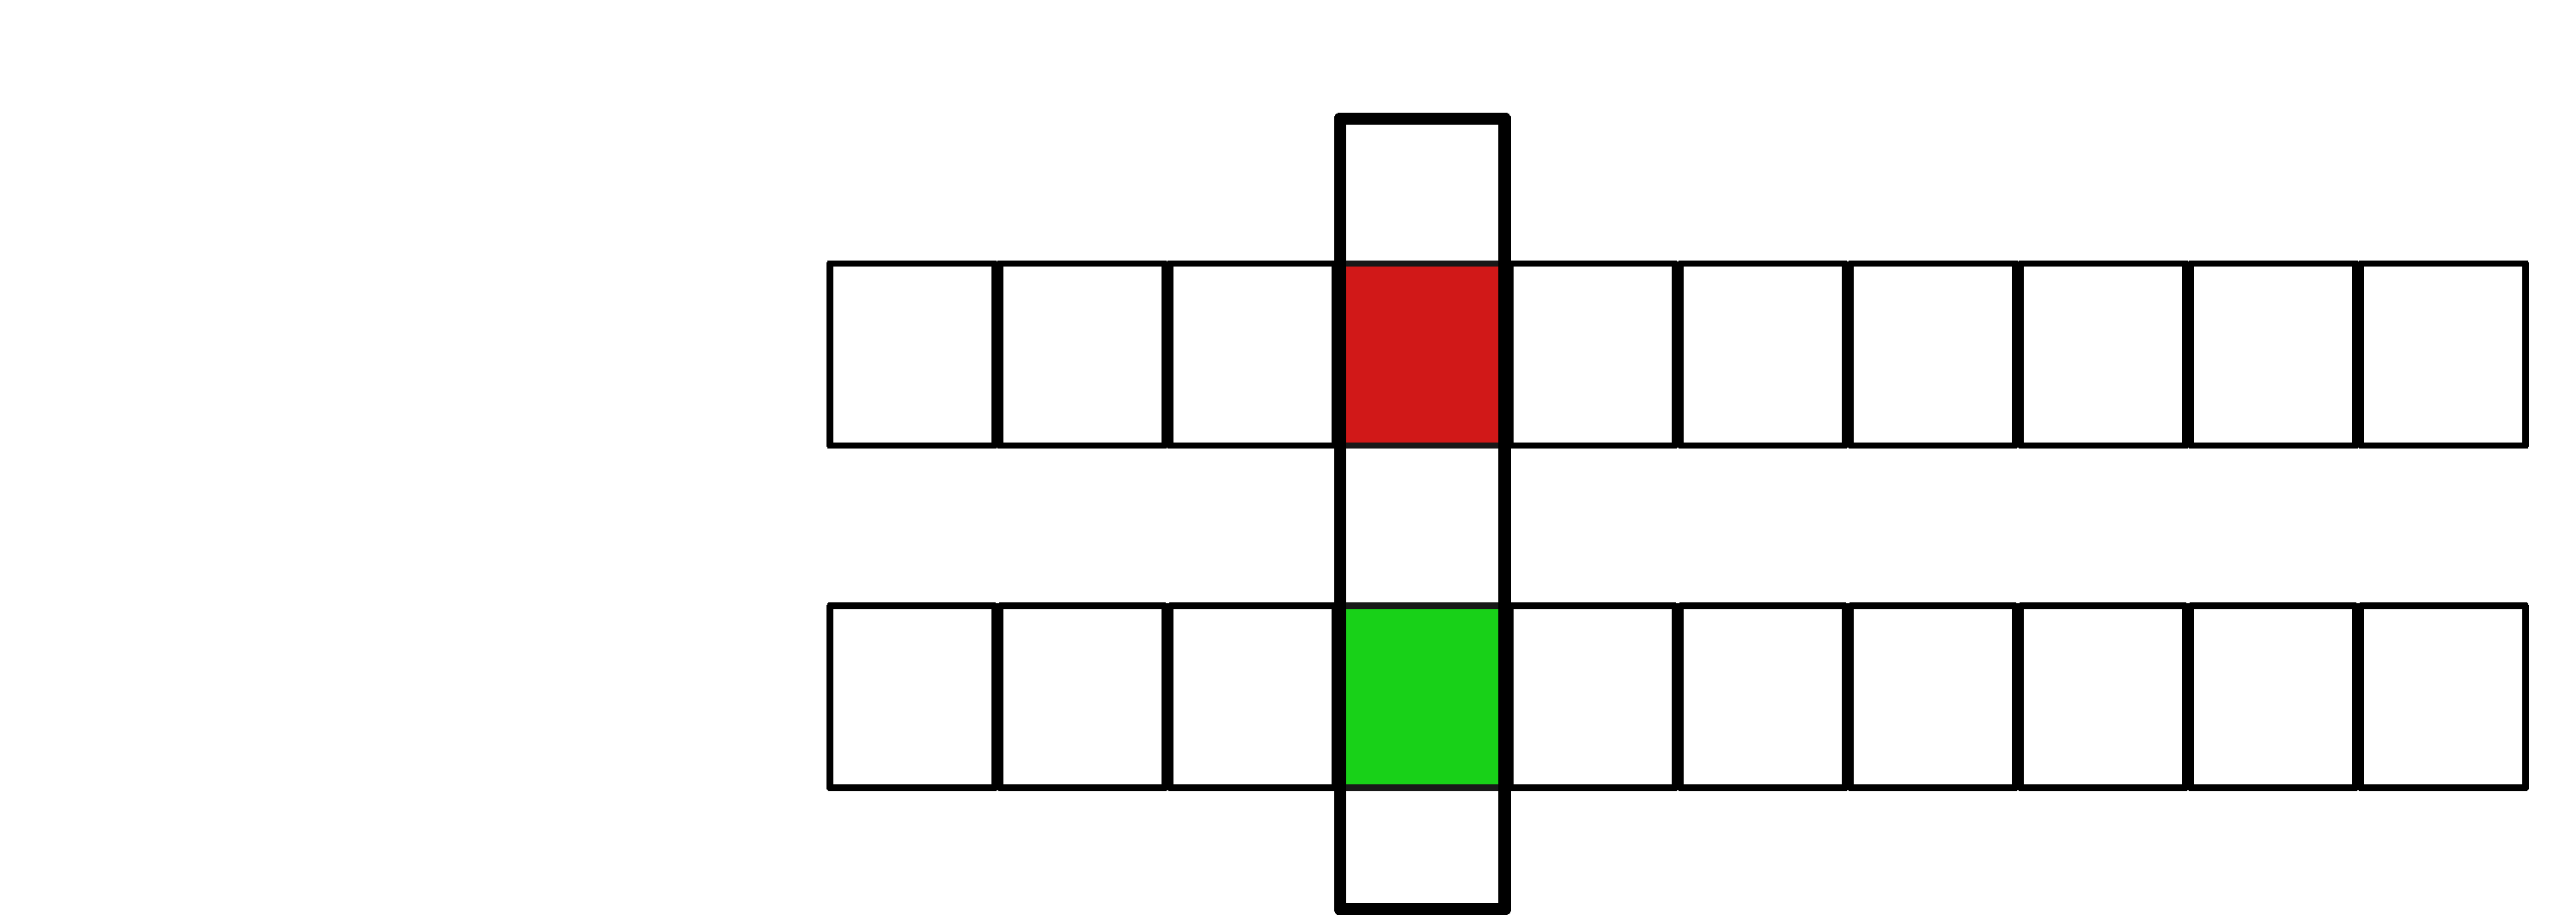
\includegraphics[width=\unitlength]{images/mek_activity_time_tables2.pdf}}%
    \put(0.02042129,0.20182345){\color[rgb]{0,0,0}\makebox(0,0)[lb]{\smash{$R_{\mbox{\scriptsize lowerBound}}$}}}%
    \put(0.02042129,0.07442319){\color[rgb]{0,0,0}\makebox(0,0)[lb]{\smash{$R_{\mbox{\scriptsize upperBound}}$}}}%
    \put(0.45,0.325)%23815501)
	{\color[rgb]{0,0,0}\makebox(0,0)[lb]{\smash{$\mbox{MEK}_{\mbox{\scriptsize
activity}}$}}}%
  \end{picture}%
\endgroup
};
    \node [block, above of=init, node distance=2.5cm] (reset) {Reset the internal clock: ${\sf t} \!\!:= \!\!0$};
    \node [cloud, above of=reset, node distance=1.5cm] (start) {Start};
\node [block, below of=init, node distance=2.5cm] (choose) {$R$ will occur when
\raisebox{-0.3ex}{\pgfuseimage{lower-bound}} $\leq\!\!\! {\sf t}\!\!\! \leq$
\raisebox{-0.3ex}{\pgfuseimage{upper-bound}}
    };
    \node [block, below of=choose] (increase) {Increase $\mbox{ERK}_{\mbox{\scriptsize activity}}$
by $+1$ level};
    \node [block, below of=increase] (inform) {Inform reactions depending on $\mbox{ERK}_{\mbox{\scriptsize
activity}}$\\
    of the change};
    % Draw edges
    \path [line] (start) -- (reset);
    \path [line] (reset) -- (init);
    \path [line] (init) -- (choose);
    \path [line] (choose.west) -| +(-0.5, 2) node [pos=0.78, sloped, above, align=left] {$\mbox{MEK}_{\mbox{\scriptsize activity}}$ was changed} |- (init.west);
    \path [line] (choose) -- (increase);
    \path [line] (increase) -- (inform);
    \path [line] (inform.east) -| +(1, 4) |- (reset.east);
\end{tikzpicture}
\caption{Schematic overview of the steps taken during a simulation run by a Timed Automaton modeling a reaction $R$ that increases $\mbox{ERK}_{\mbox{\scriptsize activity}}$ and depends only on $\mbox{MEK}_{\mbox{\scriptsize activity}}$.
In this example, MEK has 10 activity levels. After resetting the internal clock {\sf t}, the automaton sets the time constraints for the reaction.
$\mbox{MEK}_{\mbox{\scriptsize activity}}$ is used as the index inside the time
tables $R_{\mbox{\scriptsize lowerBound}}$ and $R_{\mbox{\scriptsize upperBound}}$.
Once the bounds have been identified, %the internal clock {\sf t} begins counting.
$R$ can occur when {\sf t} reaches a value
inside the continuous time interval~$[\,\usebox{\mysquareLow}, \usebox{\mysquareHigh}\,]$. When it occurs, $R$ increases the value of
$\mbox{ERK}_{\mbox{\scriptsize activity}}$ by $1$. All reactions that depend on
$\mbox{ERK}_{\mbox{\scriptsize activity}}$ are notified of the change, and the associated time bounds are updated accordingly.
After resetting the clock {\sf t}, the reaction process can restart.
If $\mbox{MEK}_{\mbox{\scriptsize activity}}$ was changed by another reaction before the occurrence of $R$, the automaton needs to update the correct
time bounds based on the new activity level of MEK.}\label{fig:ta-diagram}
\end{minipage}
\end{figure}



The abstract behavior of a reaction in the \tas\ model is described in Figure~\ref{fig:ta-diagram}:
after choosing the correct time bounds, the automaton waits for the reaction to complete, then updates the values of the output variable
and is ready to restart.
If an intervening event has changed the value of a reactant from which the reaction time bounds depend, the
bounds are updated at run-time. Referring to the \ta\ template in Figure~\ref{fig:ta-model-simpler},
we will now give a less abstract description of the behavior of the formal model.


\begin{figure}[htpb]
\begin{minipage}{\textwidth}
  \centering
  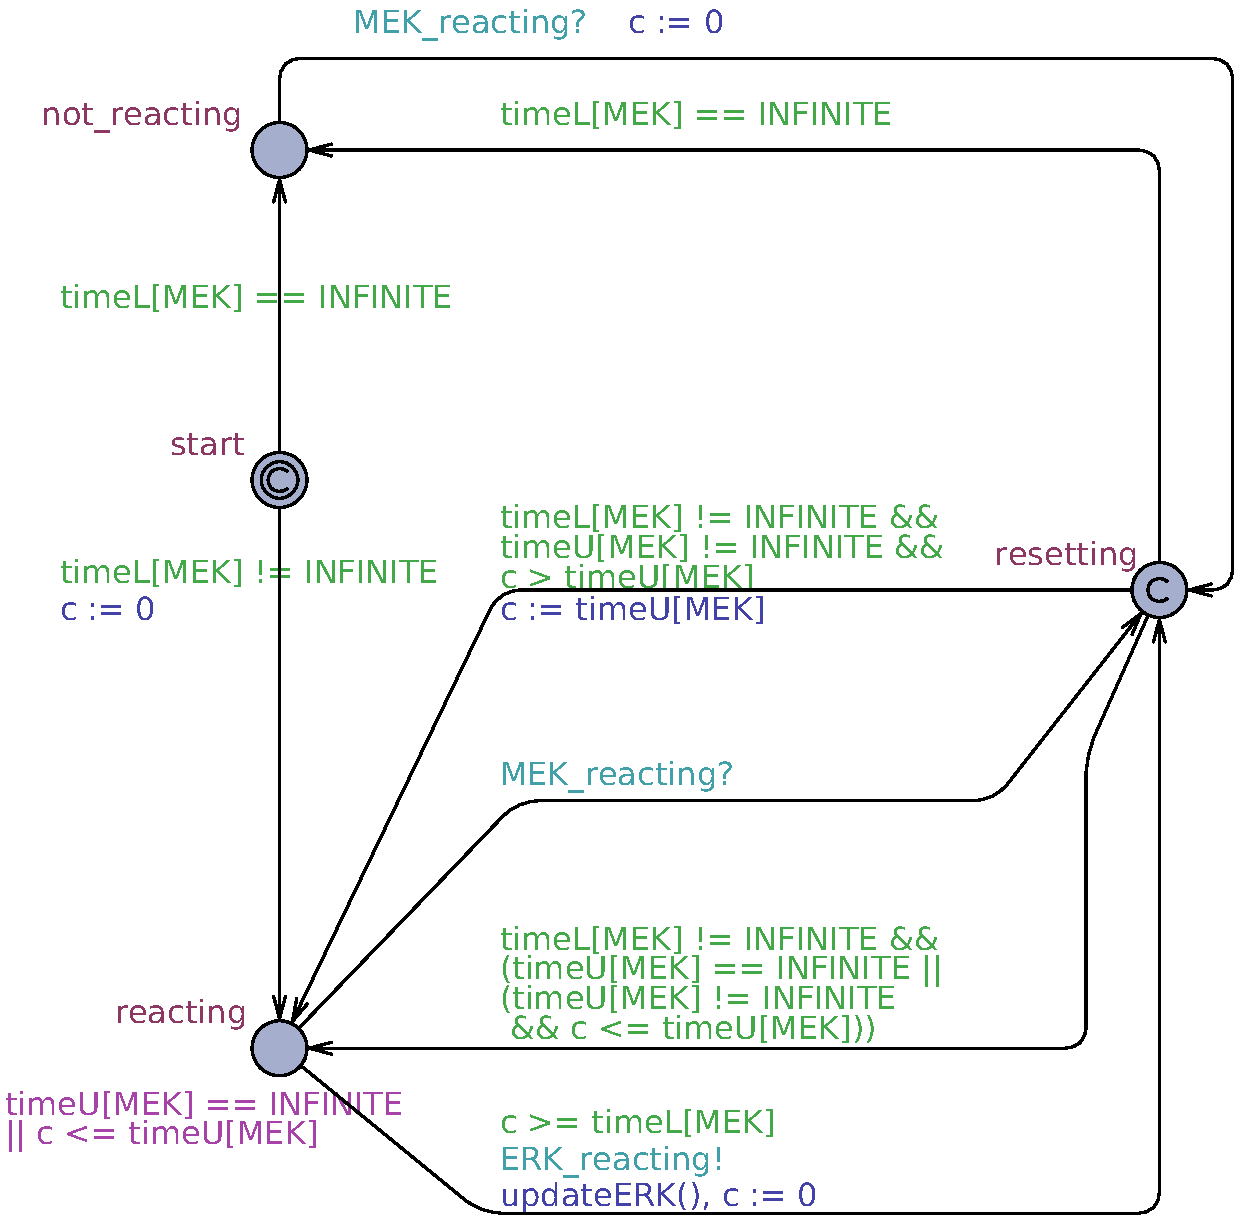
\includegraphics[width=.65\textwidth]{images/Reaction_MEK_ERK2}%ta_model_simpler}
  \caption{Timed Automaton representing a reaction where the activity level of ERK is changed with a speed depending on
the activity level of MEK. The template shown here has been simplified only to improve readability, while keeping the
same behavior as the one actually generated by ANIMO.}\label{fig:ta-model-simpler}
\end{minipage}
\end{figure}

We will call \emph{input variables} the variables representing the activity levels the reactants from which the automaton instance
depends, while the \emph{output variable} is the variable updated at each occurrence of the reaction. In the
example of Figure~\ref{fig:ta-model-simpler}, {\sf MEK} is the only input variable, and {\sf ERK} is the output variable.

The initial location, from which the evolution of the automaton begins, is marked with an additional circle and labeled
{\sf start}. Here the decision on whether the reaction can actually occur is made: if
the current values for the input variables determine a reaction rate of $0$,
the time needed for the reaction to complete is marked as {\sf INFINITE}, thus preventing the reaction to occur. If the
reaction cannot occur, the automaton switches to the location labeled {\sf not\_reacting}, otherwise it switches
to the location labeled {\sf reacting}. The {\sf C} present in a location (see locations {\sf start} and
{\sf resetting}) marks that location as \emph{committed}: when there are any automata in a committed location, the
evolution of the whole system is stalled (i.e., time is not allowed to pass) until all committed locations have been
abandoned. This ensures that no reaction occurs before all applicability conditions have been checked for all reactions in
the system, performing the necessary configuration adjustments.

When in the {\sf not\_reacting} location, the automaton is waiting for one of its input variables
to change, possibly changing the time settings for the current reaction.
As any change to reactant R is communicated through the
channel {\sf R\_reacting}, the automaton waits for changes in input variables by
waiting for a communication on their corresponding channels. Whenever such a communication is received,
the automaton switches to the {\sf resetting} location.

If the automaton is in the {\sf reacting} location, it may update its output variable when the internal reaction clock {\sf c}
is inside the allowed interval $[{\sf timeL}, {\sf timeU}]$: this means that the reaction can occur
\emph{at any moment} inside the interval.
The condition that allows the reaction to occur is described in the model by the
invariant for the {\sf reacting} location, which requires that {\sf c} must never exceed the upper bound {\sf timeU}, and by the guard
for updating the output variable, where {\sf c} is required to be greater than or equal to the lower
bound {\sf timeL}. If the reaction occurs, the output reactant is updated, signaling that the update has been performed via the
respective channel, and the automaton moves to the {\sf resetting} location. The same location is also reached if another
reaction happens that modifies the value of any input variable, because the conditions for the applicability
of the reaction at hand need to be verified again.

When in the {\sf resetting} location, the \ta\ performs a number of checks to identify the current situation, which
can be one of three possible states:
\begin{enumerate}
  \item\label{enum:cond1} the reaction can still occur
    and the clock is inside the allowed bounds (in Figure~\ref{fig:ta-model-simpler},
    this condition corresponds to guard {\sf timeL[MEK] != INFINITE \&\& (timeU[MEK] == INFINITE \textbar\textbar\ (timeU[MEK] != INFINITE \&\& c $<$= timeU[MEK]))}),
  \item\label{enum:cond2} the reaction can occur, but the changed conditions require an update to the clock in order to
    respect the invariant of location {\sf reacting} (guard {\sf timeL[MEK] != INFINITE \&\& timeU[MEK] != INFINITE \&\& c $>$ timeU[MEK]}),
  \item\label{enum:cond3} the reaction cannot occur (guard {\sf timeL[MEK] == INFINITE}).
\end{enumerate}
In case~\ref{enum:cond1}, the automaton returns to location {\sf reacting} without performing any change.
If the clock is larger than the upper time bound (case~\ref{enum:cond2}), it is updated accordingly before
moving to {\sf reacting}. Finally, if the conditions of applicability of the reaction do not hold anymore (case~\ref{enum:cond3}),
the automaton moves to location {\sf not\_reacting}, where it waits for a change in the current conditions.





\subsection{Simplified kinetic rate laws}\label{subsec:kinetic-scenarios}
Each reaction in our model is based on its two tables {\sf timeL} and {\sf timeU}. These represent
respectively the lower and upper bound for the time taken by the reaction to change its output variable by 1.
The time tables are indexed by the current value of the input variables for that reaction, and are pre-computed
based on all possible values of those inputs. Thus, if a reaction has two input variables with
5 and 13 possible activity levels respectively, the two time tables {\sf timeL} and
{\sf timeU} will contain $5 \times 13 = 65$ elements each.

In order to compute the reaction times,
ANIMO provides three different simplified kinetic rate laws that rely on a single parameter to facilitate model construction.
Since many reactions in signal transduction are enzyme-substrate reactions,
we abbreviate concentrations of upstream proteins with $E$, and of downstream proteins with $S$.
The three simplified kinetic scenarios are defined as follows.

\begin{enumerate}
  \item {\bf Scenario 1:} $r = k \times [E]$\\ Reaction rate $r$ depends only on the activity level of the upstream reactant (i.e., the one from which
the interaction arrow starts). Thus, if the upstream reactant $E$ is completely inactive, the reaction rate is zero.
Increasing the activity level of $E$ will make the reaction rate increase, thus decreasing the reaction time.
In this scenario $E$ is the only input variable of the reaction, so the time tables {\sf timeL} and {\sf timeU} are unidimensional.\\
This is the simplest scenario: in the case of a constantly active upstream reactant, the downstream reactant will be activated
with constant rate.
  \item {\bf Scenario 2:} $r = k \times [E] \times [S]$\\ $r$ depends on the activity level of two reactants, where $E$ represents the
upstream reactant and $S$ is linked to the downstream reactant (the one where the interaction arrow arrives).
If the reaction activates the downstream reactant, $S$ represents the concentration of inactive downstream reactant, thus the reaction rate increases with decreasing activity of $S$.
If the reaction inhibits the downstream reactant, $S$ represents the active fraction of the downstream reactant and the reaction rate increases with increasing activity level of $S$.
The dependence from the upstream component $E$ is the same as for Scenario 1.\\
This scenario can be used to describe activations or inhibitions that flatten off near complete activity or inactivity of $S$, respectively. % (Fig.~\ref{fig:small-model-third-graph}).
  \item {\bf Scenario 3:} $r = k \times [E_1] \times [E_2]$\\ $r$ depends on two user-chosen reactants, and influences the activity of
the reactant downstream of the reaction. The dependence from the active or inactive
fraction of $E_1$ and $E_2$ is set by the user. This scenario can be seen as the kinetic equivalent of the logical \emph{AND-gate}:
when either $E_1$ or $E_2$ is completely inactive, the reaction rate is zero.\\
As an example of application of Scenario 3, see the relation between {\sf c-Jun}, {\sf c-Fos} and {\sf AP-1} in the model of Figure~\ref{fig:large-model-complete}:
both {\sf c-Jun} and {\sf c-Fos} need to be active in order to activate {\sf AP-1}. This information is inserted in the kinetics associated to the edge
{\sf c-Jun} $\rightarrow$ {\sf AP-1}, setting $E_1 = ${\sf c-Jun} and $E_2 = ${\sf c-Fos}. The edge {\sf c-Fos} $\rightarrow$ {\sf AP-1} has a kinetic
constant $k = 0$ and is used as a reminder that also {\sf c-Fos} takes part to the reaction.
\end{enumerate}


\subsection{Translation of kinetic rate laws to time constants}\label{subsec:kinetics}

The time (in seconds) needed for a particular reaction step to complete is
computed by the formula
$$
t = \frac{1}{r} \times \mbox{\sf granularityScale} \times \mbox{\sf timeScale}.
$$
If $r = 0$, then the time is defined to be infinite (cf. the {\sf INFINITE} in Figure~\ref{fig:ta-model-simpler}),
meaning that the reaction cannot take place.
The scale factor {\sf granularityScale} is used to ensure that the values used to compute the
reaction rate $r$ are independent from the granularity (number of activity levels)
of each reactant.
Factor {\sf timeScale} (measured in $\frac{\mbox{\scriptsize TA time units}}{s}$)
is applied in order to translate seconds into \tas\ time units.
Hence, the time constants present in the time tables are given in $\frac{\mbox{\scriptsize TA time
units}}{\mbox{\scriptsize activity level}}$. Intuitively, each entry in the time tables can be thought of as
the answer to the question ``How many \tas\ time units are needed to increase/decrease the output variable
of this reaction with the current value of the input variables?''.

Finally,
we generalize time constants to time intervals, introducing a $5\%$ variability:
the exact duration $t$ of a reaction computed via the kinetic formula becomes the interval $[0.95\times t, 1.05\times t]$.
The two extremes of the interval are saved each in its own table, thus obtaining a lower bound and an upper bound table,
both indexed by the current activity levels of the input variables of the reaction at hand.
The two time bounds correspond to the ones identified by the constants $18$ and $20$ in Figure~\ref{subfig:mek}.
The tables where those bounds are stored are called $R_{\mbox{\scriptsize lowerBound}}$ and $R_{\mbox{\scriptsize upperBound}}$
in Figure~\ref{fig:ta-diagram} and {\sf timeL}, {\sf timeU} in Figure~\ref{fig:ta-model-simpler}.



\subsection{Different choices for the number of levels of a node}
Figure~\ref{fig:levels} shows the differences between different choices for the
number of levels of a node. This allows to adapt a model to the quality of experimental data.

\begin{figure}[htpb]
\begin{minipage}{\textwidth}
\centering
\subfloat[\label{suppl:fig1-1level}]{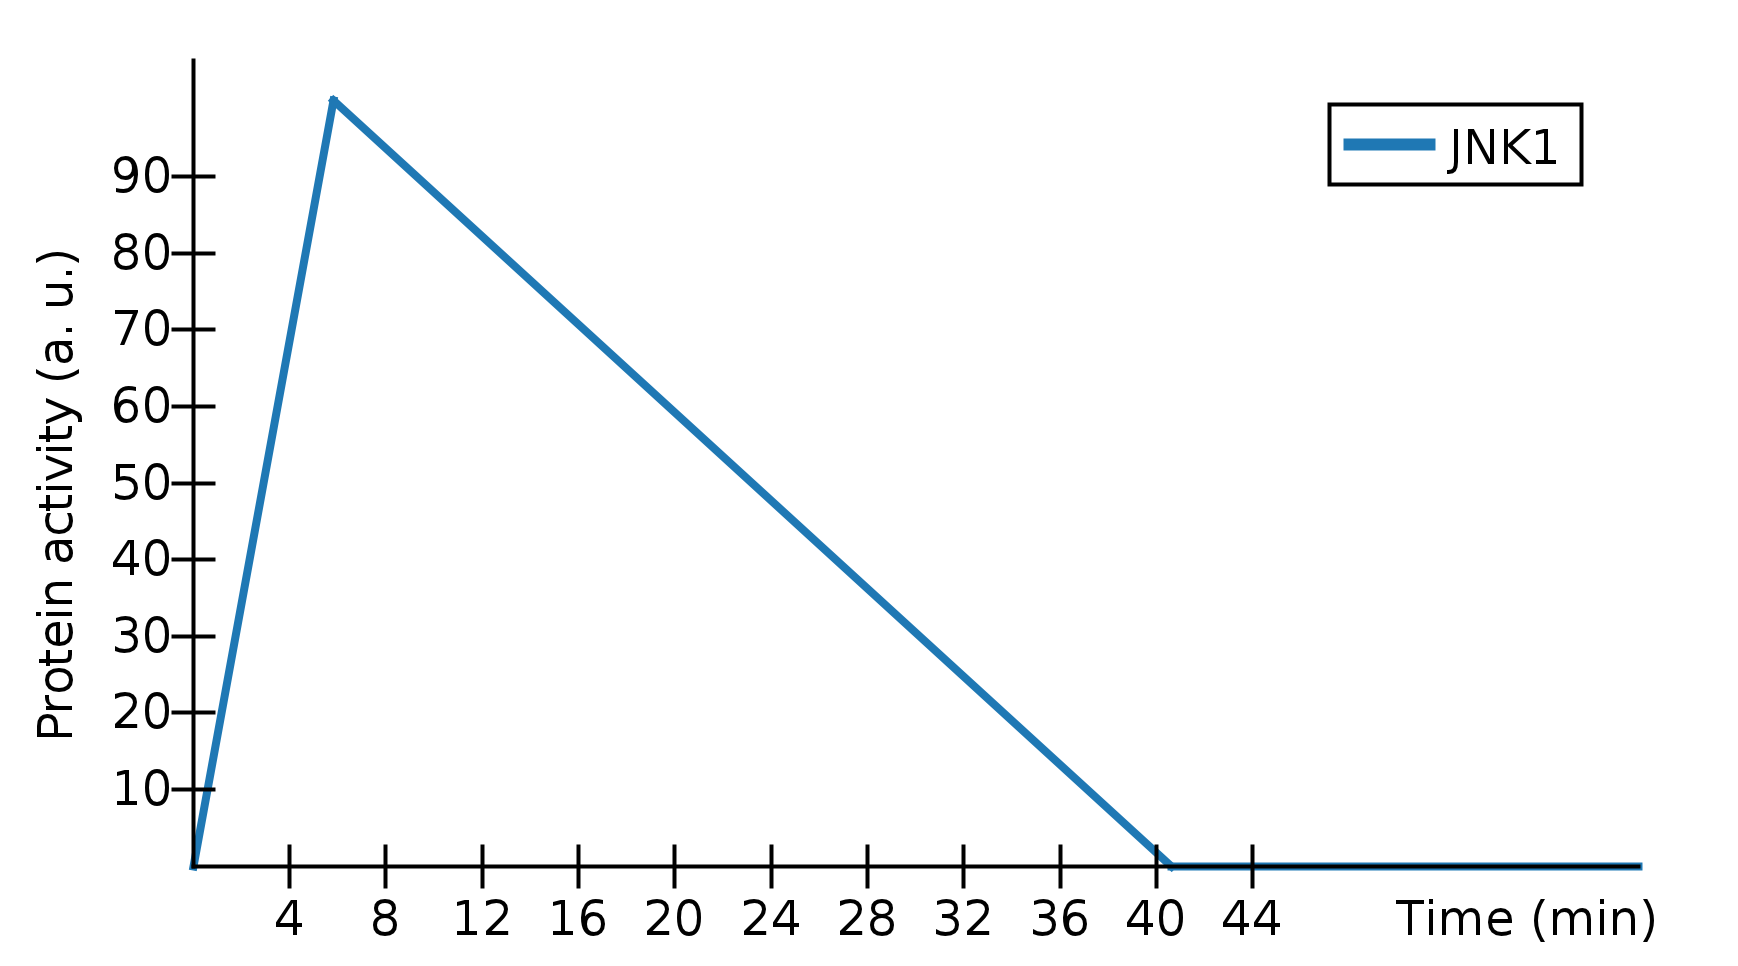
\includegraphics[width=.45\textwidth]{images/JNK1_1level2}} \qquad
\subfloat[\label{suppl:fig1-10levels}]{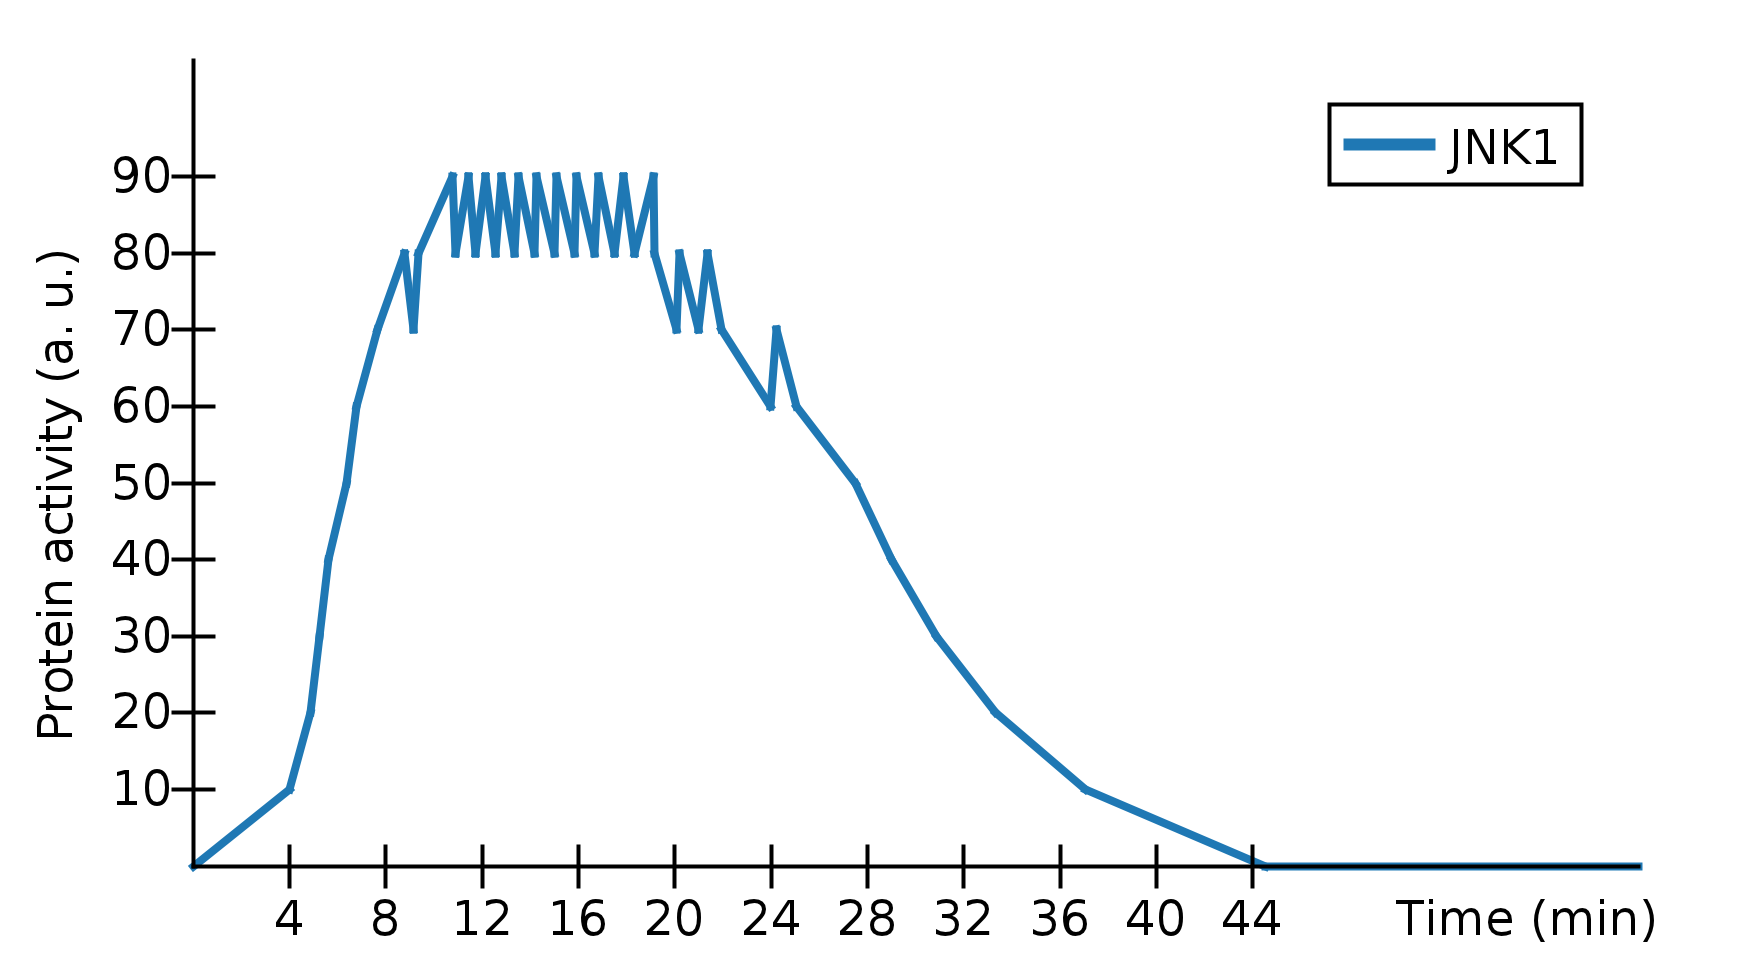
\includegraphics[width=.45\textwidth]{images/JNK1_10levels2}} \\
\subfloat[\label{suppl:fig1-50levels}]{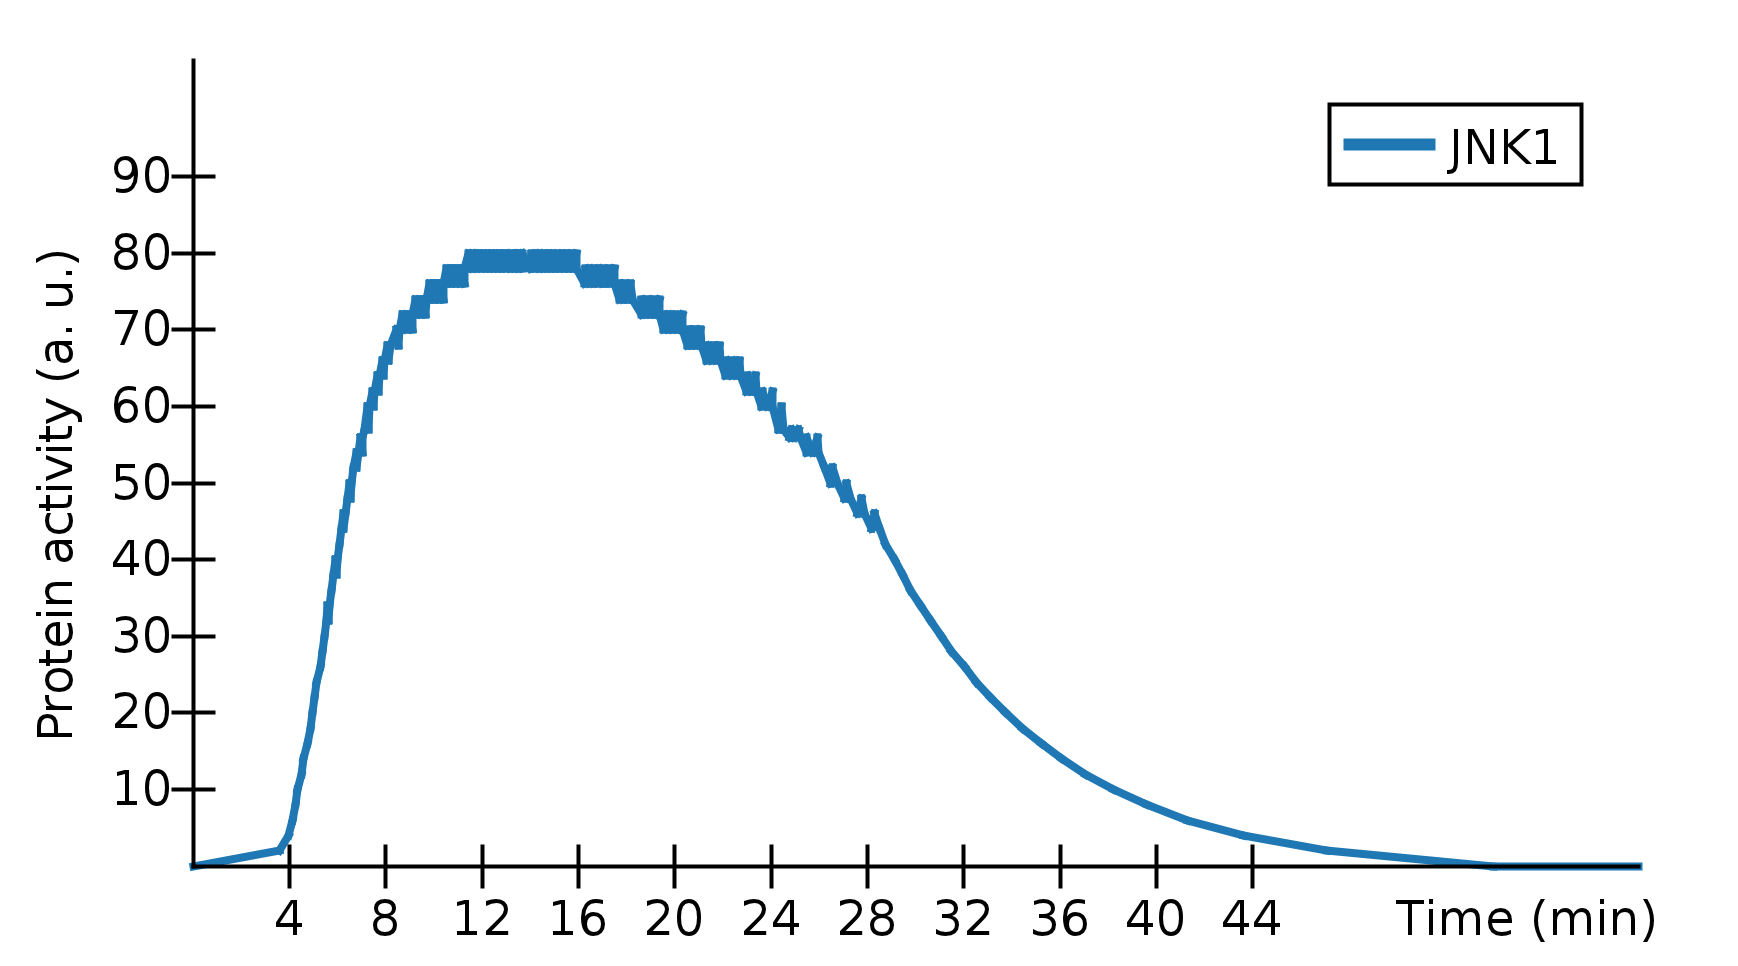
\includegraphics[width=.45\textwidth]{images/JNK1_50levels2}} \qquad
\subfloat[\label{suppl:fig1-100levels}]{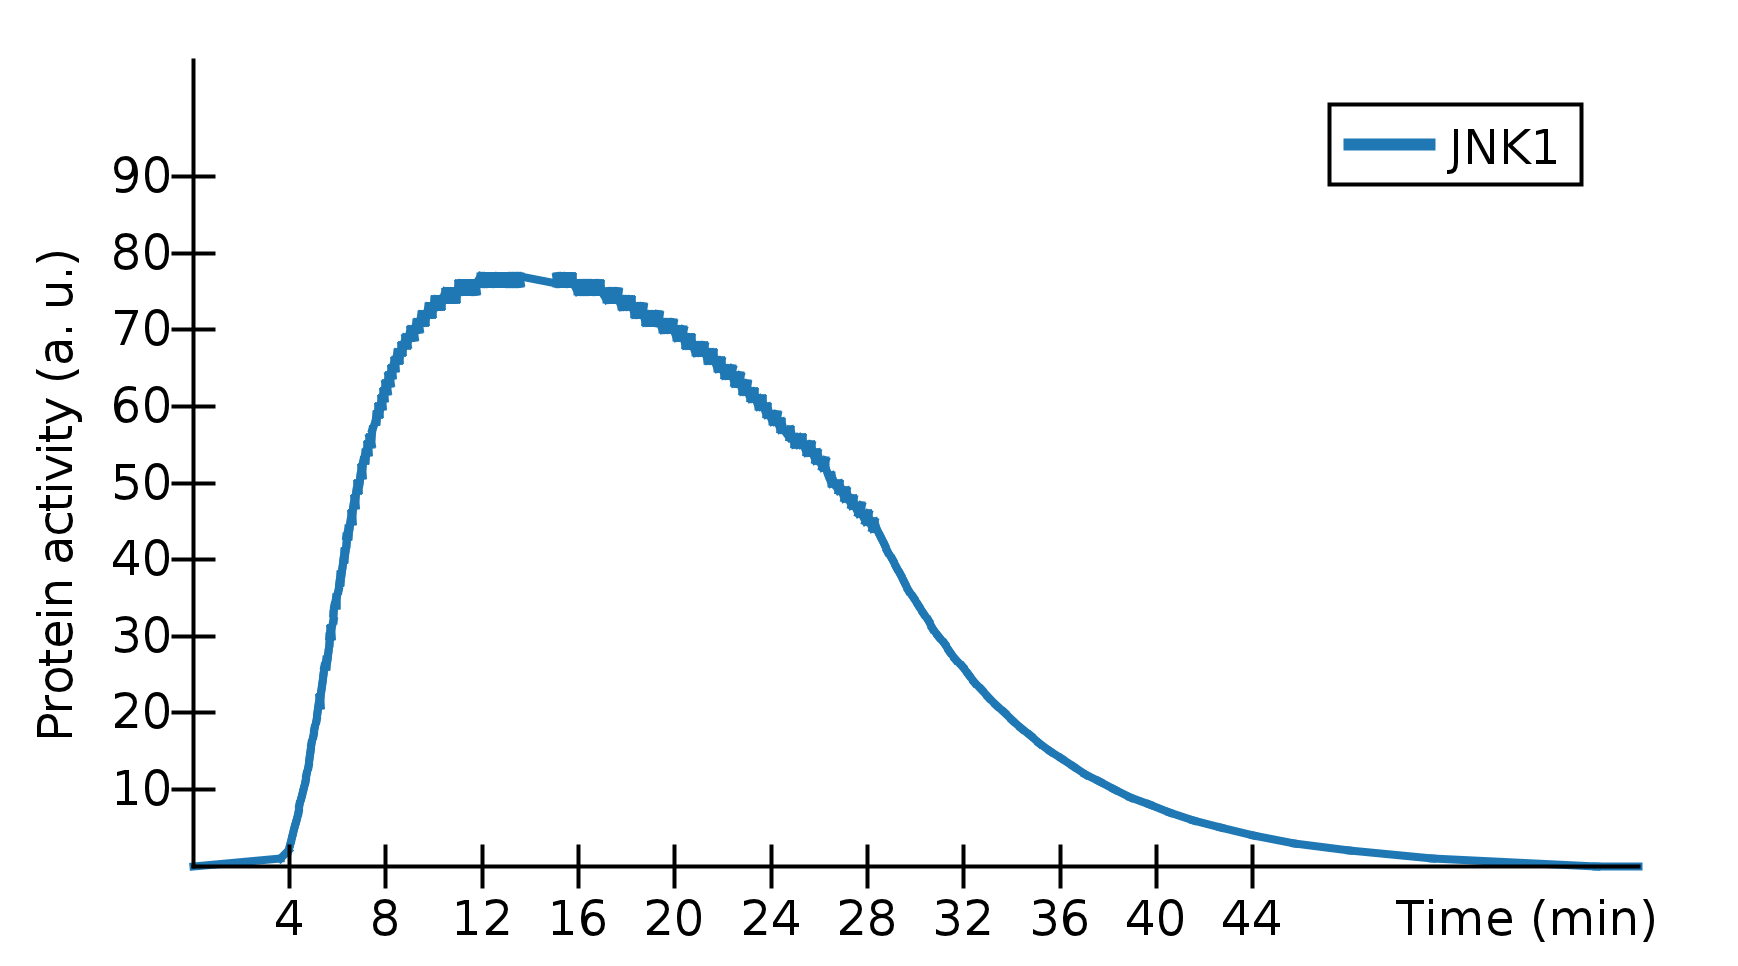
\includegraphics[width=.45\textwidth]{images/JNK1_100levels2}}
\caption{Comparing different reactant granularity settings. {\bfseries (\protect\subref*{suppl:fig1-1level})} 2 levels, {\bfseries (\protect\subref*{suppl:fig1-10levels})} 10 levels,  {\bfseries (\protect\subref*{suppl:fig1-50levels})} 50 levels, {\bfseries (\protect\subref*{suppl:fig1-100levels})} 100 levels. The {\sf JNK1} series is computed from the model presented in Figure~\ref{fig:large-model-complete}, considering 100 ng/ml TNF$\alpha$ as treatment condition over a period of 60 minutes.}\label{fig:levels}
\end{minipage}
\end{figure}



\section{Comparison between ANIMO and other modeling tools}\label{suppl:comparison-table}
Different formalisms are in use in the field of computational
modeling of biological systems, each with their specific characteristics.
Many of these formalisms have been implemented into
software tools to support modelling efforts. In order to compare
ANIMO with existing tools, we have selected a number of mathematical formalisms,
each connected to a supporting tool. With an emphasis on the modeling
process rather than the final model, we compared these tools on
the basis of the following parameters:

\begin{enumerate}
  \item {\bf Hidden formalism:} a knowledge of the underlying formalism is not required in order to use the tool
  \item {\bf Visual modeling:} the tool allows the user to model using a visual interface, and is not exclusively
      founded on formula-, text- or table-based input forms
  \item {\bf Qualitative parameters:} parameters for reactions can be input as approximated estimations, and not exclusively as numbers
  \item {\bf Tight coupling with topology:} models are tightly and clearly coupled to the networks they represent, showing the visual
      representation of the model in a shape similar or comparable to the representation currently used by biologists
      for signaling pathways
  \item {\bf User-chosen granularity:} if discretization is applied during the modeling process, the user can change the granularity
      with which such discretization is made, possibly for each component of the model separately
\end{enumerate}
Table~\ref{tab:tool-comparison} shows the comparison between ANIMO and the selected tools.

\newcolumntype{x}[1]{%
>{\centering\hspace{0pt}}p{#1}}%
\savenotes
\begin{table}[!hbt]
\begin{minipage}{\textwidth}
\processtable{Comparison between ANIMO and some existing approaches to modeling biological systems.
A ``Yes'' under a column indicates that the modeling tool (mostly) fulfills the parameter, ``No'' indicates very limited or no fulfillment.
\label{tab:tool-comparison}}
{\begin{tabular}{p{4cm}p{1.8cm}p{1.8cm}p{1.5cm}p{1.8cm}p{1.8cm}p{2cm}}
\toprule
{\bfseries Tool} & {\bfseries Formalism} & {\bfseries Hidden formalism} & {\bfseries Visual modeling} & {\bfseries Qualitative parameters} & {\bfseries Tight coupling with topology} & {\bfseries User-chosen granularity}  \\[5mm]
\midrule
\noalign{\vskip 2mm} ANIMO~\citep{animo-bibe} & Timed \ \ \ Automata & Yes & Yes & Yes & Yes & Yes
      \\[5mm]
\noalign{\vskip 2mm} Bio-PEPA Workbench~\citep{biopepa-interface} & Bio-PEPA & No & No & No & No & Yes
      \\[5mm]
\noalign{\vskip 2mm} Cell Illustrator~\citep{cell-illustrator} & Petri Nets & Yes & Yes & No & Yes & No
     \\[5mm]
\noalign{\vskip 2mm} COPASI~\citep{copasi} & ODE, stochastic models & No & No & No & No & No
      \\[5mm]
\noalign{\vskip 2mm} COSBI LAB~$^1$
 & BlenX & Yes & Yes & No & Yes & No
      \\[5mm]
\noalign{\vskip 2mm} GINsim~\citep{ginsim} & Boolean Networks & No & Yes & Yes & Yes & Yes~$^2$
      \\[5mm]
\noalign{\vskip 2mm} GNA~\citep{gna}    & ODE & No & Yes & Yes & Yes & No~$^3$
      \\
\noalign{\vskip 2mm} Rhapsody~$^4$
 & Statecharts & No & Yes & Yes & No~$^5$ & No
      \\[5mm]
\botrule
\end{tabular}}{$^1$ {COSBILab} web page \url{http://www.cosbi.eu/index.php/research/cosbi-lab}\\
$^2$ The user can choose the number of levels for each reactant, allowing to define
multi-level models based on Boolean reaction dynamics.\\
$^3$ When discretizing an ODE model, the granularity depends on the mathematical
features of the model, and not directly on the user's choice.\\
$^4$ {IBM Rational Rhapsody} web page \url{http://www-01.ibm.com/software/rational/products/rhapsody/designer}\\
$^5$ Statecharts represent more closely the so-called
\emph{transition system} of the model as opposed to the components and interactions occurring among them.}
\end{minipage}
\end{table}



% \addcontentsline{toc}{section}{References}
% \begin{thebibliography}{}
% ...
% \end{thebibliography}




\clearpage

\section{Supplementary figures}\label{sec:supplementary-figures}


\begin{figure}[htpb]
\begin{minipage}{\textwidth}
\centering
  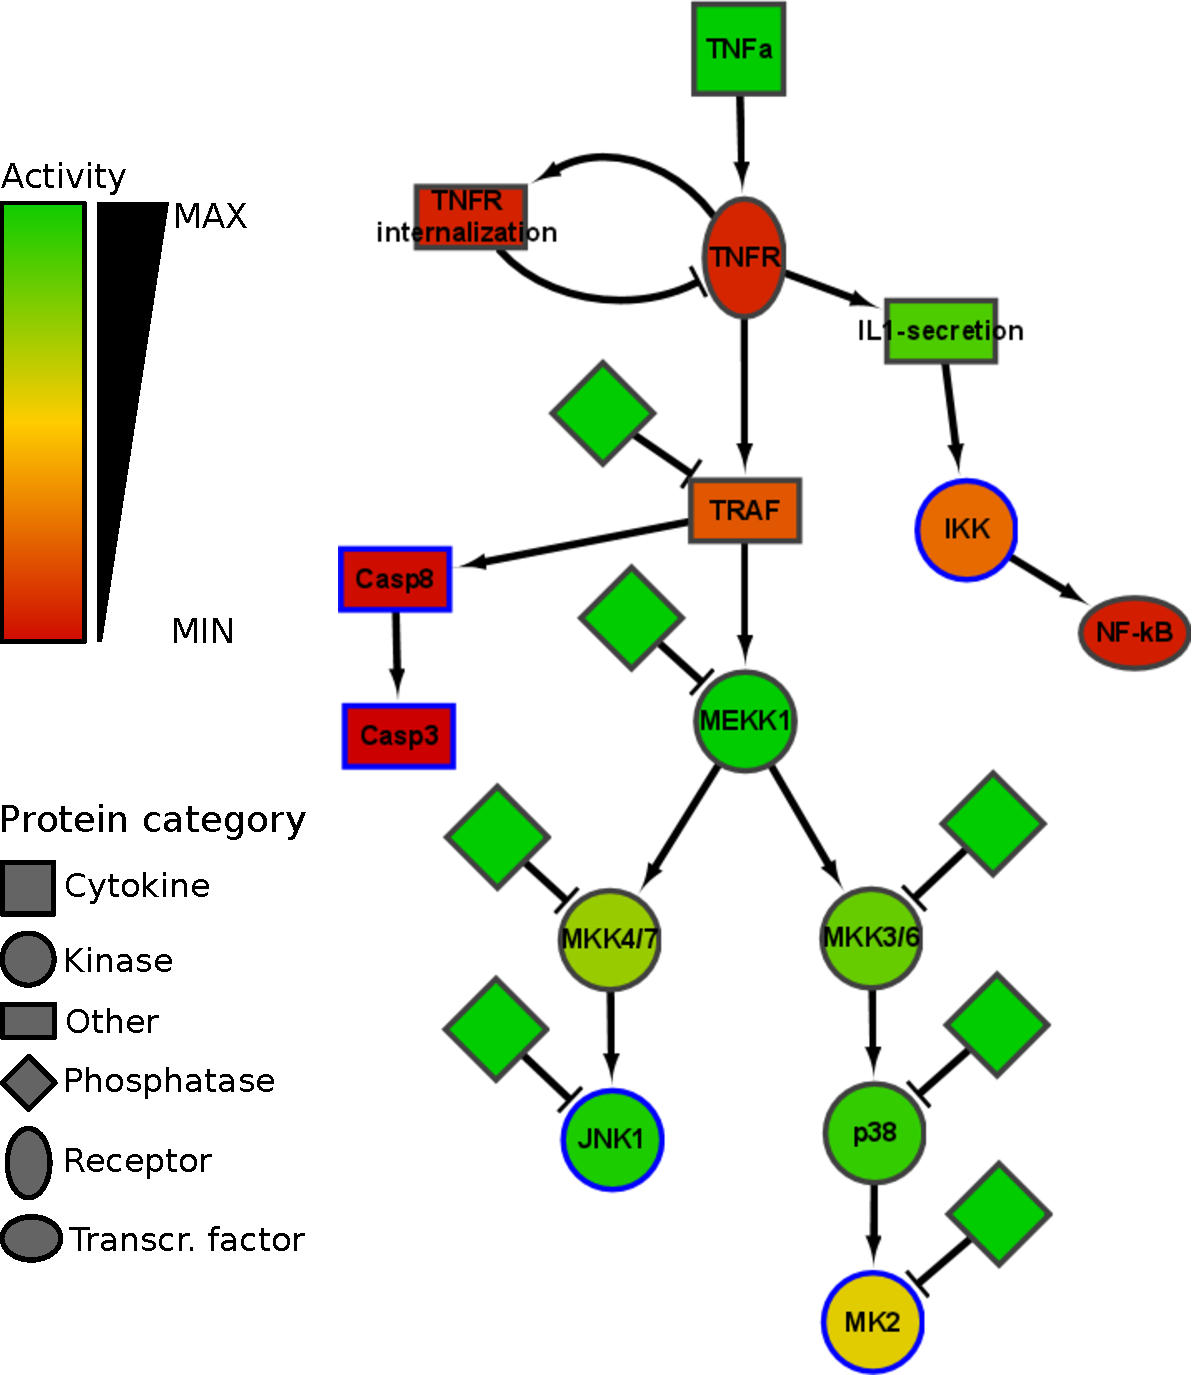
\includegraphics[width=.7\textwidth]{images/large_network_tnfa2}
\caption{The model for the TNF$\alpha$ pathway in isolation. Node colors represent the activity level of the
corresponding modeled reactants at time $t = 10$ minutes after a stimulation of 100 ng/ml TNF$\alpha$.}\label{fig:large-model-tnf}
\end{minipage}
\end{figure}

\begin{figure}[!tpb]
\begin{minipage}{\textwidth}
\centering
  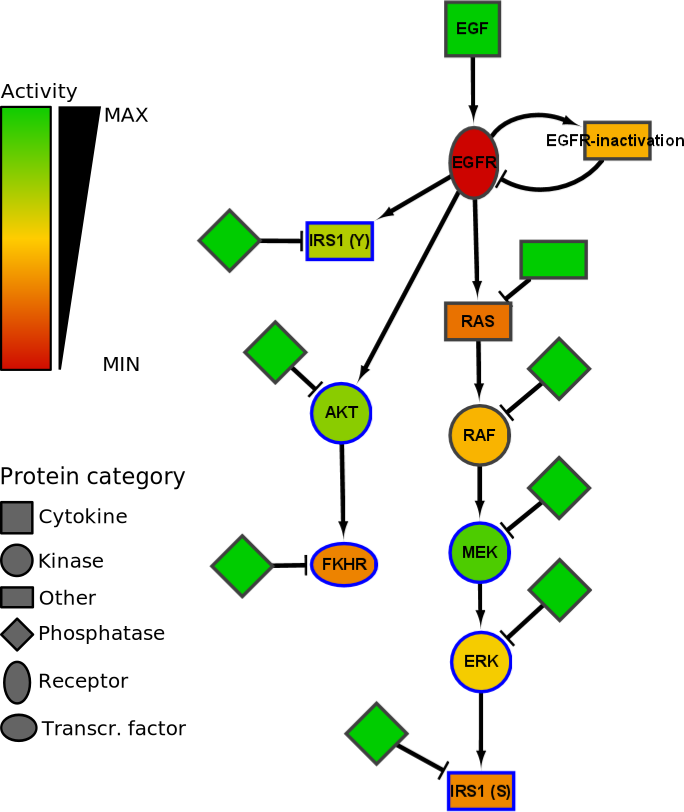
\includegraphics[width=.7\textwidth]{images/large_network_egf3}
\caption{The model for the EGF pathway in isolation. Node colors represent the
activity level of the corresponding modeled reactants at time $t = 5$ minutes after
a stimulation of 100 ng/ml EGF.}\label{fig:large-model-egf}
\end{minipage}
\end{figure}


\begin{figure}[!tpb]
\begin{minipage}{\textwidth}
\centering
  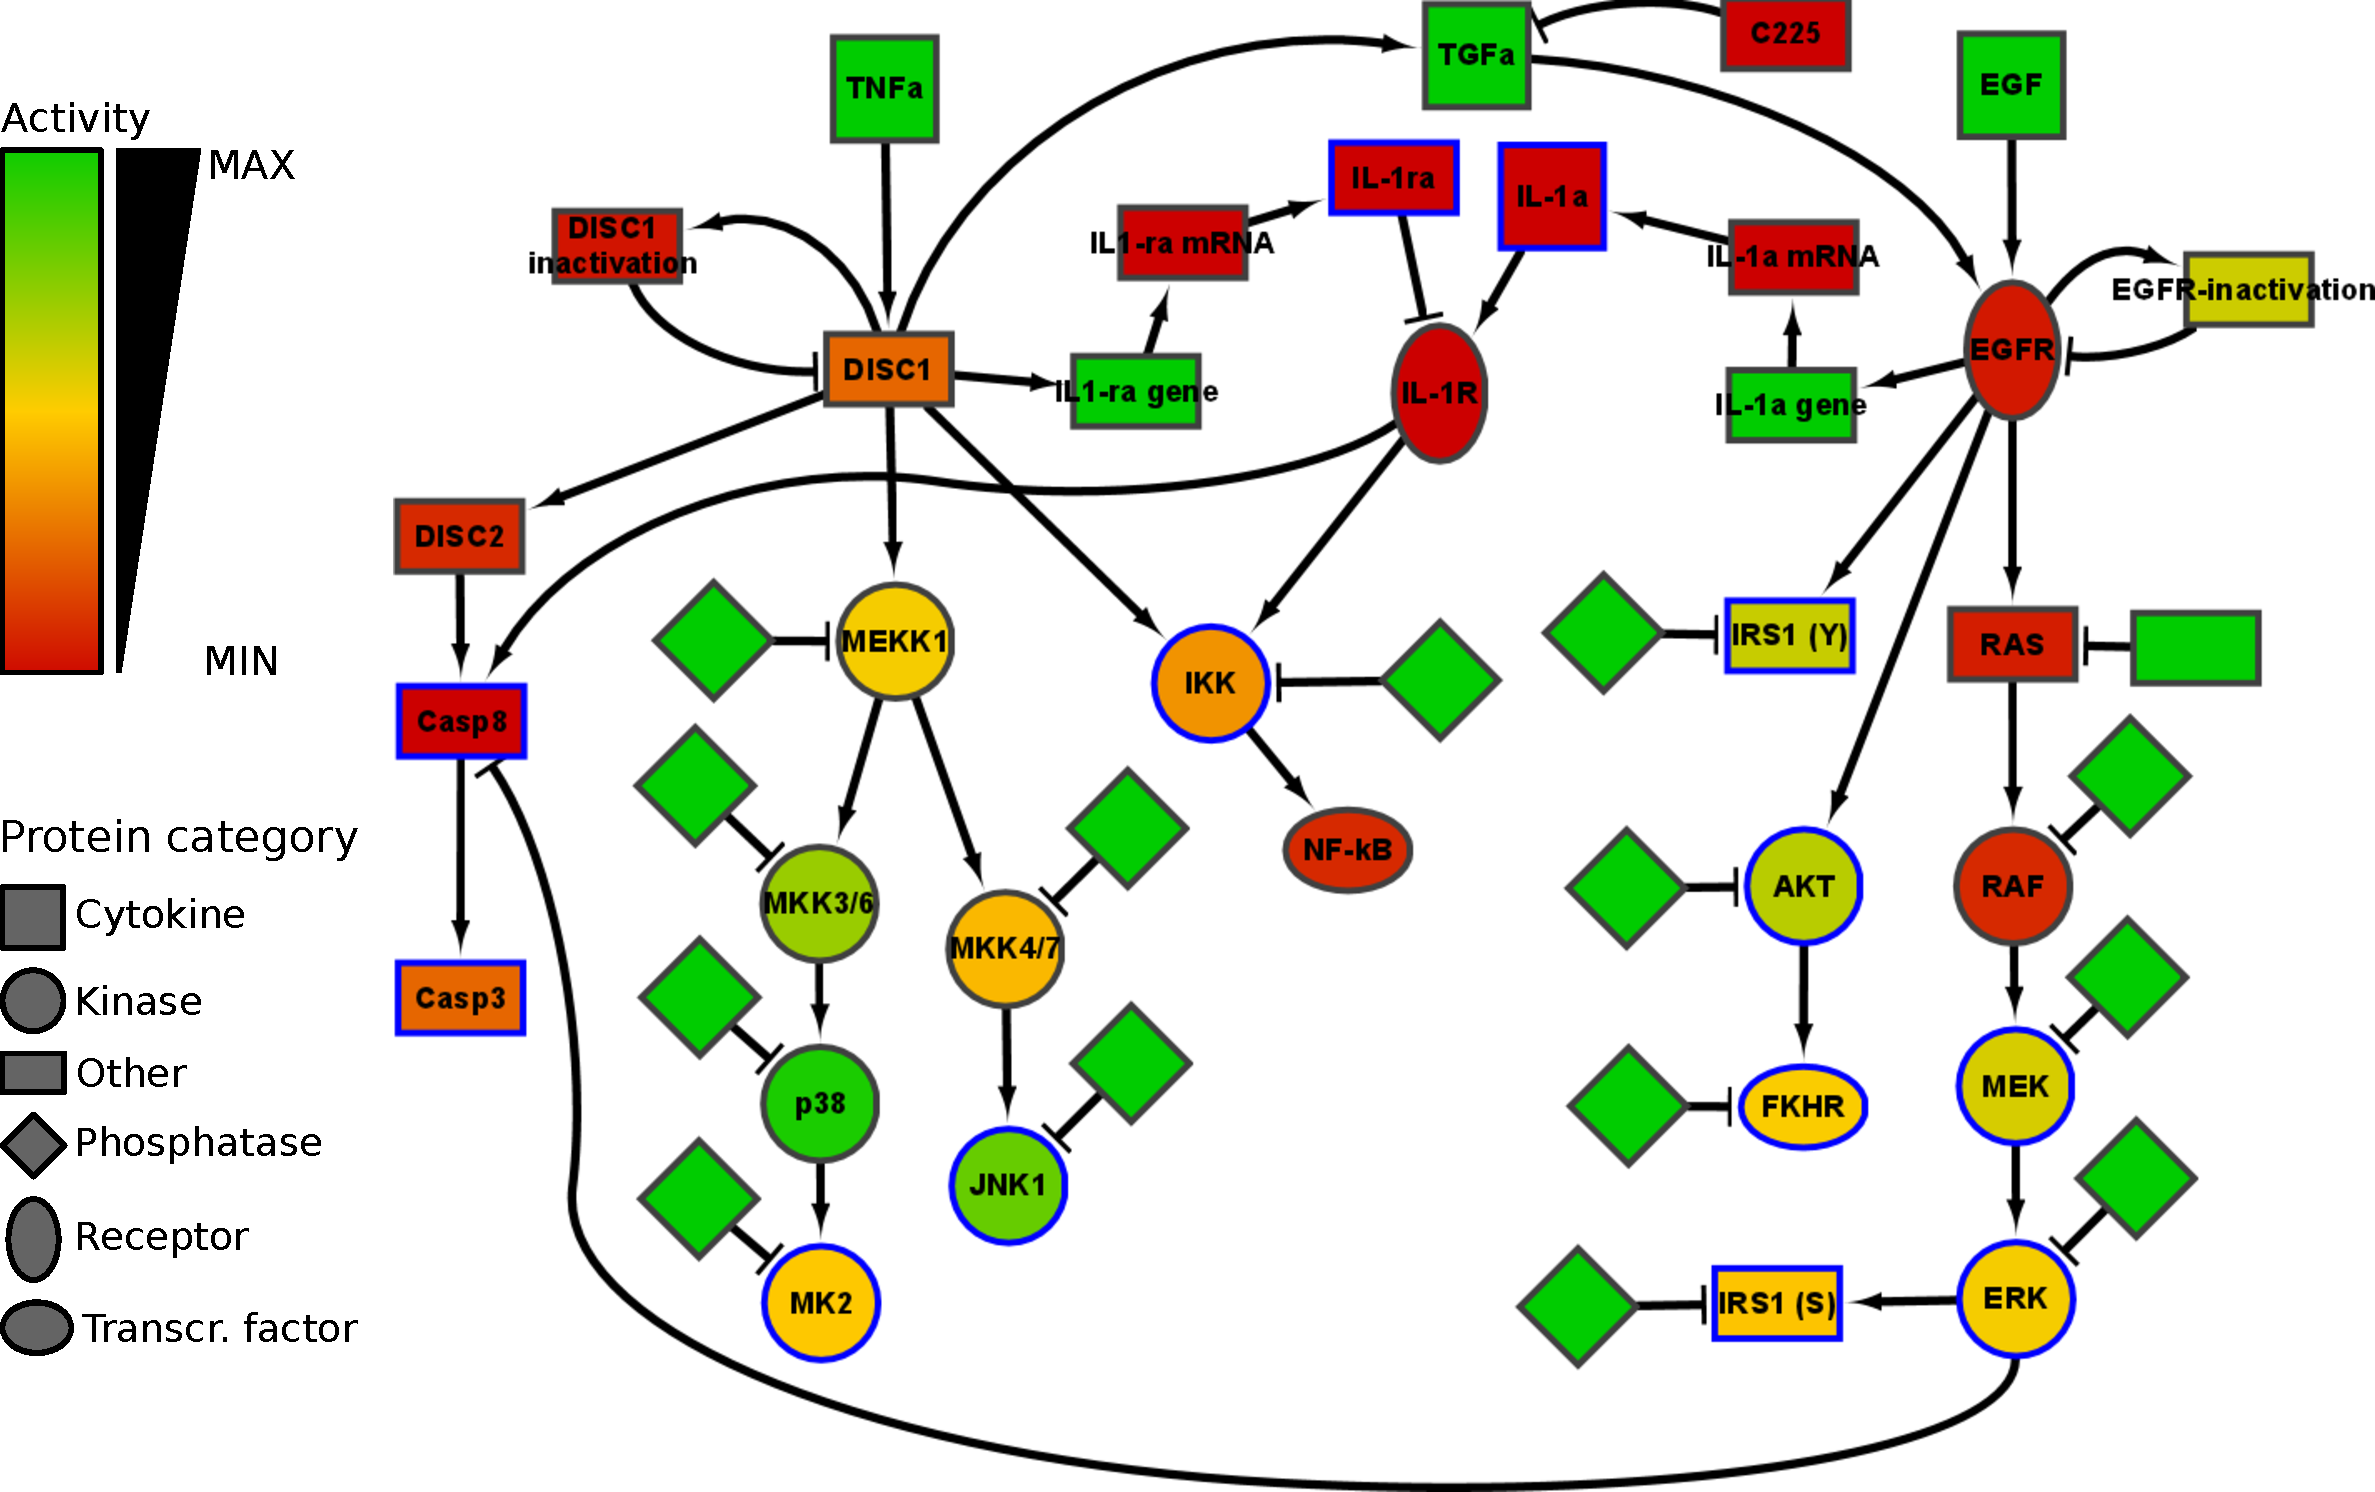
\includegraphics[width=\textwidth]{images/large_network_tnf_egf_merged_no_hyp_bis2}
\caption{The model for the merged TNF$\alpha$ and EGF pathways before
adding the hypotheses in Figure~\ref{fig:large-model-hypotheses}. Node colors represent the
activity level of the corresponding modeled reactants at time $t = 15$ minutes after
a stimulation of 100 ng/ml TNF$\alpha$ + 100 ng/ml EGF.}\label{fig:large-model-tnf-egf-merged}
\end{minipage}
\end{figure}


\renewcommand*\thesubfigure{}
\begin{figure}[!tpb]
\begin{minipage}{\textwidth}
\begin{tabularx}{\textwidth}{XXX}
\subfloat[MK2 (2 hours)]{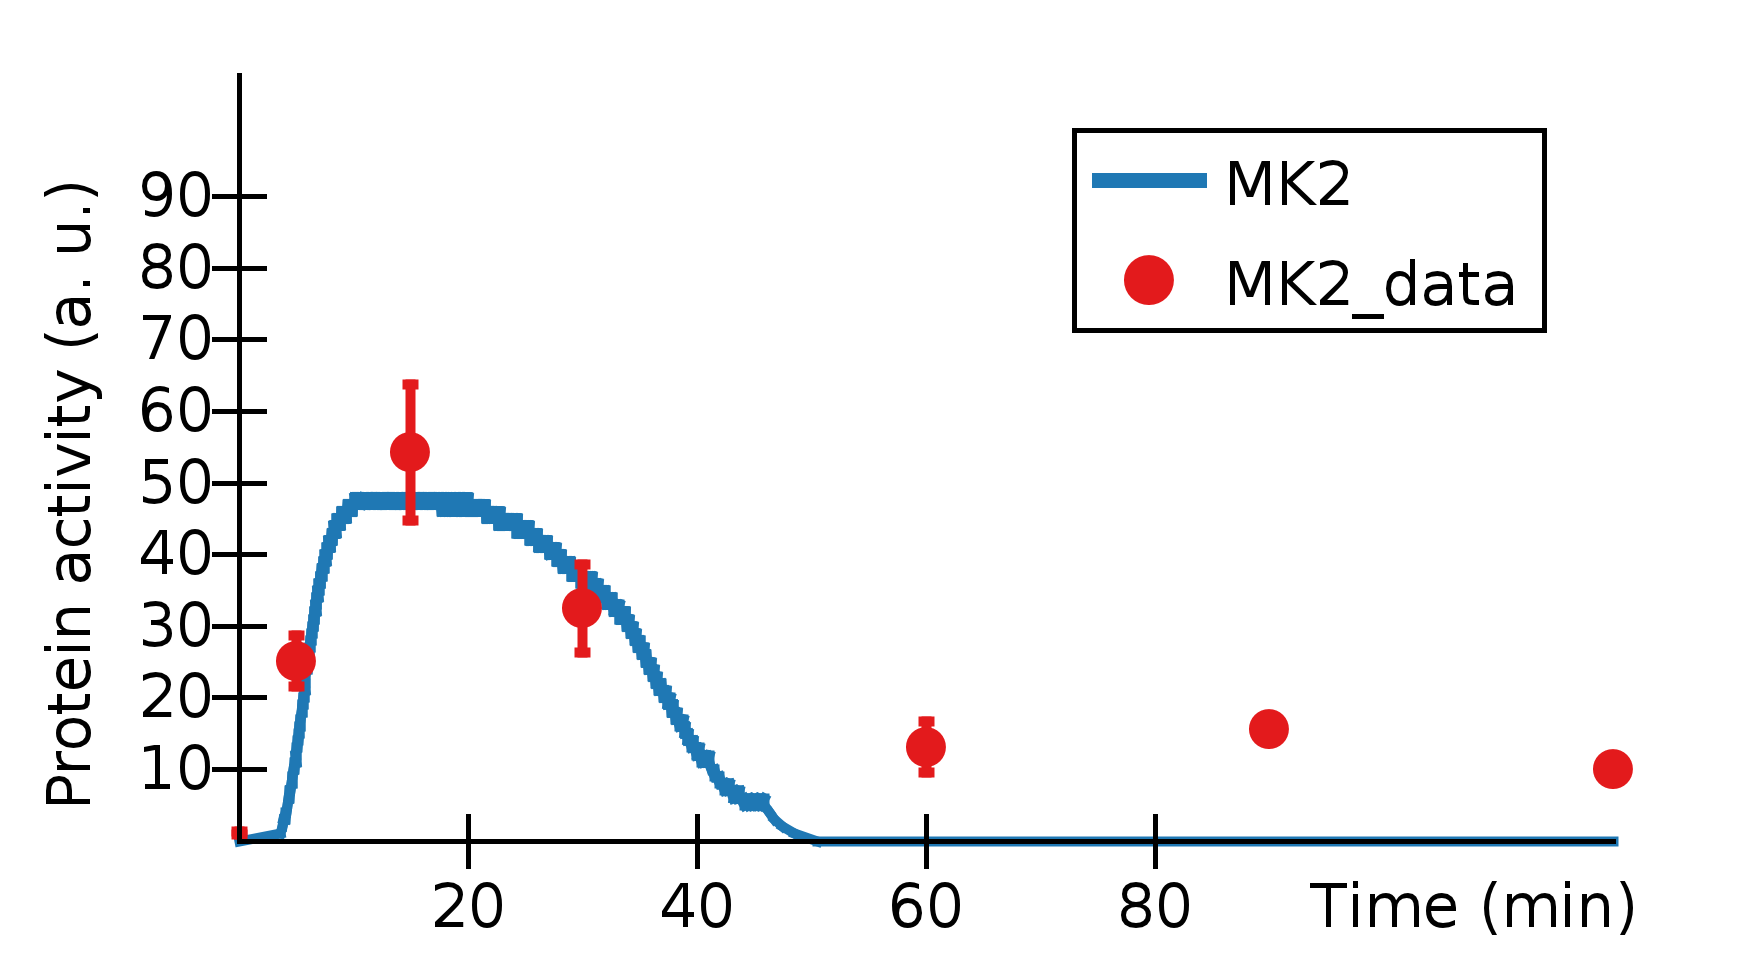
\includegraphics[width=0.29\textwidth]{images/TNFa100/MK2}} &
\subfloat[JNK1 (2 hours)]{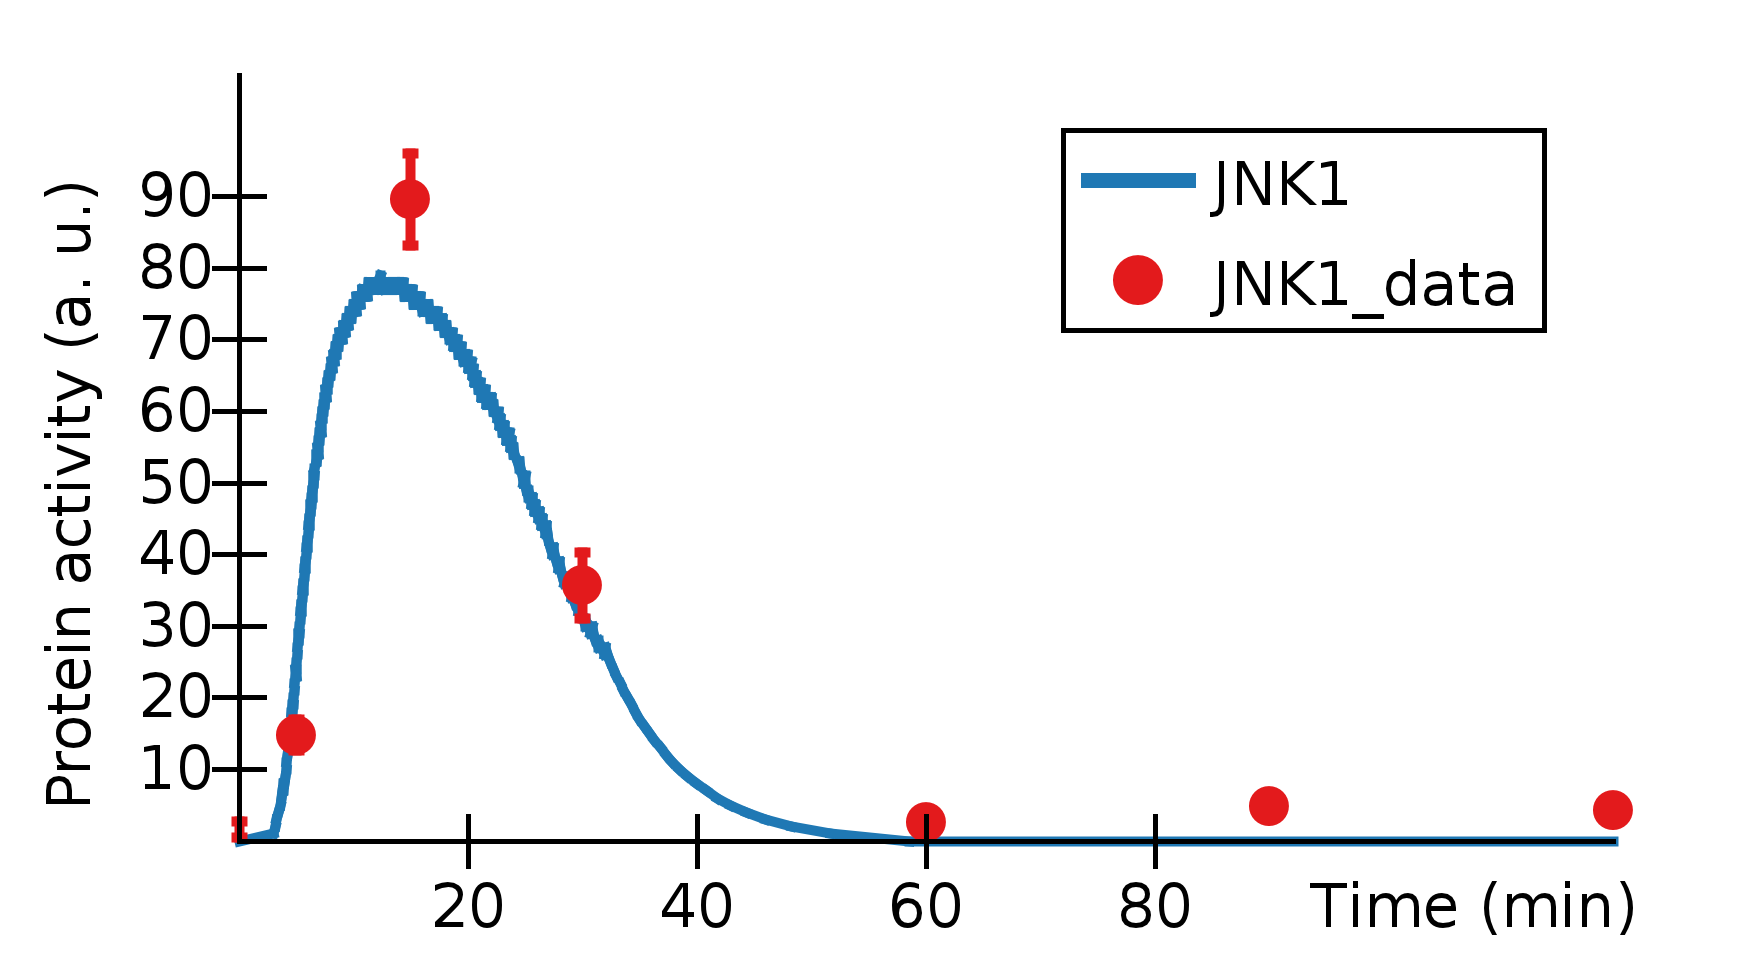
\includegraphics[width=0.29\textwidth]{images/TNFa100/JNK1}} &
\subfloat[IKK (2 hours)]{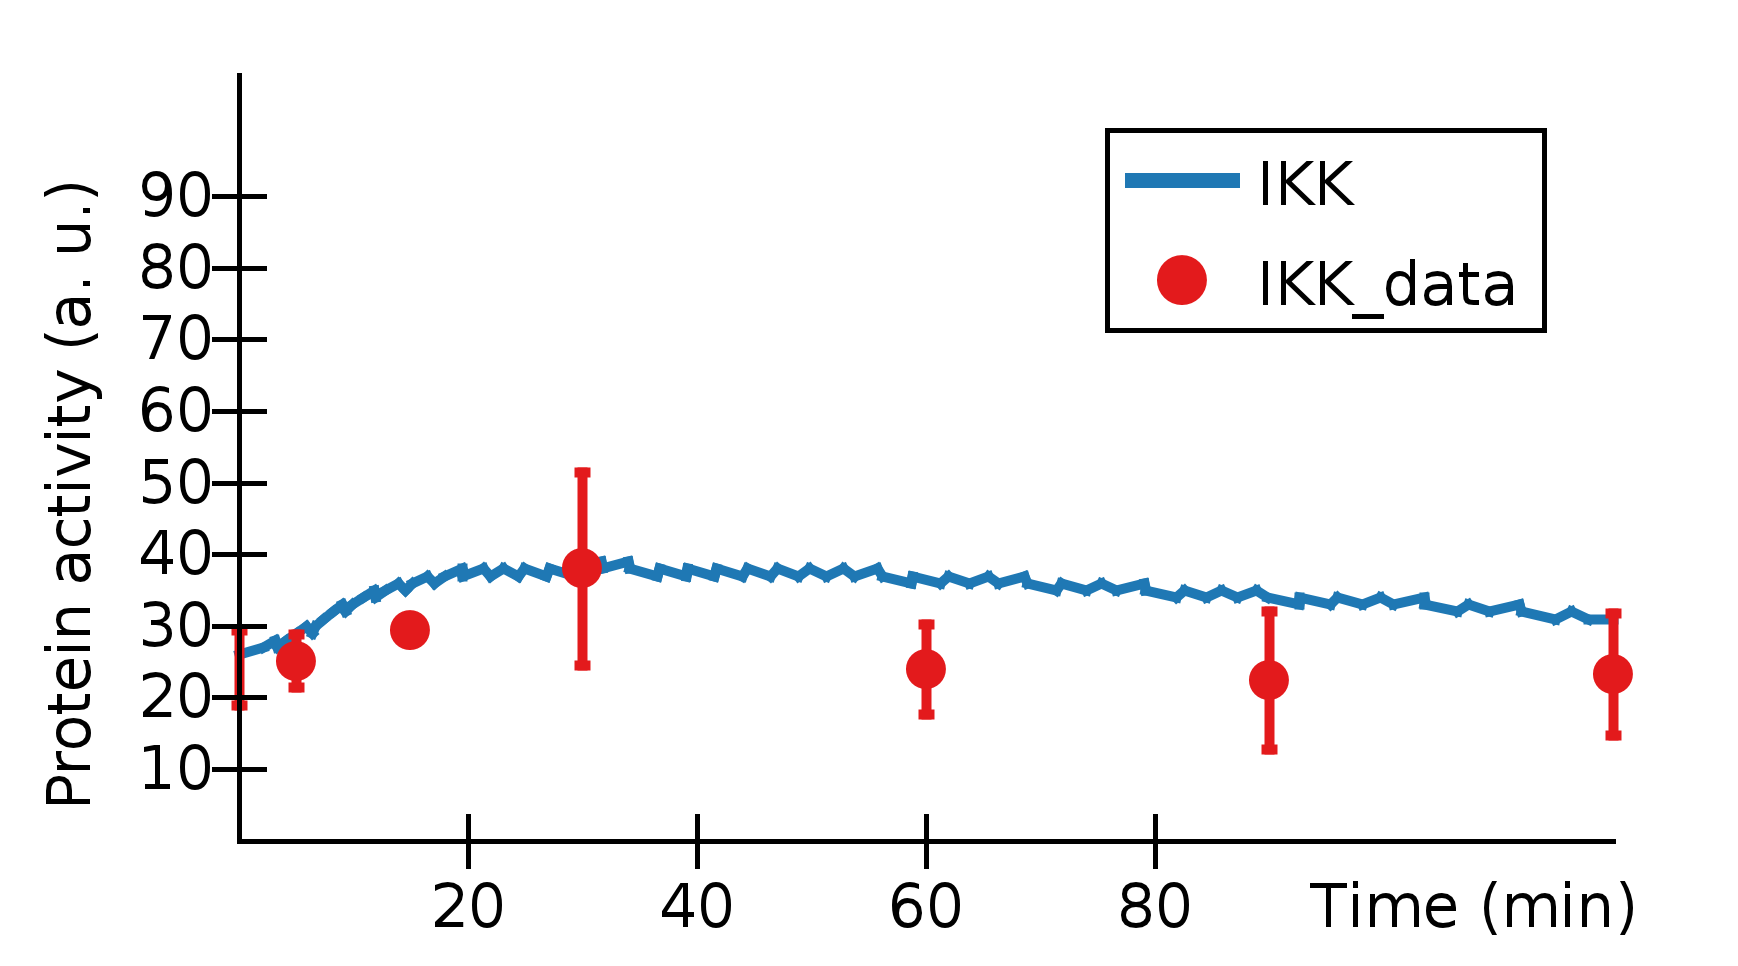
\includegraphics[width=0.29\textwidth]{images/TNFa100/IKK_120}} \\
\subfloat[IKK]{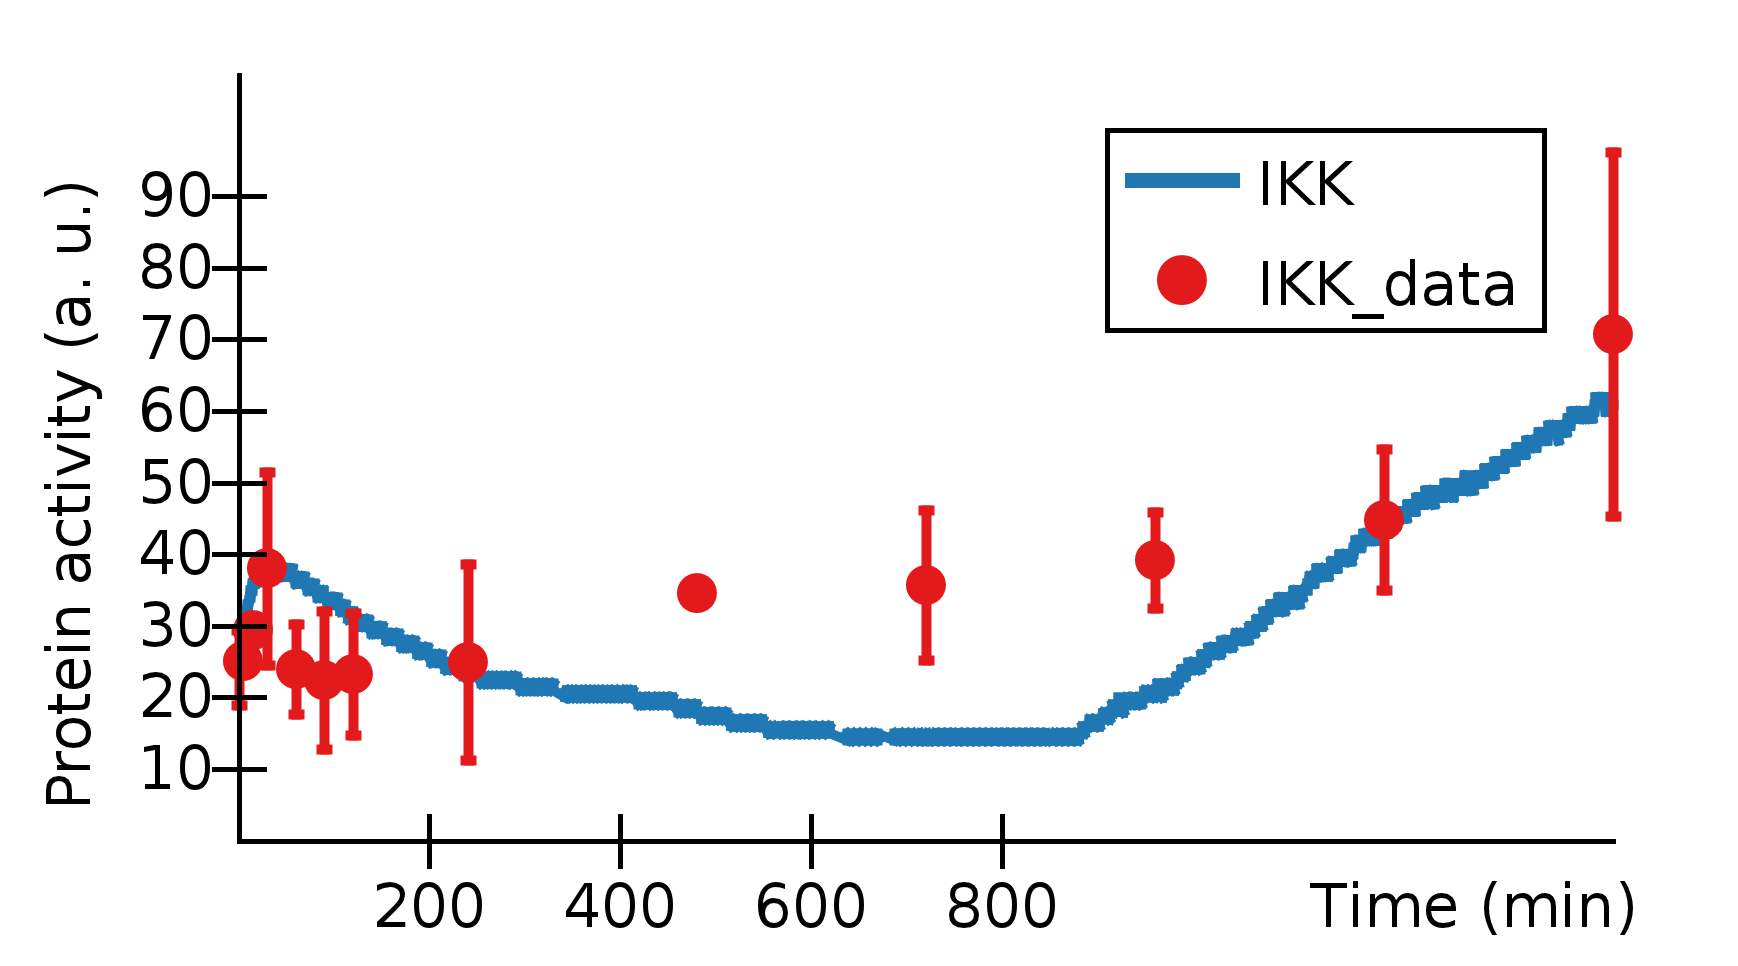
\includegraphics[width=0.29\textwidth]{images/TNFa100/IKK_1440}} &
\subfloat[caspase-8]{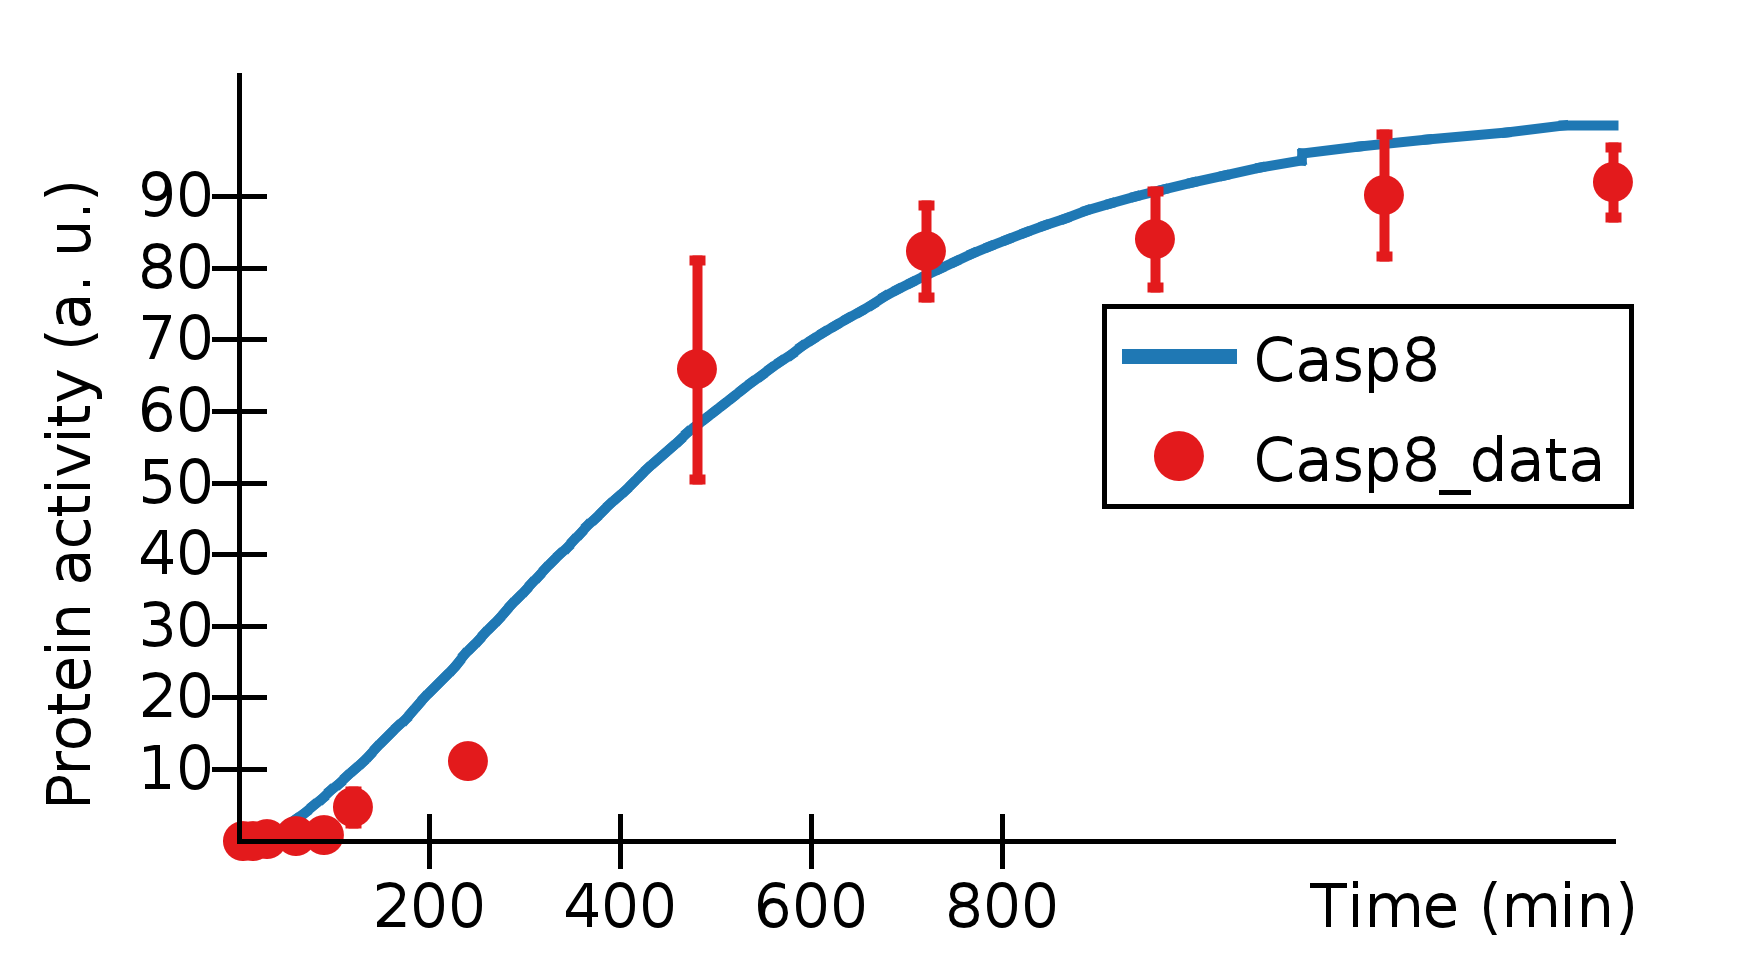
\includegraphics[width=0.29\textwidth]{images/TNFa100/casp8}} &
\subfloat[caspase-3]{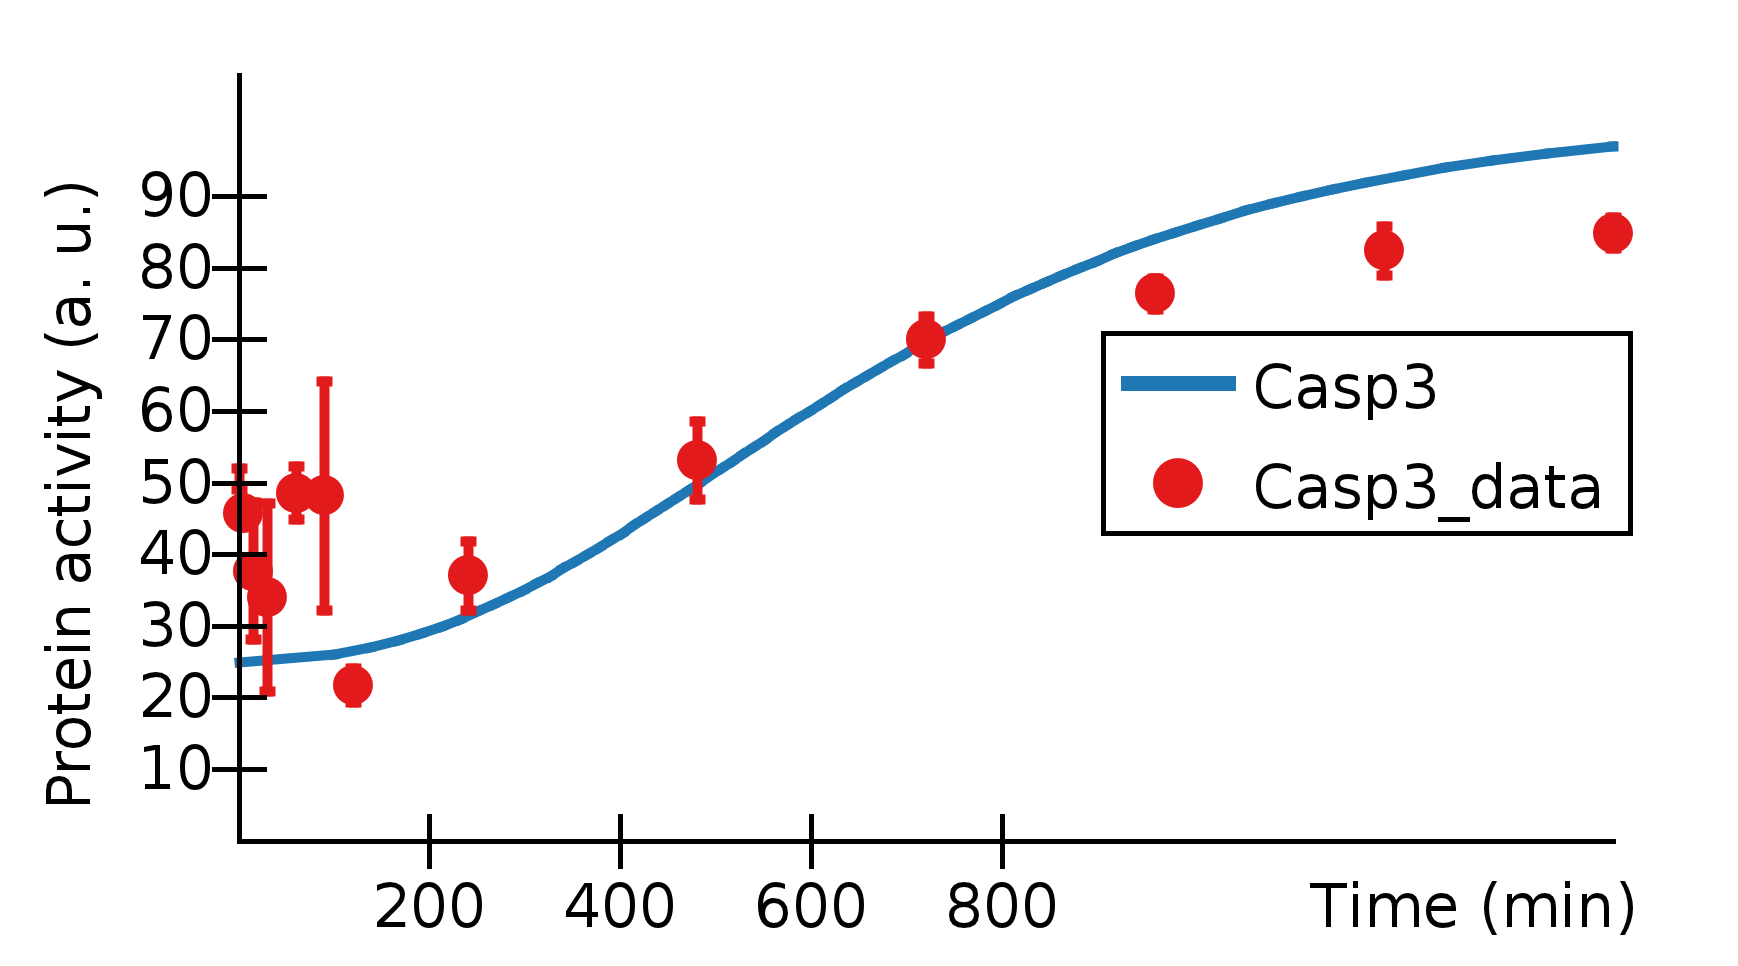
\includegraphics[width=0.29\textwidth]{images/TNFa100/casp3}} \\
\subfloat[MEK (2 hours)]{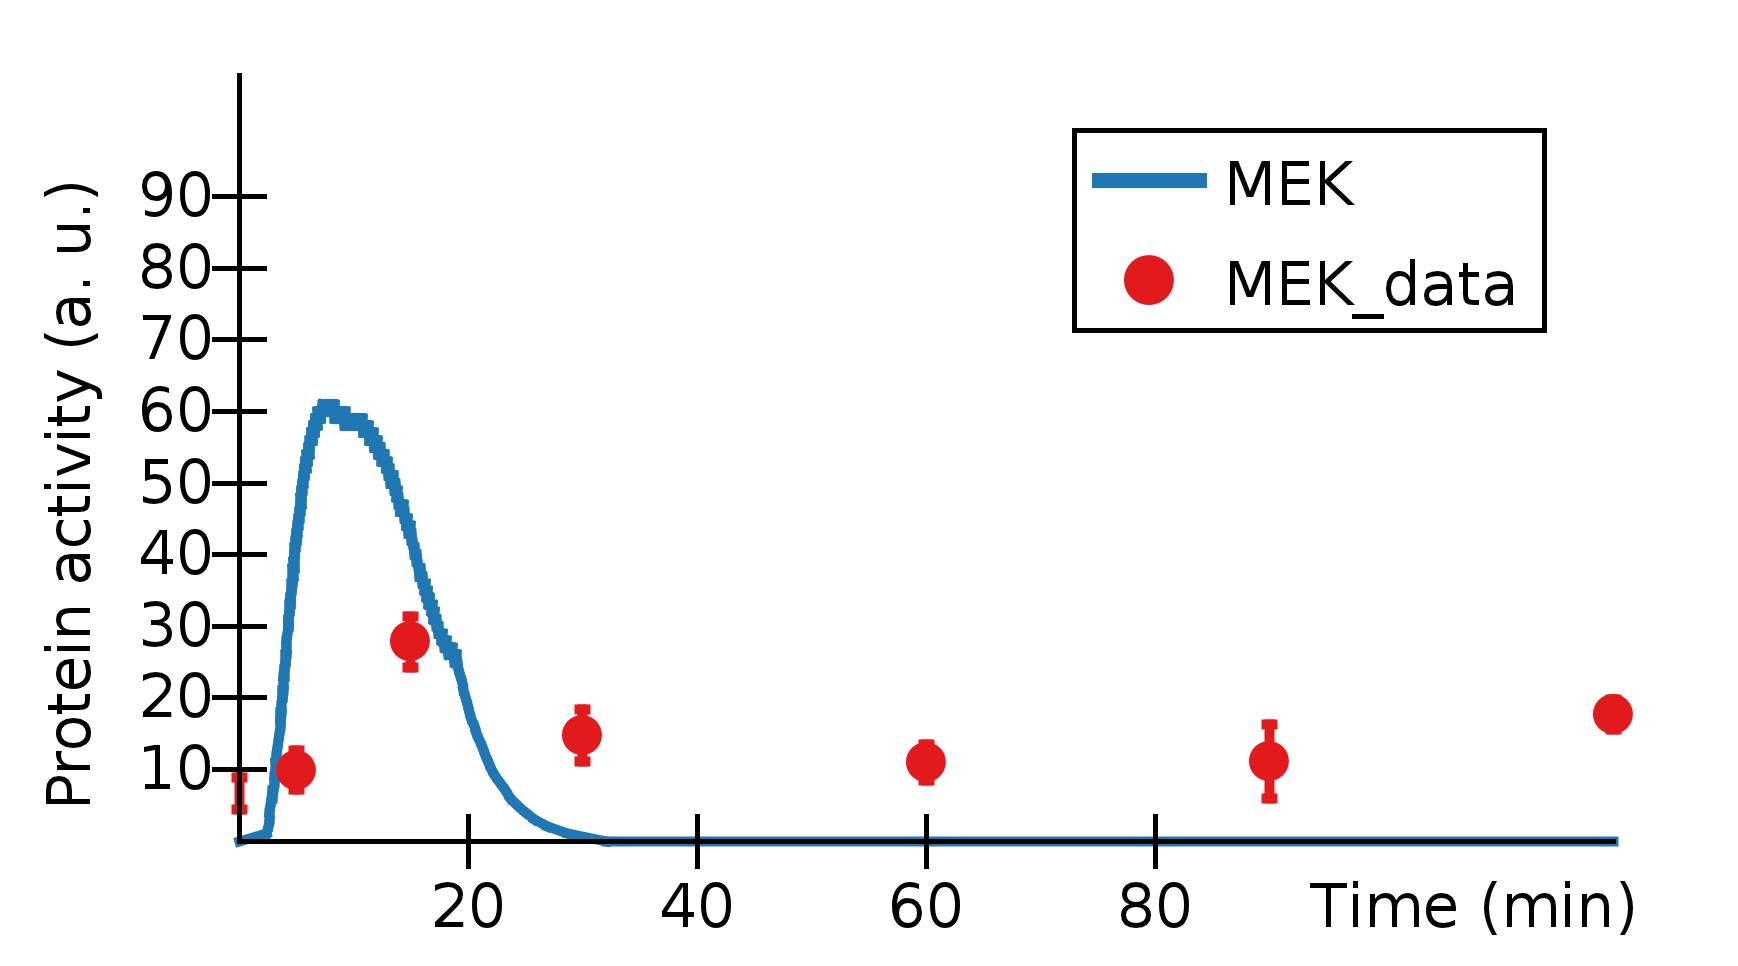
\includegraphics[width=0.29\textwidth]{images/TNFa100/MEK}} &
\subfloat[ERK (2 hours)]{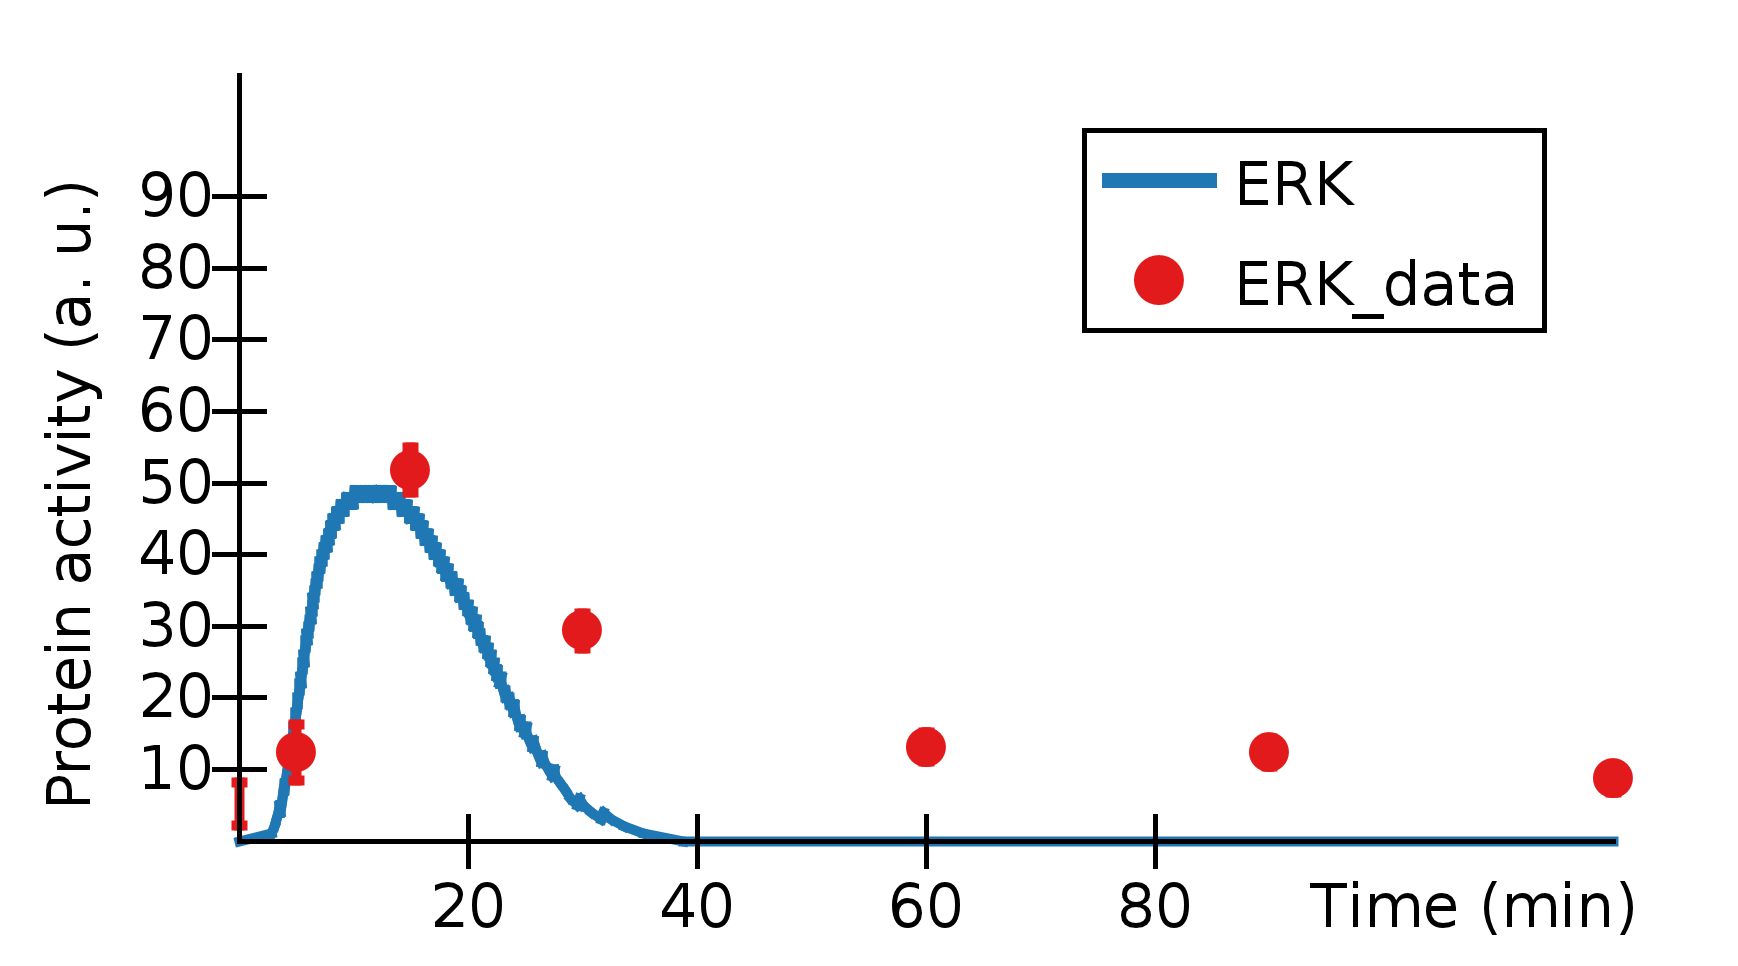
\includegraphics[width=0.29\textwidth]{images/TNFa100/ERK}} &
\subfloat[Akt]{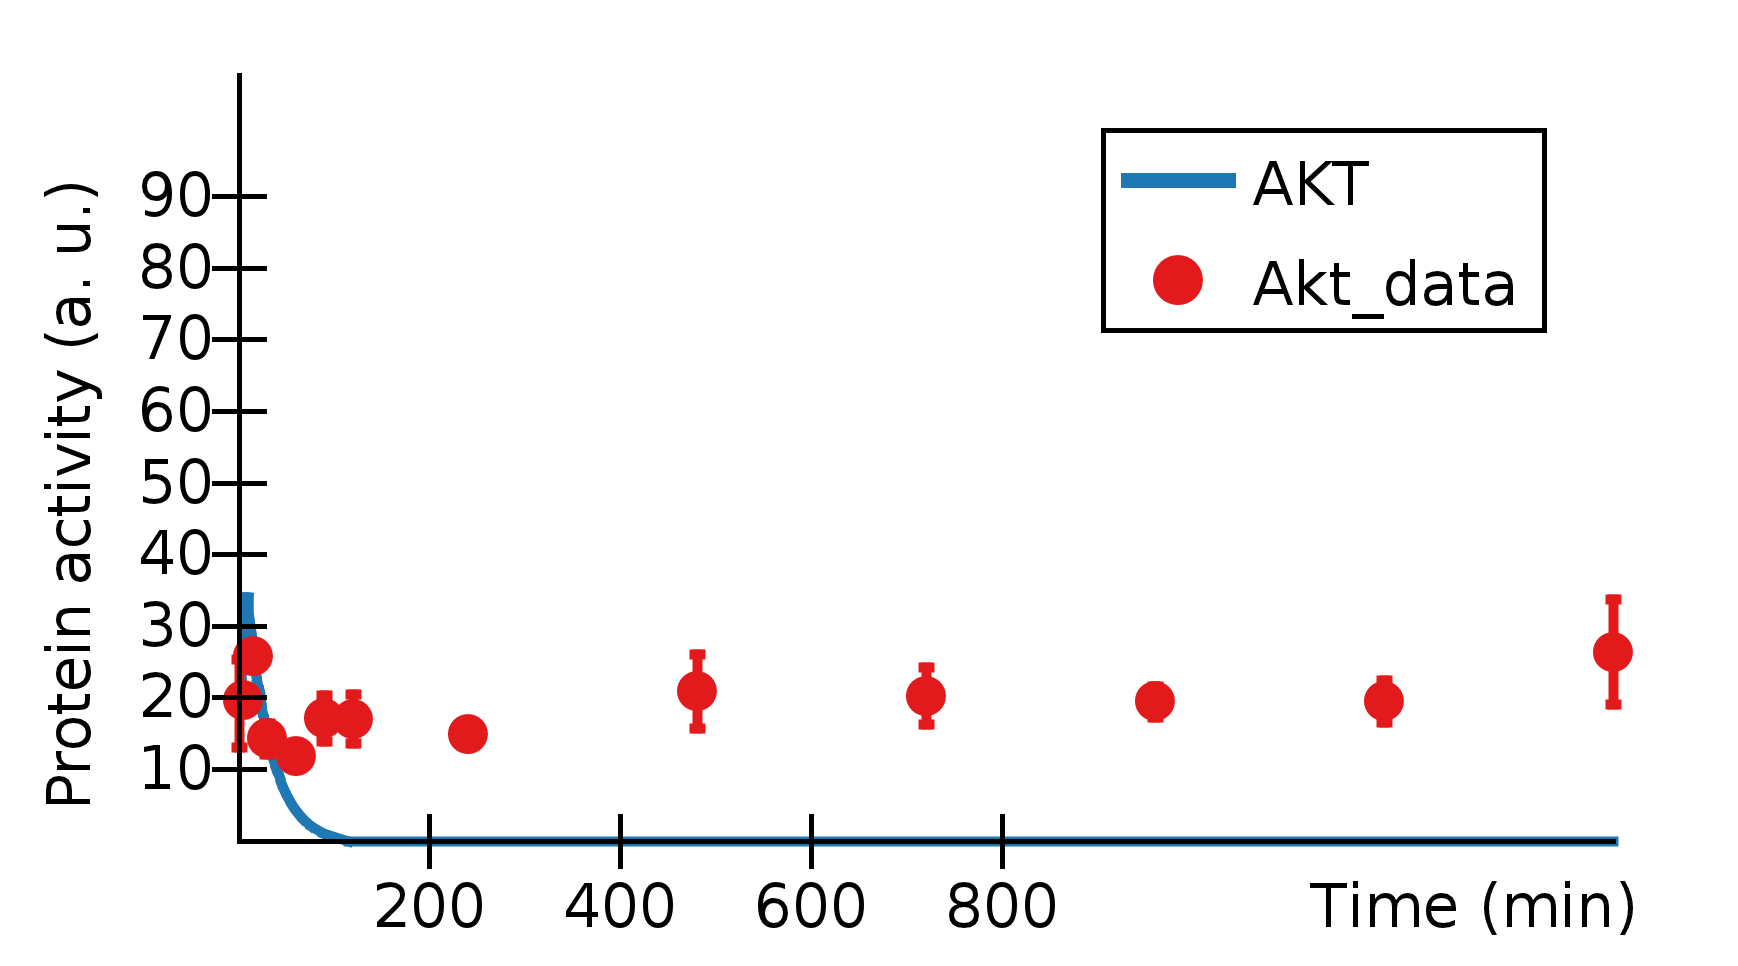
\includegraphics[width=0.29\textwidth]{images/TNFa100/Akt}} \\
\subfloat[IRS-1(S) (2 hours)]{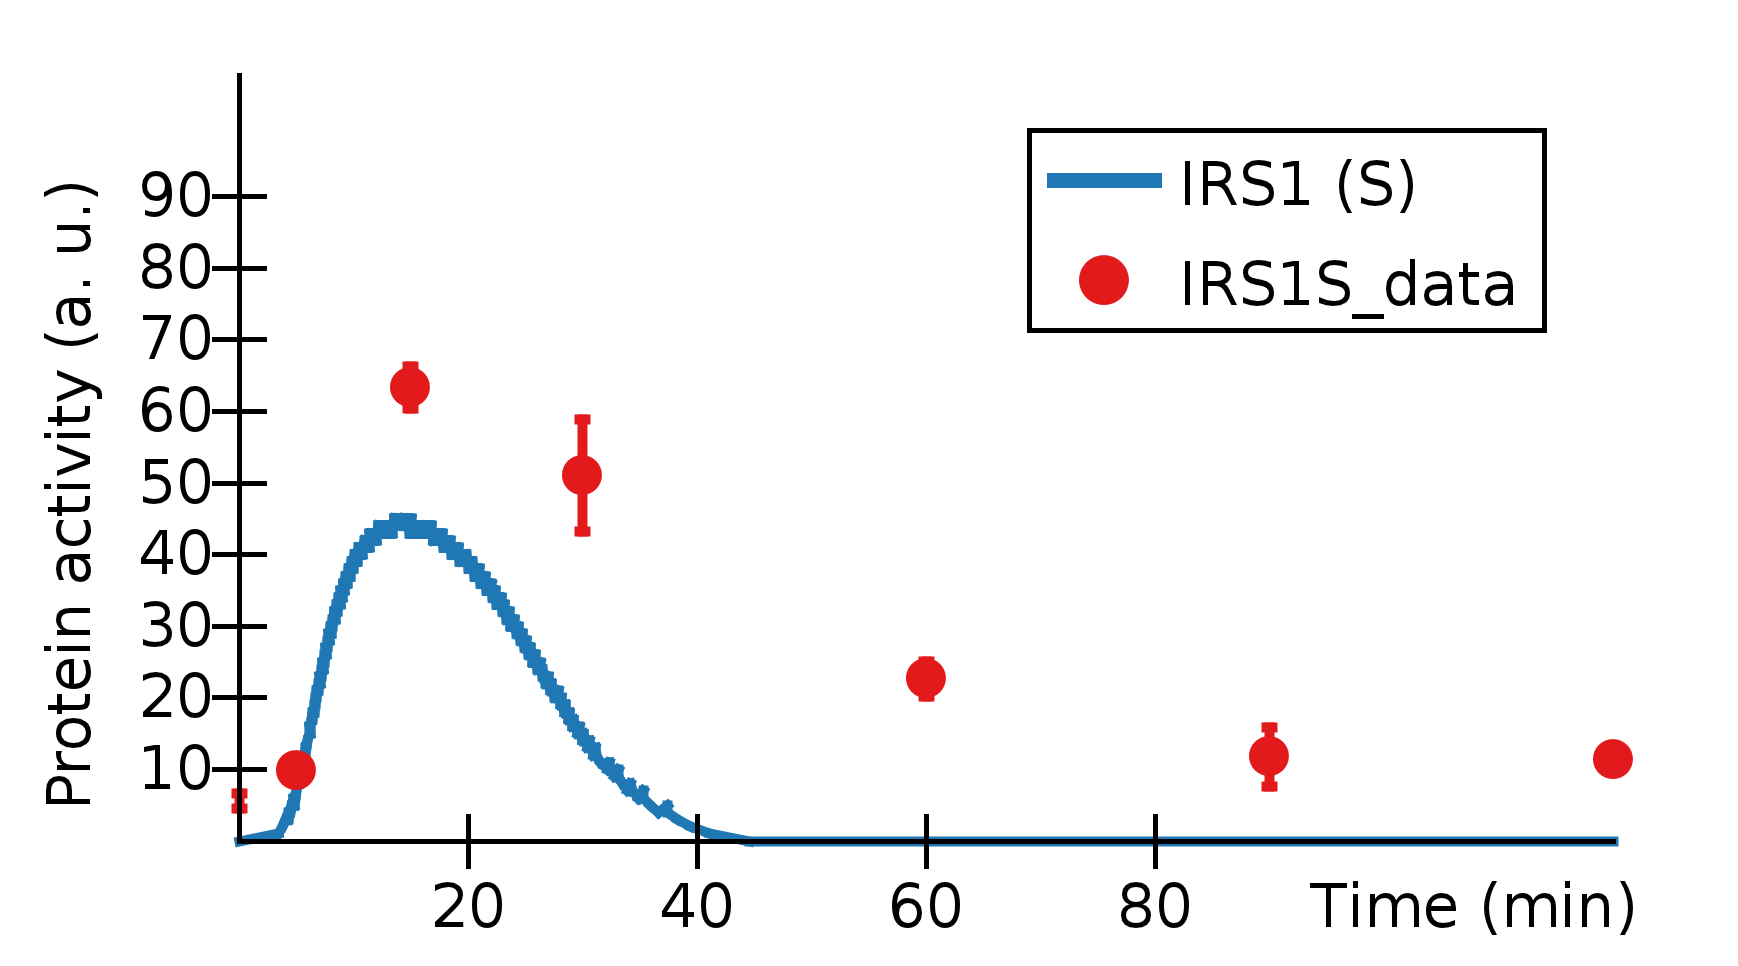
\includegraphics[width=0.29\textwidth]{images/TNFa100/IRS1s_120}} &
\subfloat[IRS-1(Y) (2 hours)]{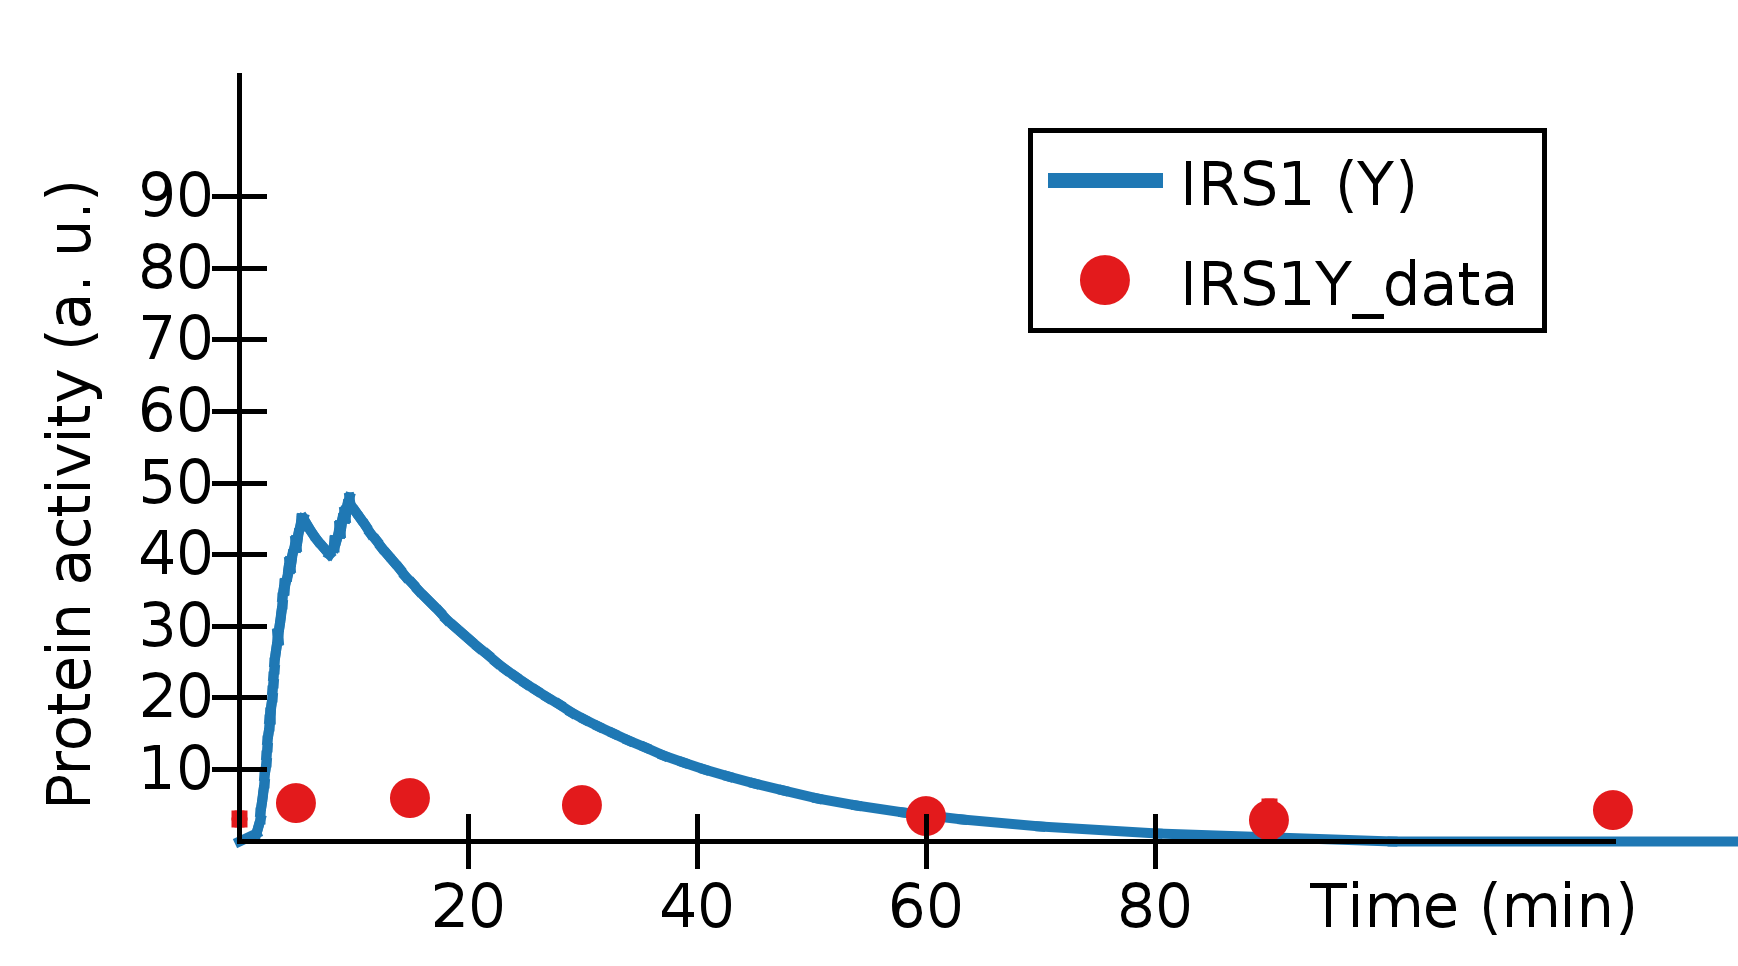
\includegraphics[width=0.29\textwidth]{images/TNFa100/IRS1y_120}} &
\subfloat[FKHR (12 hours)]{\includegraphics[width=0.29\textwidth]{images/TNFa100/FKHR_720}}
\end{tabularx}
\caption{Comparison between the ANIMO model in Figure~\ref{fig:large-model-complete} and experimental data. Treatment condition: 100 ng/ml TNF$\alpha$.
If not specified, the time span is 24 hours.}\label{fig:differences1}
\end{minipage}
\end{figure}


\begin{figure}[!tpb]
\begin{minipage}{\textwidth}
\begin{tabularx}{\textwidth}{XXX}
\subfloat[MK2 (2 hours)]{\includegraphics[width=0.29\textwidth]{images/EGF100/MK2}} &
\subfloat[JNK1 (2 hours)]{\includegraphics[width=0.29\textwidth]{images/EGF100/JNK1}} &
\subfloat[IKK]{\includegraphics[width=0.29\textwidth]{images/EGF100/IKK}} \\
\subfloat[caspase-8]{\includegraphics[width=0.29\textwidth]{images/EGF100/casp8}} &
\subfloat[caspase-3]{\includegraphics[width=0.29\textwidth]{images/EGF100/casp3}} &
\subfloat[MEK (2 hours)]{\includegraphics[width=0.29\textwidth]{images/EGF100/MEK}} \\
\subfloat[ERK (2 hours)]{\includegraphics[width=0.29\textwidth]{images/EGF100/ERK}} &
\subfloat[Akt (2 hours)]{\includegraphics[width=0.29\textwidth]{images/EGF100/Akt_120}} &
\subfloat[Akt]{\includegraphics[width=0.29\textwidth]{images/EGF100/Akt_1440}} \\
\subfloat[IRS-1(S) (2 hours)]{\includegraphics[width=0.29\textwidth]{images/EGF100/IRS1s_120}} &
\subfloat[IRS-1(Y) (2 hours)]{\includegraphics[width=0.29\textwidth]{images/EGF100/IRS1y_120}} &
\subfloat[IRS-1(Y) (12 hours)]{\includegraphics[width=0.29\textwidth]{images/EGF100/IRS1y_720}} \\
\subfloat[FKHR (2 hours)]{\includegraphics[width=0.29\textwidth]{images/EGF100/FKHR_120}} &
\subfloat[FKHR (12 hours)]{\includegraphics[width=0.29\textwidth]{images/EGF100/FKHR_720}}
\end{tabularx}
\caption{Comparison between the ANIMO model in Figure~\ref{fig:large-model-complete} and experimental data. Treatment condition: 100 ng/ml EGF.
If not specified, the time span is 24 hours.}\label{fig:differences2}
\end{minipage}
\end{figure}


\begin{figure}[!tpb]
\begin{minipage}{\textwidth}
\begin{tabularx}{\textwidth}{XXX}
\subfloat[MK2 (2 hours)]{\includegraphics[width=0.29\textwidth]{images/TNFa100_EGF100/MK2}} &
\subfloat[JNK1 (2 hours)]{\includegraphics[width=0.29\textwidth]{images/TNFa100_EGF100/JNK1}} &
\subfloat[IKK]{\includegraphics[width=0.29\textwidth]{images/TNFa100_EGF100/IKK}} \\
\subfloat[caspase-8]{\includegraphics[width=0.29\textwidth]{images/TNFa100_EGF100/casp8}} &
\subfloat[caspase-3]{\includegraphics[width=0.29\textwidth]{images/TNFa100_EGF100/casp3}} &
\subfloat[MEK (2 hours)]{\includegraphics[width=0.29\textwidth]{images/TNFa100_EGF100/MEK}} \\
\subfloat[ERK (2 hours)]{\includegraphics[width=0.29\textwidth]{images/TNFa100_EGF100/ERK}} &
\subfloat[Akt (2 hours)]{\includegraphics[width=0.29\textwidth]{images/TNFa100_EGF100/Akt}} &
\subfloat[IRS-1(S) (2 hours)]{\includegraphics[width=0.29\textwidth]{images/TNFa100_EGF100/IRS1s_120}} \\
\subfloat[IRS-1(S) (12 hours)]{\includegraphics[width=0.29\textwidth]{images/TNFa100_EGF100/IRS1s_720}} &
\subfloat[IRS-1(Y) (2 hours)]{\includegraphics[width=0.29\textwidth]{images/TNFa100_EGF100/IRS1y}} &
\subfloat[FKHR (4 hours)]{\includegraphics[width=0.29\textwidth]{images/TNFa100_EGF100/FKHR_240}}
\end{tabularx}
\caption{Comparison between the ANIMO model in Figure~\ref{fig:large-model-complete} and experimental data. Treatment condition: 100 ng/ml TNF$\alpha$ + 100 ng/ml EGF.
If not specified, the time span is 24 hours.}\label{fig:differences3}
\end{minipage}
\end{figure}


\end{document}
